\cleardoublepage

\chapter{Elektrostatiğe Giriş}

Elektrodinamiğin tartışılmasına, zamandan bağımsız yük ve alan dağılımlarını kapsayan olaylarla, yani elektrostatik konusu ile başlıyoruz. Bu kısım okuyucuların çoğu için bir tekrar niteliğindedir. Bu bölümde fazla bir şey yapmayıp, ilerdeki tartışmalarda gerekli olan kavram ve tanımları ortaya koyacak ve bazı temel matematiksel araçları vereceğiz. Daha sonraki bölümlerde matematiksel teknikleri geliştireceğiz ve uygulayacağız.

Fiziğin şu yanına değinilmelidir. Tarihsel açıdan elektrostatik büyük-boyuttaki (makroskobik) olayların bilimi olarak geliştirilmiştir. Giriş'in sonunda da belirtildiği gibi, noktasal yük ya da bir noktadaki elektriksel alan gibi soyutlamalar, büyük-boyuttaki olayların anlatılmasına yarayan matematiksel yapılar olarak görülmeli ve bunların küçük-boyuttaki (mikroskobik) düzeyde anlamlarını yitirebilecekleri unutulmamalıdır.


\section{Coulomb Kanunu}

Elektrostatiğin tümü, birbirlerine göre duran iki yüklü cisim arasındaki kuvvetin nicel ifadesini veren Coulomb yasasından çıkmaktadır. Coulomb, yaptığı deneyler sonucunda, hava içerisinde kendi boyutlarına göre birbirlerinden çok uzakta bulunan yüklü iki küçük cisim arasındaki kuvvetin,

\begin{enumerate}
  \item her bir yükün büyüklüğüyle doğru orantılı olduğunu,
  \item aradaki uzaklığın karesiyle ters orantılı olarak değiştiğini, 
  \item yükleri birleştiren çizgi boyunca yöneldiğini ve
  \item cisimler zıt olarak yüklüyseler çekici, aynı yükle yüklüyseler itici

\end{enumerate}

olduğunu göstermiştir. Ayrıca deneysel olarak gösterilmiştir ki, yüklü bir küçük cisim üzerine dolayında bulunan diğer yüklü küçük cisimlerin uyguladıkları toplam kuvvet, her çift arasındaki Coulomb kuvvetlerinin vektörel toplamına eşittir. Kesin olarak söylemek gerekirse, Coulomb'un sonuçları, boşluktaki ya da geçirgenliği (susceptibility) önemsenmeyen ortamlardaki yüklere uygulanır. Dielektriksel ortamlardaki yüklerin ele alınışını 4. bölüme bırakıyoruz.


\begin{theorem}
    
\[ \Vec{F} = k q_{1} q_{2} \dfrac{\Vec{x_{1} - \Vec{x_{2}}}}{|\Vec{x_{1}} - \Vec{x_{2}}|^{3}} \ (1.2)\]        
\[ k = \dfrac{1}{4 \pi \varepsilon_{0}}  \]
\[ k = 9 \times 10^{9} \dfrac{N m^{2}}{C^{2}},  \ \varepsilon_{0} = 8.85 \times 10^{-12} \dfrac{C^{2}}{N m^{2}} \]

Aslında şöyle yazıyorduk,
    \[ \Vec{F} = k  \dfrac{q_{1} q_{2} }{r^{2}} \hat{r} \dfrac{r}{r} \]   
    \[ = k \dfrac{q_{1} q_{2} \Vec{r} }{r^{3}} \]  
     
\begin{figure}[H]
    \centering
     \begin{tikzpicture}
        \coordinate (O) at (0.0,0.0);
        \coordinate (Q1) at (1.0,1.1);
        \coordinate (Q2) at (2.0,.1);
        \coordinate (F1) at ($(Q1)+(Q1)-(Q2)$);
        \coordinate (F2) at ($(Q2)+(Q2)-(Q1)$);
        
        \node[point, charge color] (Q1 node) at (Q1) 
            [label={east, yshift=1mm, charge color}:$q_1$ Gözlem noktası] {} 
            edge[arr] node[at end, above] {$\vec F_1$} (F1);
        \node[point, charge color] (Q2 node) at (Q2) 
            [label={east, yshift=1mm, charge color}:$q_2$ Kaynak noktası] {} 
            edge[arr] node[at end, below] {$\vec F_2$} (F2)
            edge[arr] node[midway, right, yshift=1mm, xshift=1mm] {$\vec x_1-\vec x_2$} (Q1 node);
        \node[point] at (O)
        [label={west}:O] {} 
        edge[arr] node[midway, below] {$\vec{x}_2$} (Q2 node)
        edge[arr] node[midway, anchor=south east] {$\vec{x}_1$} (Q1 node);
    \end{tikzpicture}
    \caption*{Coulomb Kanunu}
\end{figure}
\end{theorem}


\section{Elektrik Alanı}

Ölçülen nicelik kuvvet olmakla birlikte, kuvvetten bir basamak ötede bulunan bir kavramı, yüklü cisimler topluluğunun elektrik alanı kavramını tanımlamak yararlıdır. Şimdilik elektrik alanını, verilen bir noktada birim yük başına etkiyen kuvvet olarak tanımlayabiliriz. Yerin fonksiyonu olan bir vektördür ve $\Vec{E}$ ile gösterilir. Bununla birlikte, elektrik alanının tanımında dikkatli olunmalıdır. Bunun zorunlu olarak bir balmumu yuvarlağı üzerine yerleştirilen birim yükün söz konusu noktaya getirilmesiyle ölçülen kuvvet olması gerekmez. Nedeni açıktır. Bir birim yük öylesine büyük olabilir ki, orada bulunması yüklü cisimler topluluğunun alanını önemli ölçüde değiştirebilir. Bu nedenle bir limit süreci kullanılmalıdır, yani küçük bir sınama cismine etkiyen kuvvetin bu sınama cismi üzerindeki yüke oranı, iyice küçük yükler için ölçülmelidir* . Deneysel olarak, sınama yükü gitgide küçültüldükçe, bu oran ve kuvvetin yönü sabitleşmeye yüz tutacaktır. Büyüklüğün ve yönün bu limit değerleri, elektrik alanının söz konusu noktadaki büyüklüğünü ve yönünü tanımlar. Elektriksel alanın tanımını simgelerle şöyle yazabiliriz:
\begin{align}
    \Vec{F} = q \Vec{E}
\end{align}

Burada $\Vec{F}$ kuvveti, $\Vec{E}$ elektriksel alanı ve q yükü göstermektedir. Bu eşitlikte q yükünün bir noktaya sıkıştırıldığı, kuvvet ve alanın da bu noktada değerlendirildiği varsayılmaktadır.

Coulomb yasası da benzer şekilde yazılabilir. $\Vec{x_{1}}$ noktası sıkıştırılmış $q_{1}$ noktasal yükü üzerine  $\Vec{x_{2}}$ noktasına sıkıltırılmış başka bir $q_{2}$ noktasal yükü tarafından uygulanan kuvvet $\Vec{F}$ olmak üzere, Coulomb yasası
\begin{align}
    \Vec{F} = k q_{1} q_{2} \dfrac{\Vec{x_{1} - \Vec{x_{2}}}}{|\Vec{x_{1}} - \Vec{x_{2}}|^{3}}
\end{align}

şeklinde simgelenir. $q_{1}$ ve $q_{2}$'nin pozitif ve negatif değerler alabilen cebirsel nicelikler olduğuna dikkat ediniz. k orantı katsayısı ise kullanılan birim sistemine bağlıdır.

$\Vec{x_{1}}$ noktasındaki $q_{1}$ noktasal yükünün $\Vec{x}$ noktasında doğurduğu elektrik alanı, Şekil 1.1'de gösterildiği gibi doğrudan elde edilebilir:
\begin{align}
    \Vec{E} (\Vec{x}) = k q_{1} \dfrac{( \Vec{x} - \Vec{x_{1}})}{|\Vec{x} - \Vec{x_{1}}|^{3}}
\end{align}

k sabiti seçilen yük birimi tarafından belirlenir. Elektrostatik birimler (esb)'de birim yük, bir santimetre ötesine konan kendine eşit yüke 1 dyne'lik kuvvet uygulayan yük olarak seçilir. Buna göre CGS birimleriyle birlikte, $k = 1$'dir ve yük birimine "stat-coulomb" denir. MKS sisteminde $k = (4 \pi \varepsilon_{0})^{-1}$ olup, burada $\varepsilon_{0} $ ( $= 8.854 \times 10^{-12}$ farad/metre) boş uzayın elektriksel geçirgenliğidir. 
\begin{figure}[h!]
    \centering
    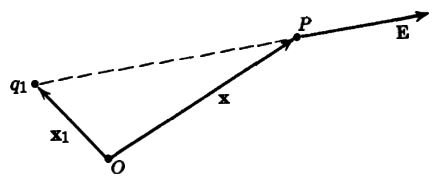
\includegraphics[width=6cm]{classical_electrodynamics/img/ch1/1.1.jpg}
    \caption{}
\end{figure}

\newpage

Çok sayıda yük tarafından oluşturulan kuvvetlerin deneysel olarak gözlenen çizgisel üst-üste gelme ilkesi, $\Vec{x}_{i}$ noktalarında bulunan $q_{i} (i=1,2,...,n)$ noktasal yükler sisteminin $\Vec{x}$ noktasında oluşturduğu elektrik alanının
\begin{align}
    \Vec{E} (\Vec{x}) = k \sum_{i = 1}^{n} q_{i} \dfrac{( \Vec{x} - \Vec{x}_{i})}{| \Vec{x} - \Vec{x_{i}}|^{3}}
\end{align}

şeklinde vektörel bir toplam olarak yazılabileceğini söylemektedir. Eğer yükler çok küçük ve $\rho (\Vec{x}')$ yük yoğunluğuyla anlatılabilecek kadar çok sayıda iseler [$\Vec{x}'$ noktasındaki $\Delta x' \Delta y' \Delta z'$ küçük hacmi içinde $\Delta q$ yükü varsa, $\Delta q = \rho(\Vec{x}') \Delta x' \Delta y' \Delta z'$ yazılabilir], bu durumda üstteki toplam yerine bir integral gelir:
\begin{align}
   \Vec{E} (\Vec{x}) = k \int \rho(\Vec{x}') \dfrac{( \Vec{x} - \Vec{x}')}{| \Vec{x} - \Vec{x}'|^{3}} d^{3} x' 
\end{align}

Burada $d^{3} x' = dx' dy' dz'$, $\Vec{x}'$ noktasında üç boyutlu bir hacim elemanıdır.


\begin{theorem}
  \[  \lambda = \dfrac{q}{l} \ c/m  \rightarrow \textrm{ Çizgisel Yük Yoğunluğu}\] 
  \[  \sigma = \dfrac{q}{A} \ c/m^{2}  \rightarrow \textrm{ Yüzeysel Yük Yoğunluğu}\]
  \[  \rho = \dfrac{q}{V} \ c/m^{3} \rightarrow \textrm{ Hacimsel Yük Yoğunluğu} \]
  \[ \Delta q = \rho (\Vec{x}') \Delta x' \Delta y' \Delta z' \]
  \[ Q = \int_{V}  \rho (\Vec{x}') d^{3} x'  \]
Uzayın bir noktasındaki $\Vec{E} (\Vec{x})$ elektrik alanı,
 \[ \Vec{E} (\Vec{x}) = \dfrac{\Vec{F}}{q} = k q_{1} \dfrac{( \Vec{x} - \Vec{x}_{1})}{| \Vec{x} - \Vec{x_{1}}|^{3}} \]
Benzer şekilde n adet yük varlığında,
  \[ \Vec{E} (\Vec{x}) = k q_{1} \dfrac{( \Vec{x} - \Vec{x}_{1})}{| \Vec{x} - \Vec{x_{1}}|^{3}} + k q_{2} \dfrac{( \Vec{x} - \Vec{x}_{2})}{| \Vec{x} - \Vec{x_{2}}|^{3}} + ... =  k \sum_{i = 1}^{n} q_{i} \dfrac{( \Vec{x} - \Vec{x}_{i})}{| \Vec{x} - \Vec{x_{i}}|^{3}} \]
  \[ \Vec{E} (\Vec{x}) = k \sum_{i = 1}^{n} q_{i} \dfrac{( \Vec{x} - \Vec{x}_{i})}{| \Vec{x} - \Vec{x_{i}}|^{3}}\]
Sürekli yük dağılımı varsa,
\[   \Vec{E} (\Vec{x}) = k \int dq \dfrac{( \Vec{x} - \Vec{x}')}{| \Vec{x} - \Vec{x}'|^{3}}  \]
\[ \Vec{E} (\Vec{x}) = k \int \rho(\Vec{x}') \dfrac{( \Vec{x} - \Vec{x}')}{| \Vec{x} - \Vec{x}'|^{3}} d^{3} x' \ \tag{1.5}  \]
\[ d^{3} x' = dx' dy' dz' \]
\end{theorem}

\begin{definition}[The Dirac $\delta$ Fonksiyonu] \footnote{Lighthill, M.J. (1959). \textit{Introduction to Fourier Analysis and Generalised Functions}. Cambridge University Press.}
\[ \int_{-\infty}^{+ \infty} \delta(x) f(x) dx = f (0) \]
Eğer $f(x)$ herhangi bir iyi fonksiyonsa\footnote{\textit{good function}},
\[ \Big| \int_{-\infty}^{+ \infty}  \sqrt{\dfrac{n}{\pi}} e^{-n x^{2}} f(x) dx - f(0) \Big| \]
\[ = \Big| \int_{-\infty}^{+ \infty}  \sqrt{\dfrac{n}{\pi}} e^{-n x^{2}} \big[ f(x) - f(0) \big] dx \Big|  \]
\[ \leq \max \Big| \dfrac{d f(x)}{dx} \Big| \int_{-\infty}^{+ \infty} \sqrt{\dfrac{n}{\pi}}  e^{-n x^{2}} |x| dx \]
\[ = \dfrac{1}{\sqrt{n \pi}} \max \Big| \dfrac{d f(x)}{dx} \Big|_{n \rightarrow \infty} \rightarrow 0 \]
\end{definition}

\begin{theorem}
$\Vec{r}_{k}$ noktalarında bulunan N tane $q_{k}$ nokta yükünden oluşan yük yoğunluğu tanımlayalım:
\[ \rho (\Vec{x}) = \sum_{k=1}^{N} q_{k} \delta (\Vec{x} - \Vec{x}_{k}) \tag{1.6} \]
Denklem (1.5)'de yerine koyalım,
\[ f(a) = \int f (x) \delta(x-a) dx \]
\[ \Vec{E} (\Vec{x}) = k \int \dfrac{\big\{ \sum_{k} q_{k} \delta(\Vec{x}' - \Vec{x}_{k}) \big\} ( \Vec{x} - \Vec{x}') }{| \Vec{x} - \Vec{x}'|^{3}} d^{3} x' \]
\[ = k \sum_{k} q_{k} \int \dfrac{ ( \Vec{x} - \Vec{x}')}{| \Vec{x} - \Vec{x}'|^{3}} \delta(x' - x_{k}) d^{3} x'\]
\[ \Vec{E} (\Vec{x}) = k \sum_{k} q_{k} \dfrac{\Vec{x} - \Vec{x}'}{| \Vec{x} - \Vec{x}'|^{3}} \]
Denklem (1.4) yeniden elde edildi.
\begin{note}
Dirac $\delta$'nın tanımına bak!
\end{note}
\end{theorem}

Bu noktada Dirac $\delta$ fonksiyonunu tanımlamak yararlıdır. Bir boyutta $\delta(x-a)$ şeklinde yazılan $\delta$ fonksiyonu, matematiksel açıdan dürüst bir fonksiyon olmayıp aşağıdaki özelliklere sahiptir:

\begin{enumerate}
  \item $x \neq a$ için $\delta(x-a) = 0$'dır.
  \item İntegrasyon bölgesi $x=a$'yı kapsıyorsa  $\int \delta(x-a) dx = 1$'dir, kapsamıyorsa bu integral sıfırdır. \\ 
 Delta fonksiyonuna, güçlü olmamakla birlikte, sezgisel bir anlam verilebilir. Çan eğrisi gibi doruklu bir eğrinin, altındaki alanı sabit tutmak koşuluyla, doruğu yükseltilirken genişliği gitgide azaltılırsa limit durumda delta fonksiyonuna varılır. Delta fonksiyonlarına ve kullanımlarına kapsamlı ve güçlü bir matematiksel yaklaşım, Schwartz'ın dağılımlar teorisidir. \\
 \ 
 
\quad Yukarıdaki tanımlardan açıkça görüleceği gibi, keyfi bir $f(x)$ fonksiyonu için 
  \item $\int f (x) \delta(x-a) dx = f(a)$'dır.

  Delta fonksiyonunun iyi-davranışlı fakat çok keskin doruklu bir fonksiyon olduğu düşünülürse, $f(x)$ fonksiyonu ile delta fonksiyonunun türevinin integrali kolayca kurulabilir. Buna göre tanım şu şekildedir:
  \item $\int f (x) \delta'(x-a) dx = - f'(a)$'dır.
  \\
  Burada üs işareti argümana göre türevlendirmeyi göstermektedir.
  
  \
  \quad Delta fonksiyonunun argümanı, bağımsız x değişkeninin bir $f(x)$ fonksiyonu ise, bu delta fonksiyonu şu kurala göre dönüştürülebilir:
  \item $\delta (f(x)) = \sum_{i} \dfrac{1}{\big| \frac{df}{dx} (x_{i}) \big|} \delta (x - x_{i})$ 
  \\
  $f(x)$'in sadece basit sıfırlara sahip olduğu ve bu sıfırların (yani $f(x) = 0$ denkleminin köklerinin) $x = x_{i}$ noktalarında bulunduğu varsayılmaktadır.

  Birden fazla boyutta, sadece her bir boyuttaki delta fonksiyonlarının çarpımlarını alırız. Örneğin üç boyutta, kartezyen koordinatlarla çalıştığımızda,

  \item $\delta(\Vec{x} - \Vec{X}) = \delta (x_{1} - X_{1}) \delta (x_{2} - X_{2}) \delta (x_{3} - X_{3})   $ \\
  $\Vec{x} = \Vec{X}$ noktasının dışında her yerde sıfır olan bir fonksiyondur ve şu koşulları sağlar:

  \item $\int_{\Delta V} \delta(\Vec{x} - \Vec{X}) d^{3}x =   \begin{cases}
      1, & \text{eğer $\Delta V$ hacmi $\Vec{x} = \Vec{X}$ noktasını kapsıyorsa}\\
      0, & \text{eğer $\Delta V$ hacmi $\Vec{x} = \Vec{X}$ noktasını kapsamıyorsa}
    \end{cases}   $ \\
    Uzayın boyutu ne ise, delta fonksiyonunun da buna uygun hacmin tersine eşit bir boyuta sahip olduğuna dikkat ediniz.

\end{enumerate}

    Noktasal yüklerin kesikli bir cümlesi, delta fonksiyonları kullanılarak bir yük yoğunluğu ile betimlenebilir. Örneğin,

    \begin{align}
        \rho ( \Vec{x}) = \sum_{i=1}^{n} q_{i} \delta (\Vec{x} - \Vec{x_{i}})
    \end{align}
$\Vec{x}_{i}$ noktalarına yerleşmiş n tane $q_{i}$ noktasal yükünün bir dağılımını göstermektedir. (1.6)'daki bu yük yoğunluğunu (1.5) ifadesinde yerine koyduktan sonra, delta fonksiyonunun özelliklerini kullanarak integralini alırsanız, (1.4)'deki kesikli toplamı elde edersiniz.

\section{Gauss Kanunu}

Denklem (1.5) integrali, elektrik alanını hesaplamak için her zaman en uygun form değildir. Gauss kanunu olarak adlandırılan ve bazı durumlarda çok daha yararlı olan ve ayrıca $\Vec{E} (\Vec{x})$ için bir diferansiyel denkleme yol açan başka bir integral sonucu vardır. Gauss kanununu elde etmek için, Şekil 1.2'de gösterildiği gibi, önce noktasal bir q yükü ve kapalı bir S yüzeyi alalım. q yükünden yüzey üzerindeki bir noktaya olan uzaklık r, bu noktada yüzeye dik olan dışa doğru yönelmiş birim vektör $\Vec{n}$ ve yüzey elemanı $da$ olsun. q yükünün yüzey üzerindeki noktada oluşturduğu $\Vec{E}$ elektrik alanı $\Vec{n}$ ile $\theta$ açısı yapıyorsa, bu durumda $\Vec{E}$'nin yüzeye dik bileşeni çarpı yüzey elemanı şu olur:

\begin{align}
    \Vec{E} \cdot \Vec{n} \ da = k q \dfrac{\cos \theta}{r^{2}} da
\end{align}

\begin{figure}[h!]
\centering
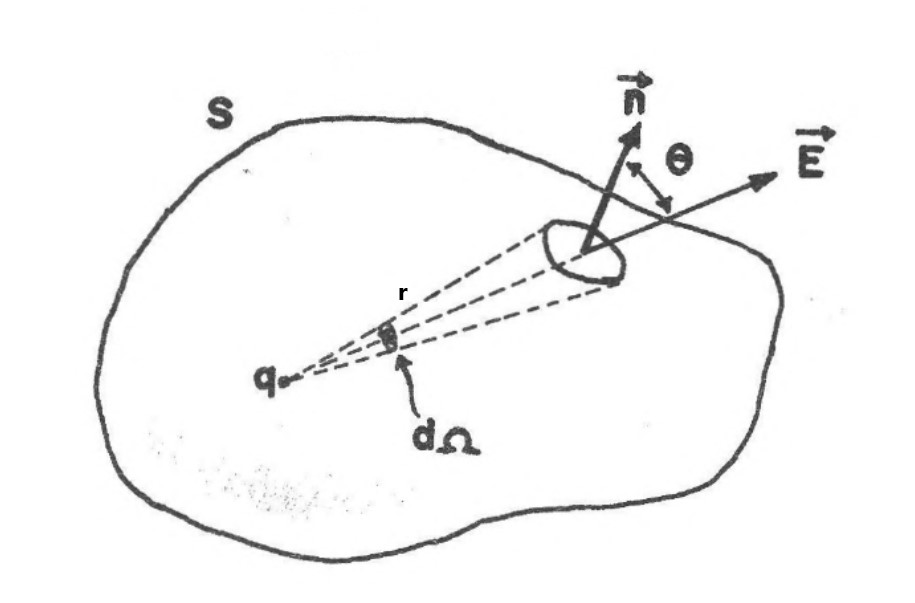
\includegraphics[width=8cm]{classical_electrodynamics/img/ch1/1.2.jpg}
\caption{}
\end{figure}  

\newpage

\begin{tcolorbox}
Gauss kanununun mantığı aslında akı kavramına dayanır. Zaten diferansiyel formunu elde edebilmek için diverjans formülünü kullanmamız gerekir. Diverjansın anlamı da akı demektir.
\end{tcolorbox}
\begin{theorem}
Elektrik alanı radyal yönde tanımlayalım,
\[ \Vec{E} = k \dfrac{q}{r^{2}} \hat{r}  \]
Her iki tarafı $\hat{n}$ ile skaler olarak çarpalım,
\[ \Vec{E} \cdot \hat{n} = k  \dfrac{q }{r^{2}} \hat{r} \cdot \hat{n} = k \dfrac{q}{r^{2}} \cos \theta \]
Her iki tarafın kapalı bir yüzey üzerinden integralini alalım,
\[ \oint_{S} \Vec{E} \cdot \hat{n} da = kq \int \dfrac{\cos \theta}{r^{2}} da \]


\begin{figure}[H]
\centering

\tikzset{every picture/.style={line width=0.75pt}} %set default line width to 0.75pt        

\begin{tikzpicture}[x=0.75pt,y=0.75pt,yscale=-1,xscale=1]
\centering
%uncomment if require: \path (0,396); %set diagram left start at 0, and has height of 396

%Shape: Circle [id:dp6164862496730389] 
\draw   (205.08,169.28) .. controls (222.27,144.3) and (256.46,137.98) .. (281.44,155.17) .. controls (306.42,172.36) and (312.74,206.55) .. (295.55,231.53) .. controls (278.36,256.51) and (244.17,262.83) .. (219.19,245.64) .. controls (194.21,228.45) and (187.89,194.26) .. (205.08,169.28) -- cycle ;
%Straight Lines [id:da6091724811609507] 
\draw    (250.31,200.41) -- (306.42,199.75) ;
%Straight Lines [id:da37867790339611473] 
\draw    (250.31,200.41) -- (298.42,170.75) ;
%Shape: Free Drawing [id:dp5416442125918929] 
\draw  [line width=0.75] [line join = round][line cap = round] (262.42,193.46) .. controls (263.98,193.46) and (264.35,198.82) .. (264.42,199.46) ;
%Shape: Circle [id:dp6583870476509581] 
\draw   (405.08,169.28) .. controls (422.27,144.3) and (456.46,137.98) .. (481.44,155.17) .. controls (506.42,172.36) and (512.74,206.55) .. (495.55,231.53) .. controls (478.36,256.51) and (444.17,262.83) .. (419.19,245.64) .. controls (394.21,228.45) and (387.89,194.26) .. (405.08,169.28) -- cycle ;
%Shape: Ellipse [id:dp8683450578259656] 
\draw  [dash pattern={on 0.84pt off 2.51pt}] (397.42,200.25) .. controls (397.42,193.9) and (421.37,188.75) .. (450.92,188.75) .. controls (480.46,188.75) and (504.42,193.9) .. (504.42,200.25) .. controls (504.42,206.6) and (480.46,211.75) .. (450.92,211.75) .. controls (421.37,211.75) and (397.42,206.6) .. (397.42,200.25) -- cycle ;
%Straight Lines [id:da8972860917565987] 
\draw    (450.31,200.41) -- (504.42,200.25) ;
%Straight Lines [id:da8397046004404106] 
\draw    (450.31,200.41) -- (497.42,171.75) ;
%Shape: Ellipse [id:dp32056479533651416] 
\draw   (497.52,186.44) .. controls (494.8,179.35) and (494.1,173.02) .. (495.96,172.31) .. controls (497.82,171.6) and (501.53,176.76) .. (504.25,183.85) .. controls (506.98,190.94) and (507.67,197.27) .. (505.81,197.98) .. controls (503.95,198.7) and (500.24,193.53) .. (497.52,186.44) -- cycle ;
%Shape: Free Drawing [id:dp9391560143669213] 
\draw  [line width=0.75] [line join = round][line cap = round] (462.92,193.46) .. controls (464.48,193.46) and (464.85,198.82) .. (464.92,199.46) ;

% Text Node
\draw (278,201) node [anchor=north west][inner sep=0.75pt]  [font=\scriptsize]  {$r$};
% Text Node
\draw (269,188.9) node [anchor=north west][inner sep=0.75pt]  [font=\scriptsize]  {$\theta $};
% Text Node
\draw (311,174.9) node [anchor=north west][inner sep=0.75pt]    {$S$};
% Text Node
\draw (219,272.9) node [anchor=north west][inner sep=0.75pt] {\quad $S= r\theta$};
% Text Node
\draw (473,173.4) node [anchor=north west][inner sep=0.75pt]  [font=\scriptsize]  {$r$};
% Text Node
\draw (467.96,192.98) node [anchor=north west][inner sep=0.75pt]  [font=\tiny]  {$\si{\Omega}$};
% Text Node
\draw (511,177.9) node [anchor=north west][inner sep=0.75pt]    {$A$};
% Text Node
\draw (418.96,262.23) node [anchor=north west][inner sep=0.75pt]    {\quad $\si{\Omega}=\dfrac{A}{r^{2}}$};


\end{tikzpicture}
\end{figure}

\[ \oint_{S} \Vec{E} \cdot \hat{n} da = kq \oint \dfrac{\cos \theta}{r^{2}} da = kq \oint \dfrac{r^{2}d\Omega}{r^{2}} \]
\begin{align}
 d \Omega = \dfrac{\cos \theta da }{r^{2}}   
\end{align}
\[ \oint_{S} \Vec{E} \cdot \hat{n} da = kq  \begingroup \color{blue}{\underbrace{\oint_{S} d \Omega} _\text{$4\pi$} } \endgroup= kq 4\pi = \dfrac{1}{4 \pi \varepsilon_{0}} 4 \pi q = \dfrac{q}{\varepsilon_{0}}\]

q yükü S yüzeyinin dışında ise
\[ \oint \Vec{E} \cdot \hat{n} da =0\]
\[ d \Vec{a} = \hat{n} da\]
\[ \oint_{S} \Vec{E} \cdot \hat{n} da = \dfrac{1}{\varepsilon_{0}} \sum_{i} q_{i}  \tag{1.10} \]
\[ \oint_{S} \Vec{E} \cdot \hat{n} da = \dfrac{1}{\varepsilon_{0}} \int_{V} \rho(\Vec{x}) d^{3} x \tag{1.11} \]
Denklem (1.11), elektrostatiğin temel denklemlerinden biridir.

\begin{note}
 Diverjansın anlamı akı demektir.   
\end{note}
\end{theorem}

\section{Gauss Kanununun Diferansiyel Formu}

Gauss kanunu, elektrostatiğin temel integral formülasyonu olarak düşünülebilir. Diverjans teoremini kullanarak bir diferansiyel form (yani bir diferansiyel denklem) elde edebiliriz.

\begin{theorem}
\[ \grad = \dfrac{\partial}{\partial x} \hat{a}_{x} + \dfrac{\partial}{\partial y} \hat{a}_{y} + \dfrac{\partial}{\partial z} \hat{a}_{z}  \]  
\[ \grad \cdot \Vec{A} = \dfrac{\partial Ax}{\partial x}  + \dfrac{\partial Ay}{\partial y}  + \dfrac{\partial Az}{\partial z} \]  
\[ \oint_{S} \hat{A} \cdot \hat{n} da = \int_{V} ( \grad \cdot \Vec{A} ) d^{3} x\]
\[ \oint \Vec{E} \cdot \hat{n} da = \dfrac{q}{\varepsilon_{0}} = \dfrac{1}{\varepsilon_{0}} \int_{V} \rho d^{3}x \Rightarrow \int (\grad \cdot \Vec{E}) d^{3}x = \dfrac{1}{\varepsilon_{0}} \int \rho  d^{3} x  \]
\[ \grad \cdot \Vec{E} = \dfrac{\rho}{\varepsilon_{0}} \tag{1.13} \]
\end{theorem}

\section{Elektrostatiğin Diğer Bir Denklemi ve Skaler Potansiyeli}

(1.13) denklemi tek başına $\Vec{E}(\Vec{x})$ elektrik alanının üç bileşenini de tam olarak belirtmek için yeterli değildir. Belki de bazı okuyucular bilirler; uzayın her yerinde ıraksaması ve rotasyoneli verilirse, ancak o zaman bir vektör alanı hemen hemen tam olarak belirtilebilir. Bu nedenle $\Vec{E}(\Vec{x})$ rotasyonelini konumun fonksiyonu olarak veren bir denklem arıyoruz. Böyle bir denklem, yani
\begin{align*}
    \grad \times \Vec{E} = 0 \tag{1.14}
\end{align*}
denklemi doğrudan doğruya (1.5)'deki genelleştirilmiş Coulomb yasasından çıkar.
\begin{theorem}
\[   \grad \times \Vec{E} = 0 \]
\[ \Vec{E} = k \int \rho (\Vec{x}') \dfrac{(\Vec{x} - \Vec{x}') d^{3}x'}{|\Vec{x} - \Vec{x}'|^{3}}  \]
\[ \dfrac{\Vec{x - \Vec{x}'}}{|\Vec{x} - \Vec{x}'|^{3}} = - \grad \Big\{  \dfrac{1}{|\Vec{x} - \Vec{x}'|}  \Big\} \]
\[ |\Vec{x} - \Vec{x}'| = \sqrt{(x-x')^{2} + (y-y')^{2}  + (z-z')^{2} } \]
\[ \dfrac{\partial}{\partial x} \Big\{ \dfrac{1}{|\Vec{x}-\Vec{x}'|} \Big\} = \dfrac{\partial}{\partial x} \Big\{ \dfrac{1}{ \sqrt{(x-x')^{2} + (y-y')^{2}  + (z-z')^{2} }} \Big\} = \dfrac{\Vec{x - \Vec{x}'}}{|\Vec{x} - \Vec{x}'|^{3}} \]
Türevin ara işlemini yap! (İstersen $r$ diyebilirsin.)
\[ \Vec{E} (\Vec{x}) = -k \int \rho (\Vec{x}') \grad  \Big\{ \dfrac{1}{|\Vec{x}-\Vec{x}'|} \Big\} d^{3} x' \]
\[ = -\grad \underbrace{ k \int \rho (\Vec{x}') \dfrac{1}{|\Vec{x}-\Vec{x}'|} d^{3} x'}_{\phi (\Vec{x})} = - \grad \phi (\vec{x})\]
\[ \Vec{E} = -\grad \phi \]
Her 2 tarafı soldan $\grad$ ile çarpalım,
\[ \grad \times \Vec{E} = - \grad \times (\grad \phi) = 0 \] 
\end{theorem}
\begin{note}
\[ \dfrac{d}{dr} (\dfrac{1}{r}) = - \dfrac{1}{r^{2}}\]
\end{note}  

\newpage 

\begin{figure}[h!]
\centering
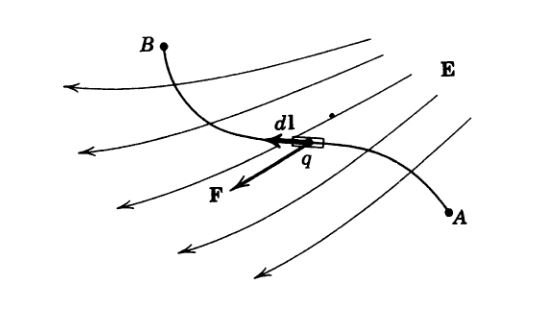
\includegraphics[width=7cm]{classical_electrodynamics/img/ch1/1.3.JPG}
\caption{}
\end{figure} 

\begin{theorem}
Skaler potansiyel elektrik alan içerisinde q deneme yükünü herhangi bir A noktasından B noktasına taşımak için yapılan iş düşünüldüğünde fiziksel bir anlama sahiptir.
\[\Vec{F} = q \Vec{E} \]
\[ W = - \int_{A}^{B} \Vec{F} \cdot d\Vec{l} = -q \int_{A}^{B} \Vec{E} \cdot d\Vec{l} \tag{1.18}\]
Alanın etkisine karşı yük üzerine yapılan işi hesapladığımız için eksi işaretini kullandık.
\[ \Vec{E} = - \grad \phi \Rightarrow W = q \int \grad \phi \cdot  d\Vec{l} \]
\[ \grad \phi \cdot  d\Vec{l} = \dfrac{\partial \phi}{\partial x} \hat{a}_{x} \cdot d_{x} = d \phi \]
\[ W = q \int_{A}^{B} \grad \phi \cdot  d\Vec{l} = q \int_{A}^{B} d \phi = q \big\{ \Phi(B) - \Phi(A) \big\} \tag{1.19} \]
Buna göre $q\phi$, elektrostatik alan içinde $q$ deneme yükünün potansiyel enerjisi olarak yorumlanabilir. Denklem (1.18) ve (1.19)'dan görülebileceği gibi, elektrik alanının iki nokta arasındaki çizgi integrali yoldan bağımsız olup, bu iki nokta arasındaki potansiyel farkının eksilisine eşittir.
\[ \int_{A}^{B} \Vec{E} \cdot d\Vec{l} = 0 \tag{1.20}\]
İntegral kapalı bir yol boyunca alınırsa,
\[ \oint \Vec{E} \cdot d\Vec{l} = 0 \tag{1.21} \]
Bunu da doğrudan doğruya Coulomb yasasından elde etmek olasıdır. Bu sonuca \textbf{Stokes teoremi}'nin uygulanması, bizi derhal $\grad \times \Vec{E} = 0$ denklemine geri götürür. Stokes teoremi: $\Vec{A}(\Vec{x})$ iyi davranışlı bir vektör alanı, S keyfi bir açık yüzey ve C'de S'yi sınırlayan kapalı bir eğri olmak üzere,
\[ \oint_{C} \Vec{A} \cdot d\Vec{l} = \int_{S} (\grad \times \Vec{A}) \cdot d\Vec{s} \]
burada $d\Vec{l}$, C'nin çizgi elemanıdır.
\[ \oint \Vec{E} \cdot d\Vec{l} = 0 \Rightarrow \int_{S} (\grad \times \Vec{E} ) \cdot d\Vec{s} = 0  \]
\[ \grad \times \Vec{E} = 0 \]
\[ \Phi (B) = \Phi (A) \]
\end{theorem}


\begin{tcolorbox}
$\dfrac{\Vec{x - \Vec{x}'}}{|\Vec{x} - \Vec{x}'|^{3}} = - \grad \Big\{  \dfrac{1}{|\Vec{x} - \Vec{x}'|}  \Big\}$ olduğunu gösterin.
\noindent Kartezyen koordinatlarda $\grad$ operatörü,
\begin{align*}
    \grad = \hat{x} \dfrac{\partial}{\partial x} + \hat{y} \dfrac{\partial}{\partial y} + \hat{z} \dfrac{\partial}{\partial z}
\end{align*}
Laplasyen,
\begin{align*}
  \grad \cdot \grad  =  \nabla^{2} = (  \hat{x} \dfrac{\partial}{\partial x} + \hat{y} \dfrac{\partial}{\partial y} + \hat{z} \dfrac{\partial}{\partial z} ) \cdot (  \hat{x} \dfrac{\partial}{\partial x} + \hat{y} \dfrac{\partial}{\partial y} + \hat{z} \dfrac{\partial}{\partial z} )
\end{align*}
\begin{align*}
    \nabla^{2} =  \dfrac{\partial^{2}}{\partial x^{2}} + \dfrac{\partial^{2}}{\partial y^{2}} + \dfrac{\partial^{2}}{\partial z^{2}} 
\end{align*}
Burada $|\Vec{x} - \Vec{x_{1}}| = r $ olarak alalım,
\begin{align*}
    \Vec{r} = x \hat{x} + y \hat{y} + z \hat{z}
\end{align*}
\begin{align*}
|r| = \sqrt{x^{2} + y^{2}  + z^{2} }
\end{align*}
\begin{align*}
  \grad(\dfrac{1}{r}) = \grad \big( \dfrac{1}{\sqrt{x^{2} + y^{2} + z^{2}}}  \big) 
\end{align*}
\begin{align*}
 \grad \big( \dfrac{1}{\sqrt{x^{2} + y^{2} + z^{2}}}  \big) = \big(  \hat{x} \dfrac{\partial}{\partial x} + \hat{y} \dfrac{\partial}{\partial y} + \hat{z} \dfrac{\partial}{\partial z} \big) \big( \dfrac{1}{\sqrt{x^{2} + y^{2} + z^{2}}}  \big)
\end{align*}
\begin{align*}
&= \hat{x}  \bigg\{ - \dfrac{1}{2} (x^{2} + y^{2} + z^{2})^{-3/2} (2x) \bigg\} \\
&\ + \hat{y} \bigg\{ - \dfrac{1}{2} (x^{2} + y^{2} + z^{2})^{-3/2} (2y) \bigg\} \\
&\ + \hat{z} \bigg\{ - \dfrac{1}{2} (x^{2} + y^{2} + z^{2})^{-3/2} (2z) \bigg\} 
\end{align*}
\begin{align*}
    = - \dfrac{(x^{2} + y^{2} + z^{2})^{-3/2}}{2}  \bigg\{ 2x \hat{x} + 2y \hat{y} + 2z \hat{z} \bigg\} 
\end{align*}
\begin{align*}
    = - \dfrac{(x^{2} + y^{2} + z^{2})^{-3/2}}{\cancel{2}} \cancel{2} \bigg\{ x \hat{x} + y \hat{y} + z \hat{z} \bigg\} 
\end{align*}
\begin{align*}
    = - \dfrac{1}{(x^{2} + y^{2} + z^{2})^{3/2}} \bigg\{ x \hat{x} + y \hat{y} + z \hat{z} \bigg\} 
\end{align*}
\begin{align*}
\grad (\dfrac{1}{r})= -\dfrac{\Vec{r}}{r^{3}}
\end{align*}
\begin{align*}
|\Vec{x} - \Vec{x_{1}}| = r \rightarrow \grad \dfrac{1}{|\Vec{x} - \Vec{x}_{1}|}= - \dfrac{(\Vec{x} - \Vec{x_{1}})}{|\Vec{x} - \Vec{x_{1}}|^{3}}
\end{align*}
\begin{align*}
 \nabla^{2} \Big( \dfrac{1}{|\Vec{x} - \Vec{x_{1}}|} \Big) = - \grad \cdot \bigg( \dfrac{(\Vec{x} - \Vec{x_{1}})}{|\Vec{x} - \Vec{x_{1}}|^{3}} \bigg)
\end{align*}
\end{tcolorbox}

\newpage

\begin{definition}[Poisson ve Laplace Denklemleri]
\[ \grad \cdot \Vec{E} = \dfrac{\rho}{\varepsilon_{0}} \Rightarrow \Vec{E} = - \grad \phi \] 
\[ \grad \cdot (- \grad \phi ) = -\nabla^{2} \phi = \dfrac{\rho}{\varepsilon_{0}} \Rightarrow \nabla^{2} \phi = - \dfrac{\rho}{\varepsilon_{0}} \]
Bu eşitliğe \textbf{Poisson} denklemi denir. Yük yoğunluğu olmayan uzay bölgelerinde, skaler potansiyel Laplace denklemini sağlar:
\[ \nabla^{2} \phi = 0 \tag{1.29} \]
Skaler potansiyelin bir çözümüne zaten daha önceden sahibiz:
\[ \phi (\Vec{x}) = k \int \dfrac{\rho (\Vec{x}')}{|\Vec{x} - \Vec{x}'|} d^{3}x' \]
Bu denklemi Poisson denkleminde yerine koyalım,
\[ \nabla^{2} \phi = \nabla^{2} \bigg\{ k \int \dfrac{\rho (\Vec{x}') d^{3} x' }{|\Vec{x} - \Vec{x'}|} \bigg\} \]
\[ = k \int \rho(\Vec{x}') \nabla^{2} \bigg\{ \dfrac{1}{|\Vec{x} - \Vec{x}'|} \bigg\} d^{3}x' \]
\[ \nabla^{2} \bigg\{ \dfrac{1}{|\Vec{x} - \Vec{x}'|}   \bigg\} = - 4 \pi \delta (\Vec{x} - \Vec{x}') \]
\[ \nabla^{2} \phi = k \int  \rho (\Vec{x}')  \bigg\{ -4 \pi \delta (\Vec{x} - \Vec{x}') \bigg\} d^{3}x' \]
\[ = - 4 \pi k \underbrace{\int \rho (\Vec{x}') \delta (\Vec{x} - \Vec{x}' ) d^{3}x'}_{\rho (\Vec{x})} = - \cancel{4 \pi} \dfrac{1}{\cancel{4 \pi}  \varepsilon_{0}} \rho(\Vec{x})  \]
\[ \nabla^{2} \phi = - \dfrac{\rho}{\varepsilon_{0}}  \tag{1.28}\]
Laplace Denkleminin yük yoğunluğunun olmadığı durumu:
\[ \nabla^{2} \phi = 0 \tag{1.29}\]
\end{definition}



\section{Yüklerin ve Dipollerin Yüzey Dağılımları, Potansiyel ve Elektrik Alandaki Süreksizlikler}
\subsection{Elektrostatiğin Sınır Koşulları}

Elektrostatiğin en genel problemerinden biri verilen yüzeysel dağılımın sebep olduğu potansiyelin veya elektrik alanın belirlenmesidir.

\begin{figure}[h!]
\centering
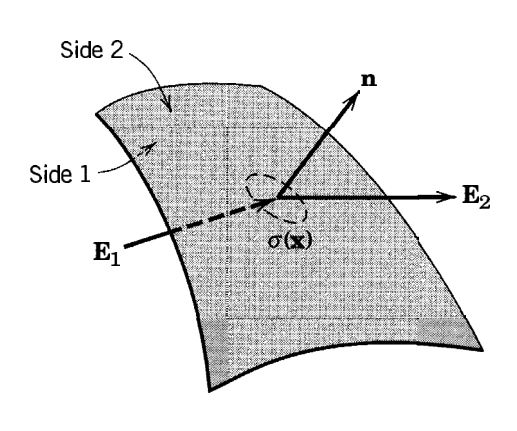
\includegraphics[width=5cm]{classical_electrodynamics/img/ch1/1.4.JPG}
\caption{Bir yük yüzeyini geçerken elektrik alanının dik bileşenindeki süreksizlik.}
\end{figure} 

\newpage
\begin{theorem}
\[ \sigma = \dfrac{dq}{da} \Rightarrow Q = \int_{S} \sigma da \]
\[ \sigma \rightarrow \dfrac{C}{m^{2}} \]
\begin{figure}[H]
\centering
\tikzset{
pattern size/.store in=\mcSize, 
pattern size = 5pt,
pattern thickness/.store in=\mcThickness, 
pattern thickness = 0.3pt,
pattern radius/.store in=\mcRadius, 
pattern radius = 1pt}
\makeatletter
\pgfutil@ifundefined{pgf@pattern@name@_ye0jvt8n5}{
\pgfdeclarepatternformonly[\mcThickness,\mcSize]{_ye0jvt8n5}
{\pgfqpoint{0pt}{0pt}}
{\pgfpoint{\mcSize+\mcThickness}{\mcSize+\mcThickness}}
{\pgfpoint{\mcSize}{\mcSize}}
{
\pgfsetcolor{\tikz@pattern@color}
\pgfsetlinewidth{\mcThickness}
\pgfpathmoveto{\pgfqpoint{0pt}{0pt}}
\pgfpathlineto{\pgfpoint{\mcSize+\mcThickness}{\mcSize+\mcThickness}}
\pgfusepath{stroke}
}}
\makeatother

\tikzset{every picture/.style={line width=0.75pt}} %set default line width to 0.75pt  
\begin{tikzpicture}[x=0.70pt,y=0.70pt,yscale=-0.75,xscale=0.75]
%uncomment if require: \path (0,489); %set diagram left start at 0, and has height of 489

%Flowchart: Punched Tape [id:dp3899136219491285] 
\draw  [pattern=_ye0jvt8n5,pattern size=15pt,pattern thickness=0.75pt,pattern radius=0pt, pattern color={rgb, 255:red, 0; green, 0; blue, 0}] (180,136.2) .. controls (180,144.04) and (211.06,150.4) .. (249.38,150.4) .. controls (287.69,150.4) and (318.75,144.04) .. (318.75,136.2) .. controls (318.75,128.36) and (349.81,122) .. (388.13,122) .. controls (426.44,122) and (457.5,128.36) .. (457.5,136.2) -- (457.5,249.8) .. controls (457.5,241.96) and (426.44,235.6) .. (388.13,235.6) .. controls (349.81,235.6) and (318.75,241.96) .. (318.75,249.8) .. controls (318.75,257.64) and (287.69,264) .. (249.38,264) .. controls (211.06,264) and (180,257.64) .. (180,249.8) -- cycle ;
%Straight Lines [id:da4970618145494097] 
\draw    (437.25,133.5) -- (437.25,97.5) ;
\draw [shift={(437.25,95.5)}, rotate = 90] [color={rgb, 255:red, 0; green, 0; blue, 0 }  ][line width=0.75]    (10.93,-3.29) .. controls (6.95,-1.4) and (3.31,-0.3) .. (0,0) .. controls (3.31,0.3) and (6.95,1.4) .. (10.93,3.29)   ;
%Straight Lines [id:da22818640729629436] 
\draw    (437.25,282.5) -- (437.25,246.5) ;
\draw [shift={(437.25,244.5)}, rotate = 90] [color={rgb, 255:red, 0; green, 0; blue, 0 }  ][line width=0.75]    (10.93,-3.29) .. controls (6.95,-1.4) and (3.31,-0.3) .. (0,0) .. controls (3.31,0.3) and (6.95,1.4) .. (10.93,3.29)   ;
%Flowchart: Magnetic Disk [id:dp8385590193643896] 
\draw  [line width=2.25]  (348.75,195.87) -- (348.75,206.54) .. controls (348.75,208.13) and (335.32,209.41) .. (318.75,209.41) .. controls (302.18,209.41) and (288.75,208.13) .. (288.75,206.54) -- (288.75,195.87)(348.75,195.87) .. controls (348.75,197.46) and (335.32,198.74) .. (318.75,198.74) .. controls (302.18,198.74) and (288.75,197.46) .. (288.75,195.87) .. controls (288.75,194.29) and (302.18,193) .. (318.75,193) .. controls (335.32,193) and (348.75,194.29) .. (348.75,195.87) -- cycle ;
%Straight Lines [id:da8784102354264031] 
\draw    (318.75,198.74) -- (318.65,108.1) ;
\draw [shift={(318.65,106.1)}, rotate = 89.94] [color={rgb, 255:red, 0; green, 0; blue, 0 }  ][line width=0.75]    (10.93,-3.29) .. controls (6.95,-1.4) and (3.31,-0.3) .. (0,0) .. controls (3.31,0.3) and (6.95,1.4) .. (10.93,3.29)   ;

% Text Node
\draw (447,98.4) node [anchor=north west][inner sep=0.75pt]    {$\overrightarrow{E_{2}}$};
% Text Node
\draw (445,262.4) node [anchor=north west][inner sep=0.75pt]    {$\overrightarrow{E_{1}}$};
% Text Node
\draw (195,238.4) node [anchor=north west][inner sep=0.75pt]    {$\sigma $};
% Text Node
\draw (314,87.4) node [anchor=north west][inner sep=0.75pt]    {$\vec{n}$};

\end{tikzpicture}
\end{figure}

Yüzeyin her 2 tarafından geçen yeterince küçük bir A yüzey alanına sahip silindiriksel bir Gauss yüzeyi seçelim.
\[  \oint \Vec{E} \cdot \hat{n} da = \dfrac{\sigma A}{\varepsilon_{0}} = \dfrac{1}{\varepsilon_{0}} \int \sigma da \]
\[ \Vec{E} \cdot \hat{n} = \dfrac{\sigma}{\varepsilon_{0}} \]
Yüzeysel yük yoğunluğu homojen değilse,
\[\label{Denklem (1.22)} ( \Vec{E_{2}} - \Vec{E_{1}}) \cdot \hat{n} = \dfrac{\sigma}{\varepsilon_{0}} \tag{1.22} \]
Elektrik alanın yüzeye dik bileşeni, yüzeyi geçerken $\dfrac{\sigma}{\varepsilon_{0}}$ kadarlık bir süreksizliğe sahiptir.

\begin{example}
Örneğin sonsuz bir düzlemde $\sigma=$ sabit olsun. Elektrik alanlar zıt yönde yönelsin.
\[ E_{1} = E_{2} \Rightarrow \Vec{E_{1}} = - \Vec{E_{2}}\]
\[ 2 \Vec{E} = \dfrac{\sigma}{\varepsilon_{0}} \]
\[ |\Vec{E}| = \dfrac{\sigma}{2 \varepsilon_{0}} \]
\end{example}
\[ \oint_{C} \Vec{E} \cdot d\Vec{l} = 0 \]
Bu denklem kapalı bir çizgi integrali için geçerlidir. Bu durumda $\sigma$ yüzey yoğunluğuna sahip bir tabakamız olsun. Yüksekliği ihmal edilebilen küçük bir dikdörtgen yol seçelim.
\[ d \rightarrow \textrm{uzunluk} \quad \hat{a}_{p} \rightarrow \textrm{yüzeye paralel birim vektör} \]
\centering
\tikzset{
pattern size/.store in=\mcSize, 
pattern size = 5pt,
pattern thickness/.store in=\mcThickness, 
pattern thickness = 0.3pt,
pattern radius/.store in=\mcRadius, 
pattern radius = 1pt}
\makeatletter
\pgfutil@ifundefined{pgf@pattern@name@_o05lnfx7x}{
\makeatletter
\pgfdeclarepatternformonly[\mcRadius,\mcThickness,\mcSize]{_o05lnfx7x}
{\pgfpoint{-0.5*\mcSize}{-0.5*\mcSize}}
{\pgfpoint{0.5*\mcSize}{0.5*\mcSize}}
{\pgfpoint{\mcSize}{\mcSize}}
{
\pgfsetcolor{\tikz@pattern@color}
\pgfsetlinewidth{\mcThickness}
\pgfpathcircle\pgfpointorigin{\mcRadius}
\pgfusepath{stroke}
}}
\makeatother
\tikzset{every picture/.style={line width=0.75pt}} %set default line width to 0.75pt        
\begin{tikzpicture}[x=0.75pt,y=0.75pt,yscale=-1,xscale=1]
%uncomment if require: \path (0,235); %set diagram left start at 0, and has height of 235

%Flowchart: Punched Tape [id:dp1854775673599538] 
\draw  [pattern=_o05lnfx7x,pattern size=8pt,pattern thickness=0.50pt,pattern radius=0.50pt, pattern color={rgb, 255:red, 0; green, 0; blue, 0}] (236.25,80.88) .. controls (236.25,87.3) and (252.48,92.5) .. (272.5,92.5) .. controls (292.52,92.5) and (308.75,87.3) .. (308.75,80.88) .. controls (308.75,74.45) and (324.98,69.25) .. (345,69.25) .. controls (365.02,69.25) and (381.25,74.45) .. (381.25,80.88) -- (381.25,173.88) .. controls (381.25,167.45) and (365.02,162.25) .. (345,162.25) .. controls (324.98,162.25) and (308.75,167.45) .. (308.75,173.88) .. controls (308.75,180.3) and (292.52,185.5) .. (272.5,185.5) .. controls (252.48,185.5) and (236.25,180.3) .. (236.25,173.88) -- cycle ;
%Straight Lines [id:da4350384510438685] 
\draw    (360.5,79) -- (360.5,42.25) ;
\draw [shift={(360.5,40.25)}, rotate = 90] [color={rgb, 255:red, 0; green, 0; blue, 0 }  ][line width=0.75]    (10.93,-3.29) .. controls (6.95,-1.4) and (3.31,-0.3) .. (0,0) .. controls (3.31,0.3) and (6.95,1.4) .. (10.93,3.29)   ;
%Straight Lines [id:da6275603222942902] 
\draw    (361,192.75) -- (361,168.25) ;
\draw [shift={(361,166.25)}, rotate = 90] [color={rgb, 255:red, 0; green, 0; blue, 0 }  ][line width=0.75]    (10.93,-3.29) .. controls (6.95,-1.4) and (3.31,-0.3) .. (0,0) .. controls (3.31,0.3) and (6.95,1.4) .. (10.93,3.29)   ;
%Shape: Rectangle [id:dp1457706999924714] 
\draw  [dash pattern={on 3.75pt off 3pt on 7.5pt off 1.5pt}] (290.22,138.68) -- (332.93,105.81) -- (338.29,112.77) -- (295.57,145.64) -- cycle ;
%Straight Lines [id:da19817603276537565] 
\draw [line width=0.75]    (335.78,109.44) -- (293.2,142.6) ;

% Text Node
\draw (306.6,114.2) node [anchor=north west][inner sep=0.75pt]  [font=\tiny]  {$l$};
% Text Node
\draw (286.2,143.6) node [anchor=north west][inner sep=0.75pt]  [font=\tiny]  {$d$};
% Text Node
\draw (366,46.4) node [anchor=north west][inner sep=0.75pt]  [font=\footnotesize]  {$\vec{E}_{2}$};
% Text Node
\draw (366,174.4) node [anchor=north west][inner sep=0.75pt]  [font=\footnotesize]  {$\vec{E}_{1}$};
% Text Node
\draw (242.5,155.9) node [anchor=north west][inner sep=0.75pt]    {$\sigma $};
\end{tikzpicture}
\[ \oint_{C} \Vec{E} \cdot d\Vec{l} = d (\Vec{E_{2}} -  \Vec{E_{1}}) \cdot \hat{a}_{p} = 0 \]
\end{theorem}

\newpage 

\begin{theorem}

Burada $\hat{a}_{p}$ yüzey alanına paralel birim vektör ise çizgi integrali kapalı bir yol boyunca $0$ olacaktır. Yüzeye paralel yönde ilerlediğim için skaler çarpımın sonucu $0$'dır.
\[ \oint_{C} \Vec{E} \cdot d\Vec{l} = d (\Vec{E_{2}} -  \Vec{E_{1}}) \cdot \hat{a}_{p} = 0 \]
\[ \Vec{E}_{1.2} \perp \hat{a}_{p} \textrm{ ise, } (\Vec{E_{2}} -  \Vec{E_{1}}) \cdot \hat{a}_{p} = 0 \]
\[ \Vec{E_{1}} = \Vec{E_{2}} \]
$\therefore$ Teğetsel bileşenler birbirine eşit!\\
$\therefore$ Yüzeyi geçerken potansiyelde süreklilik vardır!
Elektrik alanda sürekli potansiyeli de sürekli!
\begin{note}
    Aslında burada elektrik alan için sınır koşullarını elde etmeye çalışıyoruz. Elektrik alan için sınır koşullarını elde ederken Gauss ve Faraday Kanunu'nu kullandık. Bir yüzey integrali, bir çizgi integrali üzerinden elektrik alanın davranışına bakarak sınır koşullarını elde ettik. Burada elektrik alanın bir kapalı yol boyunca çizgi integraline baktık. Kapalı bir yol boyunca çizgi integrali, alan vektörü korunumluysa sıfıra eşittir. Yüzeyin içinden geçen dikdörtgen bir tel düşünelim ve $ \oint_{C} \Vec{E} \cdot d\Vec{l}$ çizgi integrali boyunca değişime bakalım. Böylece elektrik alanın yüzeye teğet bileşeni için sınır koşulunu elde ediyoruz. Sınır koşulunu elde ederken $\Vec{E_{1}}$ ve $\Vec{E_{2}}$ birbirine eşittir yani teğetsel bileşenler birbirine eşittir. Sınırda elektrik alanın teğetsel bileşenlerinde bir süreksizlik yok. Yüzeye dik bileşenleri sınırda süreksizliğe sahiptir. Bu sonuçlar bizi \textbf{eşpotansiyel yüzeylere} getiriyor. Eğer yüzeyi geçerken bir süreklilik varsa eşpotansiyel yüzeylerin olduğu dünyadayız ve yapılan iş yoldan bağımsız olup bir yükü bir noktadan başka bir noktaya götürürken yapılan iş $0$'dır. Dolayısıyla potansiyelde bir süreksizlik  yok.
\end{note}
\end{theorem}
\begin{definition}[Eşpotansiyel Yüzey]
Bir yük dağılımı tarafından oluşturulan potansiyelin aynı olduğu noktalara eşpotansiyel nokta denir. Bu eşpotansiyel noktalar üç boyutlu uzayda bir yüzey meydana getiriyorsa buna eşpotansiyel yüzey denir.
\begin{itemize}
\item Elektrik alan çizgileri daima eşpotansiyel bir yüzeye diktir.
\item Eşpotansiyel yüzeyler asla kesişmezler.
\item Bir nokta yük için eşpotansiyel yüzeyler eş-merkezli küresel kabuklardır.
\item Eşpotansiyel yüzeyde hareket eden bir test yükü elektrik alanda iş yapmış sayılmaz.
\item Eşpotansiyel yüzeylerin yönü yüksek potansiyelden düşük potansiyele doğrudur.
\item Kuvvetli elektrik alanlarında eşpotansiyel yüzeyler birbirine yakın, zayıf elektrik
alanlarında ise eşpotansiyel yüzeyler geniş aralıklarla yerleşmişlerdir.
\end{itemize}
\end{definition}
\begin{tcolorbox}
 Nokta yükler için,
\[ \Vec{F} = k q_{1} q_{2} \dfrac{\Vec{x}_{1} - \Vec{x}_{2} }{|\Vec{x}_{1} - \Vec{x}_{2}|^{3}} \]
\[ \Vec{E} = k q \dfrac{\Vec{x} - \Vec{x}_{1}}{|\Vec{x} - \Vec{x}_{1}|^{3}}  \]
%\centering\noindent\rule{13cm}{0.4pt}
Sürekli yük dağılımları için,
\[ \Vec{E}(\Vec{x}) = \int \rho (\Vec{x}') \dfrac{(\Vec{x} - \Vec{x}')}{|\Vec{x} - \Vec{x}'|^{3}} d^{3} x'  \]  
\[ \Phi (\Vec{x}) = k \int  \dfrac{\rho (\Vec{x}')}{|\Vec{x} - \Vec{x}'|} d^{3} x' \]
\dangersign \ $\Phi (\Vec{x})$ potansiyeli normalde skaler bir nicelik, koordinat sistemine göre tanımladığımız için üstüne bir vektör atıyoruz.
\end{tcolorbox}

\newpage

\subsection{Dipolün Potansiyeli}
\begin{theorem}
\[ \phi (\Vec{x}) = k \int \dfrac{\rho (\Vec{x}')  d^{3} x'}{|\Vec{x} - \Vec{x}'|}  \]
Burada artık potansiyelimizi sürekli yük dağılımları için yazıyoruz. Kaynağın çok çok uzağında olalım,
\[ x \gg x', \quad x'\rightarrow \textrm{ kaynağın olduğu nokta} \]
Çok uzaklarda lokalize yük dağılımı, nokta yük gibi görülebilir. $\dfrac{1}{|\Vec{x} - \Vec{x}'|}$
teriminin Taylor Serisini açalım,

\[\dfrac{1}{|\Vec{x} - \Vec{x}'|}  \cong \dfrac{1}{x} - \grad \dfrac{1}{|\Vec{x} - \Vec{x}'|} \Bigg|_{x'=0} \cdot \Vec{x}' + \dots = \sum_{k=0}^{\infty} (-\Vec{x}' \cdot \grad)^{k} \dfrac{1}{xk!} \]
\[ = \dfrac{1}{x} - (\Vec{x}' \cdot \grad) \dfrac{1}{x} + (\Vec{x}' \cdot \grad) (\Vec{x}' \cdot \grad)  \dfrac{1}{2x} + \dots \]
\[ \grad (\dfrac{1}{x}) = \Big\{ \dfrac{\partial}{\partial x} \hat{a}_{x} + \dfrac{\partial}{\partial y} \hat{a}_{y} + \dfrac{\partial}{\partial z} \hat{a}_{z} \Big\} \dfrac{1}{\sqrt{x^{2} + y^{2} + z^{2}}} = - \dfrac{\Vec{x}}{x^{3}}  \]
\begin{notation}
    Burada $\dfrac{1}{x}$ dediğimiz şey aslında kartezyen koordinatlarda $\dfrac{1}{r}$'dir. Jackson'da $x$ olarak tanımlıdır.
\end{notation}
\[ -\Vec{x}' \cdot \grad (\dfrac{1}{x}) = - \Vec{x}' \cdot (-\dfrac{\Vec{x}}{x^{3}}) = \dfrac{\Vec{x} \cdot \Vec{x'}}{x^{3}} \]
\dangersign \ 3. terimi bize bıraktı.
\[ \dfrac{1}{|\Vec{x} - \Vec{x}'|} = \dfrac{1}{x} + \dfrac{\Vec{x} \cdot \Vec{x'}}{x^{3}} + \dfrac{3 (\Vec{x} \cdot \Vec{x}')^{2}-x^{2}x'^{2}}{2x^{5}} + \dots \]
\[ \phi (\Vec{x}) = k \int \rho (\Vec{x}') \Big\{ \dfrac{1}{x} + \dfrac{\Vec{x} \cdot \Vec{x'}}{x^{3}} + \dfrac{3 (\Vec{x} \cdot \Vec{x}')^{2}-x^{2}x'^{2}}{2x^{5}} + \dots \Big\} d^{3}x' \]
\[\Phi (\Vec{x}) = \dfrac{k}{x}   \begingroup \color{blue}\underbrace{\int \rho (\Vec{x}')  d^{3}x'}_{Q} \endgroup +   \begingroup \color{blue}\underbrace{ \dfrac{k}{x^{3}} \int \rho(\Vec{x}') (\Vec{x} \cdot \Vec{x}') d^{3}x'}_{\dfrac{k}{x^{3}} \Vec{x} \cdot \int \rho (\Vec{x}') \Vec{x'} d^{3}x'} \endgroup + \dfrac{k}{2x^{5}}  \int \rho(\Vec{x}') \Big\{ 3 (\Vec{x} \cdot \Vec{x}')^{2} - x^{2}x'^{2} \Big\}  d^{3}x' + \dots \]
Burada 1. terim,
\[ q = \int \rho (\Vec{x}')d^{3}x' \textrm{\quad Monopol Moment!} \]
2. terim,
\[ \Vec{P} = \int \rho (\Vec{x}') \Vec{x'} d^{3}x' \textrm{\quad Dipol Moment! (Bu bir vektördür.)} \]
3. terim,
\[ Q_{ij} = \int_{V} \rho(\Vec{x'}) \Big\{ 3 x_{i}'x_{j}' - x'^{2} \delta_{ij} \Big\}  d^{3}x' \textrm{\quad Quadrapol Moment! (Bu bir tensördür.)} \]
\dangersign \ 3. terim neden tensör? Çünkü boyut yetmiyor. Bu yüzden tensör tanımlamamız gerekiyor. $N \times N$ boyutlu uzaydayız, boyut bize yetmiyor. N boyutlu uzayda determinantlarla iş yapıyoruz.
\[ \Phi (\Vec{x}) = k \dfrac{q}{x} + k \dfrac{\vec{P} \cdot \Vec{x}}{x^{3}} + \dots \]
\[ \Vec{E} = - \grad \phi = k \dfrac{q}{x^{3}} \Vec{x} + k \dfrac{ 3 (\vec{P} \cdot \Vec{x})\Vec{x} - \Vec{P} x^{2} }{x^{5}} \]

\begin{note}
    Burada aslında sürekli yük dağılımına çok uzak olduğumuzda nokta yük gibi davranmasını matematiksel olarak açıklamaya çalışıyoruz. Bu yüzden $\dfrac{1}{|\Vec{x} - \Vec{x}'|}$ ifadesini seriye açıyoruz çünkü kaynağa çok uzak bir noktada bu ifadeyi seriye açabiliriz, yakınsak bir seri olur.
\end{note}
\end{theorem}

\subsection{Elektrostatik Potansiyelin Dipol Tabakasındaki Süreksizliği}
\begin{figure}[h!]
    \centering
    \begin{minipage}{0.45\textwidth}
        \centering
        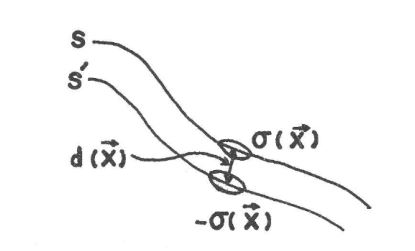
\includegraphics[width=0.75\textwidth]{classical_electrodynamics/img/ch1/1.5.JPG} % first figure itself
         \caption{}
    \end{minipage}
    \begin{minipage}{0.45\textwidth}
        \centering
        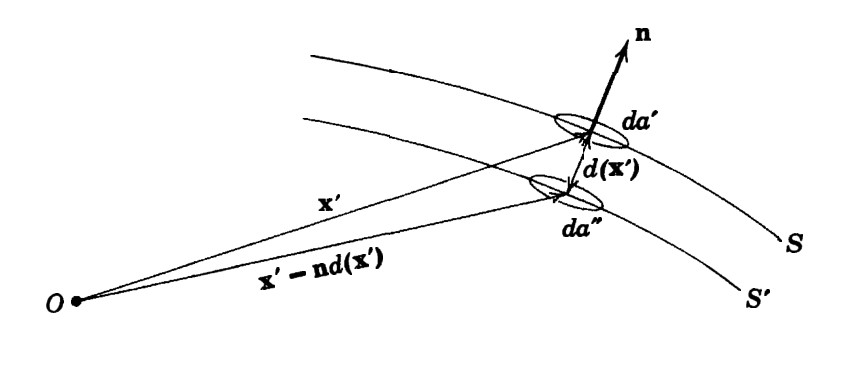
\includegraphics[width=1.1\textwidth]{classical_electrodynamics/img/ch1/1.6.JPG} % second figure itself
       {Dipol-tabaka geometrisi.}
    \end{minipage}
\end{figure}
İlgileneceğimiz bir başka problem ise, bir S yüzeyi üzerindeki bir dipol tabakası dağılımının oluşturduğu potansiyeldir. Şekil 1.5'te gösterildiği gibi, yüzeysel yük yoğunluğu $\sigma(\Vec{x})$ olan bir $S$ yüzeyinin iyice yakınına eşit ve zıt yük yoğunluklu başka bir $S'$ yüzeyi getirilerek bir dipol tabakasının oluşturulduğu düşünülebilir. Dipol dağılımının $D(\Vec{x})$ ile gösterilen şiddetini tanımlamak için  $S'$ yüzeyi  $S$'ye sonsuz küçük derecede yaklaştırılırken  $\sigma(\Vec{x})$ yüzeysel yük yoğunluğu sonsuza götürülür.
\begin{theorem}
$S $ ve $S'$ yüzeyleri bir dipol tabaka oluştursun. Her 2 tabaka eşit ancak zıt yüklü yüzeysel yük yoğunluğuna sahip olsun. Dipol tabakasından kaynaklanan potansiyeli bulmak istiyoruz. Burada $d(\vec{x})$ tabakalar arasındaki mesafedir. Öyle ki bu iki tabaka birbirine sonsuz küçük yaklaşsın yani aralarındaki uzaklık $0$'a gidecek şekilde birbirine son derece yakın hale gelsin. Bu durumda bir tabaka diğer tabakanın yüzeysel yük yoğunluğunu sonsuza götürür.
\[ \lim_{d{(\Vec{x}) \rightarrow 0}} \sigma (\Vec{x}) d (\Vec{x}) = D(\Vec{x}) \]
\[ \sigma = \dfrac{dq}{da} \quad Q = \int_{S} \sigma da \]
Yüzey dipolün dipol-tabaka dağılımı (??)
\[ \phi (\Vec{x}) = k \int \dfrac{\sigma (\Vec{x}')}{|\Vec{x} - \Vec{x}'|} da' \tag{1.23} \]
Şekil 1.6'da görüldüğü gibi, $S$'den $S'$'ne yönelen ve $S$ yüzeyine dik olan birim vektör $\hat{n}$ olmak üzere, bu iki yakın yüzeye ait potansiyel,
\[ \Phi(\Vec{x}) = k  \int_{S} \dfrac{\sigma (\Vec{x}')}{|\Vec{x} - \Vec{x}'|} da' + k \int_{S'} \dfrac{- \sigma (\Vec{x}')}{|\Vec{x} - \Vec{x}' + \hat{n}d|} da'' \]
\[ \Phi(\Vec{x}) = k  \int_{S}  \dfrac{\sigma (\Vec{x}')}{|\Vec{x} - \Vec{x}'|} da' - k \int_{S'} \dfrac{\sigma (\Vec{x}')}{|\Vec{x} - \Vec{x}' + \hat{n}d|} da'' \]
2. terimin Taylor serisini açmamız gerekiyor. İlk olarak genel halini yazalım,
\[ \dfrac{1}{|\Vec{x} + \Vec{a}|} = \dfrac{1}{x} + \Vec{a} \cdot \grad (\dfrac{1}{x}) + \dots \quad |\Vec{a}| \ll |\Vec{x}| \]
\[ \dfrac{1}{|\Vec{x} - \Vec{x'} + \hat{n}d|} = \dfrac{1}{|\Vec{x} - \Vec{x}'|} - d\hat{n} \cdot \dfrac{(\Vec{x} - \Vec{x}')}{|\Vec{x} - \Vec{x'}|^{3}} + \dots \]
\[ \Phi (\Vec{x}) = k \int_{S} \dfrac{\sigma (\Vec{x'})}{|\Vec{x} - \Vec{x'}|} da' - k \Bigg\{ \int_{S} \dfrac{\sigma (\Vec{x'})}{|\Vec{x} - \Vec{x'}|} da'' - \int_{S} \dfrac{(\Vec{x} - \Vec{x'}) \cdot \big[ \sigma (\Vec{x'} ) d\hat{n} \big]}{|\Vec{x} - \Vec{x'}|^{3}} da'' \Bigg\} \]
\dangersign \ 2. ve 3. integralde $S$ yazılmış ama $S'$ olması gerekiyordu??\\
1. integral ve 2. integralin yüzey alanlarını aynı seçersek birbirini götürürler (??).
\[ \lim_{d{(\Vec{x}) \rightarrow 0}} \sigma (\Vec{x}) d (\Vec{x}) = D(\Vec{x}) \textrm{ limitini de uygularsak potansiyel şu şekilde olur,}\]
\[ \Phi (\Vec{x}) = k \int_{S} D(\Vec{x'}) \dfrac{(\Vec{x} - \vec{x}') \cdot \hat{n}}{|\Vec{x} - \Vec{x'}|^{3}} da' \]
\dangersign \ $S'$ ve $da''$ olması gerekmiyor mu??
\[ \Phi (\Vec{x}) = k \int D (\Vec{x}') \dfrac{(\Vec{x} - \Vec{x'}) \cdot \hat{n}}{|\Vec{x} - \Vec{x'}|^{3}} da'\]
$\grad'$'ne göre türev alıyoruz,
\[ \dfrac{\Vec{x} - \Vec{x}'}{|\Vec{x} - \Vec{x}'|^{3}} = \grad ' \Big\{ \dfrac{1}{|\Vec{x} - \Vec{x}'|} \Big\}  \]
\[ \Phi (\Vec{x}) = k \int_{S} D (\Vec{x'}) \hat{n} \cdot \grad ' \Big\{ \dfrac{1}{|\Vec{x} - \Vec{x}'|} \Big\} da' \]
Burada $\Vec{P} = \hat{n} D da$ dipol moment için, $x'$ noktasındaki bir dipolden dolayı $x$ noktasındaki potansiyel,
\[ \phi (\Vec{x}) = k \dfrac{\Vec{P} \cdot (\Vec{x} - \Vec{x'})}{|\Vec{x} - \Vec{x'}|^{3}} \]
Kitapta ekstra olarak, katı açıya bağlı olarak $S$ yüzeyi üzerinden integralini alarak da tanımlamış, (yüzey alanını gören katı açı)
\[ \hat{n} \cdot \grad' \Big( \dfrac{1}{|\Vec{x} - \Vec{x'}|} \Big) da' = - \dfrac{\cos \theta da'}{|\Vec{x} - \Vec{x'}^{2}|} = -d \Omega\]
Burada $d \Omega$ gözlem noktasından $da'$ yüzey elemanını gören katı açı elemanıdır.
\[\Phi (\vec{x}) = -k \int_{S} D (\Vec{x'}) d \Omega \tag{1.26}\]
Bu şekilde bir çift dipol tabakayı geçerken (dipol) potansiyelde bir süreksizlik vardır. 
\[ \Phi_{2} - \Phi_{1} = \dfrac{D}{\varepsilon_{0}} \tag{1.27} \]
%\[D = \sigma d \rightarrow \dfrac{C}{m^{2}} m = \dfrac{C}{m} \]
\end{theorem}

\ 

Bir dipol tabakasını geçerken potansiyelde bir süreksizlik vardır. Bu durum, gözlem noktasını dipol tabakaya sonsuz küçük derecede yaklaştırılarak görülebilir. Bu durumda, gözlem noktasının tam altında olan küçük bir disk ile geri kalan parça olmak üzere, çift tabakasının iki parçadan oluştuğu düşünülebilir. Disk öylesine küçük alınabilir ki, yeterince düz olduğu ve sabit bir D yüzeysel dipol momenti dağılımına sahip olduğu kabul edilebilir. Diskin potansiyeliyle geri kalan kısmının potansiyelinin üst-üste getirilmesiyle toplam potansiyelin elde edilebileceği açıktır. Sadece diskin potansiyeli, iç yüzden dış yüze geçerken $D/\varepsilon_{0}$'lık bir süreksizliğe sahiptir; çünkü Denklem (1.26)'dan açıkça görülebileceği gibi, potansiyel iç yüzde $-D/2\varepsilon_{0}$, dış yüzde ise  $+D/2\varepsilon_{0}$'dır. Diskin çıkarıldığı bir boşluğu bulunan geri kalan parçanın kendi başına potansiyeli, boş kısımdan geçerken süreklidir. Sonuç olarak yüzeyi geçerken potansiyeldeki atlama:
\[ \Phi_{2} - \Phi_{1} = \dfrac{D}{\varepsilon_{0}} \tag{1.27} \]
kadardır. Bu sonuç, bir yüzeysel yük dağılımını geçerken elektrik alandaki süreksizliği gösteren Denklem (\ref{Denklem (1.22)})'nin benzeridir. Denklem (1.27) "fiziksel açıdan" dipol tabakasının "içinde" meydana gelen bir potansiyel düşmesi olarak yorumlanabilir ve iyi yüzeysek yük tabakası arasındaki alan ile limit alınmadan önceki aralığın çarpımı olarak hesaplanabilir.
\newpage
\subsection{Elektrostatik Potensiyel Enerji}
Bölüm 1.5'te, bir noktasal cismin yükü ile skaler potansiyelin çarpımının potansiyel enerji olarak yorumlanabileceği gösterilmişti. Daha kesin söylemek gerekirse, sonsuzda sıfır olan $\Phi$ skaler potansiyeliyle anlatılan elektrik alanlarının bulunduğu bir bölgede bir $q_{i}$ noktasal yükü sonsuzdan bir $\Vec{x}_{i}$ noktasına getirilirse, yük üzerine yapılan iş (dolayısıyla potansiyel enerji),
\begin{align}
    W_{i} = q_{i} \Phi (\Vec{x}_{i}) \tag{1.47}
\end{align}
şeklinde verilir. $\Phi$ potansiyeli, $\Vec{x}_{j}$ konumlarına yerleşmiş $(n-1)$ tane $q_{j}$ yükü $(j=1,2,...,n-1)$ tarafından oluşturulmuş gibi düşünülebilir. Buna göre,
\begin{align}
    \Phi (\Vec{x_{i}}) = k \sum_{j=1}^{n-1} \dfrac{q_{j}}{|\Vec{x_{i} - \Vec{x_{j}}}|} \tag{1.48}
\end{align}
olarak verilir. Öyle ki $q_{i}$ yükünün potansiyel enerjisi,
\begin{align}
    W_{i} = q_{i} k \sum_{j=1}^{n-1} \dfrac{q_{j}}{|x_{i} - x_{j}|} \tag{1.49}
 \end{align}
 şeklindedir.
\begin{theorem}
\[ W = q \int_{A}^{B} \grad \phi \cdot d\Vec{l} = q (\Phi_{B} - \Phi_{A}) \] 
$q_{2}$ yükünü, $\Vec{x_{2}}$ noktasına getirmek için yapılan iş
\[W_{2} = q_{2} \Phi_{1} (\Vec{x_{2}}) \]
Burada $\Phi_{1} (\Vec{x_{2}})$, $\Vec{x_{2}}$ noktasındaki $q_{1}$ yükünden dolayı oluşan potansiyeldir.
\[ \Phi (\Vec{x}) = k  \sum_{j=1}^{n-1} \dfrac{q_{j}}{|\Vec{x_{i}} - \Vec{x_{j}}|}  \]
\[ W_{2} = k \dfrac{q_{2} q_{1}}{|\Vec{x_{2}} - \Vec{x_{1}}|} \]
\[ W_{2} = k  \sum_{i=1}^{n}  \sum_{j<i} \dfrac{q_{i} q_{j}}{|\Vec{x_{i}} - \Vec{x_{j}}|} \]
i ve j üzerinden sınırlanmamış toplamlar 2'ye bölerek çok daha simetrik bir ifade bulunur, (seride çift katlı toplam olduğu için aynı terimi iki defa yazmamak için 2'ye bölüyoruz)
\[ W_{2} = \dfrac{k}{2}  \sum_{i}  \sum_{j} \dfrac{q_{i} q_{j}}{|\Vec{x_{i}} - \Vec{x_{j}}|} \tag{1.51}\]
$i = j$ terimlerinin (sonsuz "öz-enerji" terimleri) çift toplamda atlandığı bilinmelidir (ref. Jackson.) ??

Sürekli yük dağılımı için integrale dönüşecek, çift katlı integral olmak zorundadır
\[ W = \dfrac{k}{2} \int \int \dfrac{\rho (\Vec{x}) \rho (\Vec{x'})}{|\Vec{x} - \Vec{x'}|} d^{3}x d^{3}x' \tag{1.52}\]
Buradaki integrallerden biri skaler potansiyelin kendisidir. Yerine yazarsak,
\[ W = \dfrac{1}{2} \int \rho (\Vec{x}) \phi (\Vec{x}) d^{3}x \tag{1.53}\]
\end{theorem}
Denklem (1.51), (1.52) ve (1.53), elektrostatik potansiyel enerjiyi yüklerin konumları cinsinden anlatırlar ve dolayısıyla yükler arasındaki etkileşmeleri Coulomb kuvvetleri yoluyla vurgularlar.

\newpage

\begin{theorem}
Yüklerin etrafındaki elektrik alanda depolanan enerji Gauss kanunu kullanılarak da bulunabilir.

\[ \grad \cdot \vec{E} = \dfrac{\rho}{\varepsilon_{0}}\]
Buradan $\rho$'yu çekersek,
\[ \rho = \varepsilon_{0} \grad \cdot \Vec{E} \]
olacaktır. Bu eşitliği Denklem (1.53)'de yerine yazarsak,
\[ W = \dfrac{1}{2} \int ( \varepsilon_{0} \grad \cdot \Vec{E}) \phi (\Vec{x}) d^{3}x = \dfrac{\varepsilon_{0}}{2} \int (\grad \cdot \Vec{E}) \phi (\Vec{x}) d^{3}x  \]
Diverjans için çarpım kuralını yazıp hesaplamak istediğimiz terimi çekersek,
\[ \grad \cdot (\Vec{E} \phi) = (\grad \cdot \Vec{E}) \phi + \Vec{E} \cdot (\grad \phi) \]
\[ (\grad \cdot \Vec{E}) \phi =  \grad \cdot (\Vec{E} \phi) - \Vec{E} \cdot (\grad \phi) \]
\[  W =  \dfrac{\varepsilon_{0}}{2} \int (\grad \cdot \Vec{E}) \phi (\Vec{x}) d^{3}x  \]
Burada çarpım kuralını yerine yazalım,
\[  W =  \dfrac{\varepsilon_{0}}{2} \Big\{  \int (\grad \cdot \Vec{E}) \phi d^{3}x - \int (\Vec{E} \cdot \underbrace{\grad \phi}_{-\Vec{E}})  d^{3}x \Big\}\]
Burada 2. terimi düzenlersek,
\[ - \int \Vec{E} \cdot (-\Vec{E}) d^{3}x = \int |\Vec{E}|^{2}  d^{3}x \]
1. terimi düzenlersek, diverjans teoreminden yüzey integraline geçelim
\[ \int_{V} (\grad \cdot \Vec{E}) \phi  d^{3}x = \int_{S} \phi (\Vec{E} \cdot d\vec{a}) = 0 \quad d\Vec{a} = \hat{n} da\]
Bütün yüzey üzerinden integral aldığımızda sonuç 0 olacaktır. Dolayısıyla yapılan iş,
\[  W =  \dfrac{\varepsilon_{0}}{2} \int_{V} |\Vec{E}|^{2}  d^{3}x \tag{1.54}\]
\[  W =  \dfrac{\varepsilon_{0}}{2}  |\Vec{E}|^{2}  V_{\textrm{hacim}} \Rightarrow \dfrac{W}{V_{h}} = \dfrac{\varepsilon_{0}}{2} |\Vec{E}|^{2} \]
Burada artık $w$ enerji yoğunluğudur,
\[ w = \dfrac{\varepsilon_{0}}{2} |\Vec{E}|^{2} \rightarrow \dfrac{\text{Joule}}{\text{m}^{3}} \tag{1.55}  \]
\dangersign \ Burada problem 1.1 ve 1.3 örnek olarak çözülmüştür ama bu çözümleri problemler kısmında vereceğim.
\end{theorem}

Denklem (1.55)'de şaşırtıcı bir nokta vardır. Enerji yoğunluğu pozitif belirlidir. Sonuç olarak, bunun hacim integralinin negatif olmaması gerekir. Bu ise Denklem (1.51)'den edindiğimiz ters işaretli iki yükün potansiyel enerjisinin negatif olacağı izlenimiyle çelişir gibi görünmektedir. Görünüşteki bu çelişkinin nedeni şudur: Denklem (1.54) ve Denklem (1.55), enerji yoğunluğuna öz-enerji katkılarını kapsamakta, oysa Denklem (1.51)'de çift toplam bu katkıları kapsamamaktadır.

\newpage
\subsection{İletken ve Sığa}
\begin{theorem}
    N tane iletkenden oluşan bir sistemimiz olsun. Bu sistem elektrostatik olarak izole olsun. İletkenin içinde elektrik alan 0 olursa potansiyel tüm iletken boyunca sabittir. Böyle yüzeylere eş potansiyel yüzey denir. (+Q, -Q)

\[ \phi_{21} = - \int_{A}^{B} \Vec{E} \cdot d\Vec{l}, \quad C=\dfrac{Q}{V} \]
Q yükü olan tek bir iletkenin kapasitansını bulalım.
\[ W = \dfrac{1}{2} \rho (\Vec{x}) \phi (\Vec{x}) d^{3}x \]
\[= \dfrac{1}{2} \int_{n} \sum_{i=1}^{n} \rho (\Vec{x}) \phi_{i} \Vec{x} d^{3}x  \]
\[W = \dfrac{1}{2} \sum_{i=1}^{n} \phi_{i} \underbrace{\int \rho (\Vec{x})  d^{3}x}_{Q} = \dfrac{1}{2}  \sum_{i=1}^{n} \phi_{i} Q_{i} \]
\[ = \dfrac{1}{2}  \sum_{i=1}^{n} \phi_{i} Q_{i} \]
\[ \phi_{i} = \sum_{j=1}^{n} P_{ij} Q_{j} \quad i=1,2,\dots,n \]
Burada $\phi_{i}$ sütun matrisi, $P_{ij}$ katsayı, $Q_{j}$ sütun matrisidir. $P_{ij}$, tüm yük ve potansiyelleri birbirine bağlar. $P_{ij}$ iletkenin geometrisine bağlıdır. Buna potansiyellerin katsayıları denir.
\[ Q_{i} = \sum_{j=1}^{n} C_{ij} Q_{j  \quad i=1,2,\dots,n } \tag{1.61} \]
C'nin diyagonal elemanları sığa, diyagonal olmayan elemanları elektrostatik indüksiyon katsayısı olarak adlandırılır.
\[ W = \dfrac{1}{2} \sum_{i=1}^{n} Q_{i} \phi_{i} = \dfrac{1}{2} \sum_{i=1}^{n} \sum_{j=1}^{n} C_{ij} Q_{i} Q_{j} \tag{1.62}\]
\dangersign \ Burada kitapta $\phi$ yerine $V$ kullanılmıştır. Ya da notlarda bir sıkıntı var 1.61'de farklı yazılmış.
\[ \begin{pmatrix}
Q \\ -Q  
\end{pmatrix} =  \begin{pmatrix}
C_{11} & C_{12} \\
C_{21} & C_{22}
\end{pmatrix} + \begin{pmatrix}
\phi_{1} \\ \phi_{2}  
\end{pmatrix}  \]
\end{theorem}



\section{Green Teoremi ve Green Fonksiyonları}

\dangersign \ Bu bölüm başlığı, alt bölümlerin düzenlenmesi ve karışıklığa neden olmaması için açılmıştır.

\subsection{Laplace ve Poisson Denklemlerinin Çözümlerinin Tekilliği ve Green Teoremi}

\begin{theorem}
\subsubsection{Sınır Koşulları}
\[ \nabla^{2} \phi = - \dfrac{\rho}{\varepsilon_{0}} \quad \textrm{(Poisson)} \]
\[ \nabla^{2} \phi = 0 \quad \textrm{(Laplace)} \]
Burada tüm problemimiz $\phi$'yi bulmaktır. 

\

Tek boyutta $\dfrac{d^{2} \phi}{dx^{2}} = \lambda, \ x \ \in \ [0,L], \ \lambda \rightarrow \textrm{sabit}$
\[ \phi (x) = \dfrac{1}{2} \lambda x^{2} + ax+b\]
a ve b'yi bulabilmek için 2 sınır koşulu gerekir. Bunlar $\phi (0)$ ve $\phi (L)$'dir. 

\

Kapalı bir S yüzeyi ile sınırlandırılmış sonlu bir V hacmi içerisinde Poisson denkleminin çözümünü bulalım. Poisson veya Laplace denkleminin V hacmi içinde tek ve iyi davranışlı olmasını sağlayan sınır koşulları nelerdir?

\

\textbf{a)} Kapalı bir S yüzeyi üzerinde potansiyeli belirlemek için bir koşul,
\[ \phi (x) \Bigg|_{\Vec{x} \in S} = f (x) \]
Potansiyel sınırda tanımlıdır. Bu koşula \textbf{Dirichlet Koşulu} denir.

\ 


\textbf{b)} Yüzey üzerinde her yerde elektrik alanı belirlemek için \textbf{Neumann Koşulu},
\[ \hat{n} \cdot \grad \phi \Bigg|_{\Vec{x} \in S} = g (\Vec{x}) \]
Bu koşullar altında Laplace ve Poisson denklemlerinin çözümlerinin tek olduğunu gösterelim. Green özdeşliklerini türetelim.

\

Sınır koşullarını ele almak için bazı yeni matematiksel araçlar, yani George Green'e (1824) ait özdeslikler ya da teoremler geliştirmek gereklidir. Bunlar diverjans teoreminin basit uygulamaları olarak ortaya çıkarlar.

\

$\Vec{A}$ bir vektör alanı olsun.
\[ \underbrace{\oint_{S} \Vec{A} \cdot \hat{n} ds}_{\textrm{Akı } (i)} = \underbrace{\int_{V} (\grad \cdot \Vec{A}) d^{3}x}_{\textrm{Akı } (ii)} \]
şeklinde ifade edilen diverjans teoremi, kapalı bir S yüzeyi tarafından sınırlanan bir V hacmi içinde tanımlı olan iyi-davranışlı her $\Vec{A}$ vektör alanına uygulanabilir. $\phi$ ve $\psi$ keyfi sabitler olmak üzere,
\[ \Vec{A} = \phi \grad \psi \]
(ii)'de $\Vec{A}$'yı yerine yazalım,
\[ \grad \cdot \Vec{A} = \grad \cdot (\phi \grad \psi) \]
\[ = \phi \nabla^{2} \psi + \grad \phi \cdot \grad \psi \tag{1.32} \]
(i)'de $\Vec{A}$'yı yerine yazalım,
\[ \Vec{A} \cdot \hat{n} = (\phi \grad \psi) \cdot \hat{n} = \phi \dfrac{\partial \psi}{\partial n} \tag{1.33} \]
Denklem (1.32) ve (1.33)'ü diverjans teoreminde yerine koyalım. Bu aslında I. Green Özdeşliğidir,
\[ \oint_{S} \phi \dfrac{\partial \psi}{\partial n} ds = \int_{V} \Big\{ \phi \nabla^{2} \psi + \grad \phi \cdot \grad \psi \Big\} d^{3}x  \Rightarrow \textrm{ I. Green Özdeşliği} \tag{1.34}\]
Denklem (1.34)'de $\phi$ ve $\psi$'yi yer değiştirerek tekrardan yazalım. $\psi \rightarrow \phi$, \ $\phi \rightarrow \psi$,
\[ \oint_{S} \psi \dfrac{\partial \phi}{\partial n} ds = \int_{V} \Big\{ \psi \nabla^{2} \phi + \grad \psi \cdot \grad \phi \Big\} d^{3}x \]
Bu denklemi, Denklem (1.34)'den çıkaralım, burada $\grad \phi \cdot \grad \psi$ terimleri birbirini yok ederler ve böylece II. Green Özdeşliğini ya da \textbf{Green Teoremini} elde ederiz,
\[ \oint_{S} \bigg( \phi  \dfrac{\partial \psi}{\partial n} - \psi  \dfrac{\partial \phi}{\partial n} \bigg) ds = \int_{V} \bigg(  \phi \nabla^{2} \psi  - \psi \nabla^{2} \phi \bigg) d^{3}x  \Rightarrow \textrm{ II. Green Özdeşliği} \tag{1.35}\]
Poisson denkleminin çözümünün Neumann ve Dirichlet koşulları altında tek olduğunu gösterelim. Aynı koşulları sağlayan 2 tane çözüm olsun: $\phi_{1}$ ve $\phi_{2}$
\[ \phi_{1,2} (\Vec{x})  \Bigg|_{\Vec{x} \in S} = f(x) \rightarrow \textrm{ Dirichlet}  \]
\[ \ \ \ \ \dfrac{\phi_{1,2}}{\partial n}  \Bigg|_{\Vec{x} \in S} = g(x) \rightarrow \textrm{ Neumann}  \]
\begin{tcolorbox}
\textbf{Kitap.} Kapalı S sınır yüzeyi üzerindeki Dirichlet ya da Neumann sınır koşulları bulunan bir V hacmi içerisinde (1.28) Poisson denkleminin çözümlerinin tekliğini göstermek istiyoruz. Tersine, aynı sınır koşullarını sağlayan $\phi_{1}$ ve $\phi_{2}$ gibi iki çözümün bulunduğunu varsayalım.
\begin{align*}
 U(\Vec{x}) = \phi_{1} (\Vec{x}) - \phi_{2} (\Vec{x}) \tag{1.37}    
\end{align*} 
\end{tcolorbox}
$f(x)$ ve $g(x)$ sürekli fonksiyonlar $U(\Vec{x}) = \phi_{1} (\Vec{x}) - \phi_{2} (\Vec{x})$ olsun. $\nabla^{2} U (\Vec{x}) = 0$ Laplace denklemini sağlar. Öyle ki,
\[ \textbf{a. } U(\Vec{x}) \Bigg|_{\Vec{x} \in S} = 0 \rightarrow \textrm{ Dirichlet}  \]
\[ \textbf{b. } \  \dfrac{\partial U}{\partial n} \Bigg|_{\Vec{x} \in S} = 0 \rightarrow \textrm{ Neumann} \]
I. Green Özdeşliğinde $\psi = \phi = U $ olsun:
\[ \oint_{S} U \underbrace{\dfrac{\partial U}{\partial n}}_{=0} ds = \int_{V} \Bigg\{  U \underbrace{\nabla^{2} U}_{=0} + \grad U  \cdot \grad U\Bigg\} d^{3}x \tag{1.38}\]
Burada V hacminin içinde $\nabla^{2}U=0$ (Laplace'dan dolayı); S üzerinde ise Dirichlet sınır koşulu için $U=0$, Neumann sınır koşulu içinse $\partial U / \partial n =0$'dır.
\[ \int_{V} |\grad U|^{2} d^{3}x = 0 \Rightarrow \grad U = 0 \Rightarrow u=sbt \]
$\therefore$ Dirichlet sınır koşulu için V hacmi içinde potansiyel sabit olduğundan yani $\phi_{1} = \phi_{2}$ yüzey üzerinde $U=0$'dır ve çözüm tektir.\\
$\therefore$ Neumann koşulu için yüzey üzerinde $\dfrac{\partial U}{\partial n} = 0$ çözüm tektir.
\\
$\therefore$ Sınırda Neumann ve Dirichlet koşulundan yalnızca bir tanesi sağlanır. Aynı anda ikisi sağlanmaz.
\end{theorem}

\

\

\dangersign \ Sonuç olarak diyebiliriz ki, elektrostatik problemleri, sadece kapalı bir sınır yüzeyi (şüphesiz yüzeyin bir kısmı, ya da tümü sonsuzda olabilir) üzerindeki Dirichlet ya da Neumann sınır koşulları tarafından belirtilir.

\newpage


\subsection{Dirichlet veya Neumann Sınır Koşullarına Sahip Poisson Denklemi için Green Fonksiyonları}

\begin{theorem}
    Sınırlı bir S yüzeyi, V hacmi, Laplace, Poisson, Green fonksiyonu ile çözüm bulunur.
\textbf{Uygulama 1:}
        Boş uzayda, boşlukta $G(x,x') = \dfrac{1}{|x-x'|}$ fonksiyonunu kullanarak herhangi bir $x$ noktasındaki elektriksel potansiyeli hesaplayalım.
\[ \phi(\Vec{x'}) = \int \dfrac{\rho (\Vec{x'})}{|\Vec{x} - \Vec{x'}|} d^{3}x = k \int \rho (\Vec{x'}) G_{0} (\Vec{x},\Vec{x'}) d^{3}x \]
$x'$'teki kaynağın varlığında $\Vec{x}$'teki çözümü Poisson denklemi:
\[ \nabla'^{2}  \dfrac{1}{|\Vec{x} - \Vec{x'}|} = -4 \pi \delta (\Vec{x}-\Vec{x'}) \]
Bu denklemin $x=\Vec{x}'$ noktasında çözümü vardır. Onun dışında 0 verir.
\[ \nabla'^{2}   G_{0} (\Vec{x} - \Vec{x'}) = -4 \pi \delta (\Vec{x}-\Vec{x'}) \tag{1.39} \]
\[ \phi ( \Vec{x}) = k \int \rho (\Vec{x'}) G_{0} (\Vec{x},\Vec{x'}) d^{3}x' + \textrm{ yüzey terimi}  \]
II. Green Özdeşliğini ele alalım:
\[ \phi = \Phi,\  \psi = G_{0} (\Vec{x},\Vec{x'}) = \dfrac{1}{|\Vec{x} - \Vec{x}'|} = \dfrac{1}{R} \]
\[ \underbrace{\oint \Bigg\{ \phi \dfrac{\partial \psi}{\partial n'} - \psi \dfrac{\partial \phi}{\partial n'} \Bigg\} da'}_{(i)} = \int \underbrace{\Bigg\{ \phi \nabla^{2} \psi - \psi \nabla^{2} \phi  \Bigg\} d^{3}x'}_{(ii)} \]
\[  (i) \quad \phi \dfrac{\partial \psi}{\partial n'} - \psi \dfrac{\partial \phi}{\partial n'} = \Phi \dfrac{\partial}{\partial n'} \dfrac{1}{R} - \dfrac{1}{R} \dfrac{\partial \Phi}{\partial n'} \]
\[ (ii) \quad \phi \nabla^{2} \psi - \psi \nabla^{2} \phi = \Phi \underbrace{\nabla^{2} \bigg(\dfrac{1}{R} \bigg)}_{ - 4 \pi \delta (\Vec{x} - \Vec{x}')  } - \dfrac{1}{R} \underbrace{\nabla^{2} \Phi}_{-\rho/\varepsilon_{0}} = \Phi 4 \pi \delta (\Vec{x} - \Vec{x}') + \dfrac{\rho}{R \varepsilon_{0}}\]
Denklemde yerine yazalım,
\[ \oint_{S} \Bigg[ \Phi \dfrac{\partial}{\partial n'} \bigg(\dfrac{1}{R} \bigg) - \dfrac{1}{R}  \dfrac{\partial \Phi}{\partial n'} \Bigg] da' = \int_{V}  \Bigg[ - \Phi 4 \pi \delta (\Vec{x} - \Vec{x}') + \dfrac{\rho}{\varepsilon_{0} R} \Bigg]  d^{3}x'\]
\[ \qquad \qquad \qquad \ \qquad = \int_{V} \dfrac{\rho (\Vec{x}') d^{3}x'}{\varepsilon_{0} R} - 4 \pi \Phi (\Vec{x})\]
\[ \phi (\Vec{x}) = k \int \rho (\Vec{x}') \dfrac{1}{R} d^{3}x' + \dfrac{1}{4 \pi} \oint \Bigg[ \dfrac{1}{R}  \dfrac{\partial \Phi}{\partial n'} - \Phi \dfrac{\partial}{\partial n'} \bigg(\dfrac{1}{R} \bigg) \Bigg] da'  \tag{1.36}\]
$S \rightarrow \infty$ iken S yüzeyi üzerindeki potansiyel $\dfrac{1}{R}$ ile hızla azalarak sınır koşullarını ortadan kaldırır.
\[ \oint_{S} \rightarrow 0\]
\[ \Phi (\Vec{x}) = \dfrac{1}{4 \pi \varepsilon_{0}} \int_{V} \dfrac{\rho (\Vec{x}')}{R} d^{3}x'\]
$\therefore$ Yükün olmadığı durumda $\rho = 0$, $\phi (\Vec{x})$ S yüzeyi üzerinde yalnızca $\phi$ ve $\dfrac{\partial \phi}{\partial n}$'e bağlıdır.
\newpage
\textbf{Uygulama 2:}
\[ G (\Vec{x}, \Vec{x}') = \dfrac{1}{|\Vec{x} - \Vec{x}'|} +  F (\Vec{x} , \Vec{x}') \]
F bilinmeyen bir fonksiyondur öyle ki:
\[ \nabla'^{2} G(\Vec{x}, \Vec{x}') = - 4 \pi \delta (\Vec{x} - \Vec{x}') \rightarrow \textrm{ Nokta kaynak}\]
$\Vec{x}$ ve $\Vec{x}' $, V hacminin içinde olmak üzere;\\
$\nabla'^{2} F(\Vec{x}, \Vec{x}') = 0$ denklemini sağlar.
\[ F \rightarrow \textrm{ Laplace denkleminin bir çözümü}\]
\[ G \rightarrow \textrm{ Poisson denkleminin bir çözümü}\]
II. Gren Özdeşliğinden $\phi = \Phi$, $\psi = G(\Vec{x}, \Vec{x}')$ kullanalım:
\[ \oint_{S}  \Bigg\{ \phi \dfrac{\partial \psi}{\partial n'} - \psi \dfrac{\partial \phi}{\partial n'} \Bigg\} da' = \int_{V} \Bigg\{ \phi \nabla^{2} \psi - \psi \nabla^{2} \phi  \Bigg\} d^{3}x' \]
\[ \oint_{S}  \Bigg\{ \Phi \dfrac{\partial}{\partial n'} G_{0} - G_{0} \dfrac{\partial \Phi}{\partial n'} \Bigg\} da' = \int_{V} \Bigg\{ \Phi \nabla^{2} G_{0} - G_{0} \nabla^{2} \Phi  \Bigg\} d^{3}x' \]
Burada $\nabla^{2} G_{0} = - 4 \pi \delta (\Vec{x} - \Vec{x}')$ ve $\nabla^{2} \Phi = - \dfrac{\rho}{\varepsilon_{0}}$ yerine konulursa,
\[ \Phi (\Vec{x}) = \dfrac{1}{4 \pi \varepsilon_{0}} \int_{V} \rho (\Vec{x}') G(\Vec{x}, \Vec{x'}) d^{3}x' + \dfrac{1}{4 \pi} \int \Bigg\{ G (\Vec{x}, \Vec{x}') \dfrac{\partial \Phi (\Vec{x'})}{\partial n'} - \Phi(\Vec{x}') \dfrac{\partial G (\Vec{x}, \Vec{x'})}{\partial n'}  \Bigg\} da' \]


\end{theorem}


\subsection{Dirichlet Sınır Koşuluna Sahip Green Fonksiyonu}

\begin{theorem}
\[ G_{D} (\Vec{x}, \Vec{x'}) = 0 , \ \Vec{x}' \in S \tag{1.43} \]
\[ \Phi (\Vec{x}) = \dfrac{1}{4 \pi \varepsilon_{0} } \int_{V} \rho(\Vec{x'}) G_{D} (\Vec{x}, \Vec{x}') d^{3}x' + \dfrac{1}{4 \pi} \oint_{S} \Phi (\Vec{x'}) \dfrac{\partial G (\Vec{x} , \Vec{x'})}{\partial n'} da' \tag{1.44} \]
Sistemin geometrisine oldukça bağlıdır ve simetri özelliği vardır. $\Vec{x}$ ile $\Vec{x'}$ yer değiştirilebilir.   
\end{theorem}
\subsection{Neumann Sınır Koşuluna Sahip Green Fonksiyonu}
\begin{theorem}
\[ \dfrac{\partial G_{N}(\Vec{x}, \Vec{x'}) }{\partial n'} = 0, \ \Vec{x'} \in S \]
\[  \dfrac{\partial G_{N}(\Vec{x}, \Vec{x'}) }{\partial n'} \Bigg|_{\Vec{x}' \in S}= \dfrac{- 4 \pi}{S} \tag{1.45} \]
\[ \Phi (\Vec{x}) = \mean{ \Phi}_{S} + \dfrac{1}{4 \pi \epsilon_{0}} \int_{V} \rho (\Vec{x'}) G_{N} (\Vec{x}, \Vec{x'}) d^{3}x' + \dfrac{1}{4 \pi} \oint_{S} G_{N} \dfrac{\partial \Phi (\Vec{x}')}{\partial n} da' \tag{1.46}  \]
\[  \mean{ \Phi}_{S} = \dfrac{1}{S} \oint_{S} \Phi (\Vec{x'}) da'\]
\end{theorem}

\dangersign \ Burada $\mean{ \Phi}_{S}$, potansiyelin tüm yüzey üzerinden ortalama değeridir. Alışılagelen Neumann problemi, "dışsal problem" denendir: bu problemde $V$ hacmi, biri kapalı ve sonlu olan, diğeri ise sonsuzda bulunan iki yüzey tarafından sınırlanmaktadır. Bu durumda $S$ yüzey alanı sonsuzdur; dolayısıyla (1.45) sınır koşulu homojen hale gelir ve $\mean{ \Phi}_{S}$ ortalama değeri sıfır olur.

\
Şuna dikkat edelim: Green fonksiyonları, Dirichlet ya da Neumann sınır değerlerinin ayrıntılı yapılarına bağlı olmayan (1.43) ya da (1.45) gibi basit sınır koşullarını sağlarlar. Böyle olsa bile, çoğunlukla $G(\Vec{x}, \Vec{x'})$'nü saptamak, $S$ yüzeyinin biçimine bağlılığı nedeniyle, (eğer temelli olanaksız değilse) oldukça karışıktır. İkinci ve üçüncü bölümlerde böyle problemlerle karşılaşacağız.


\newpage 

\begin{example}[Şekildeki silindirin hacimce yük yoğunluğu verilmiştir. Silindirin üzerindeki toplam yük miktarı nedir?]
\[ \rho = 100 e^{-z} \Big( x^{2} + y^{2} \Big)^{-1/4} \textrm{  Birimi:}  \dfrac{C}{m^{3}} \]
$r=10$ cm, $h=30$ cm

\begin{center}
\tikzset{every picture/.style={line width=0.75pt}} %set default line width to 0.75pt  
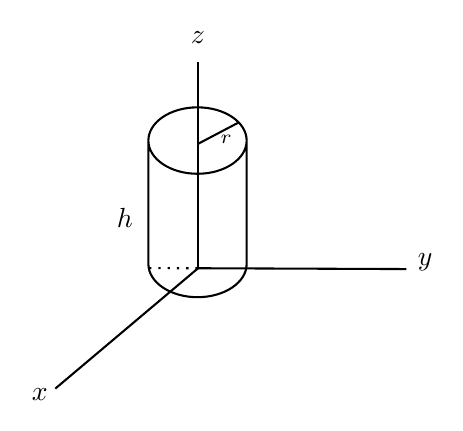
\begin{tikzpicture}[x=0.75pt,y=0.75pt,yscale=-1,xscale=1]
%uncomment if require: \path (0,235); %set diagram left start at 0, and has height of 235
%Straight Lines [id:da43423345815644976] 
\draw    (250.6,51.1) -- (250.6,150.4) ;
%Straight Lines [id:da9928276677292837] 
\draw    (250.6,150.4) -- (181.8,208.4) ;
%Straight Lines [id:da5517329483580377] 
\draw    (250.6,150.4) -- (351,150.8) ;
%Flowchart: Magnetic Disk [id:dp42908362134447153] 
\draw   (274,88.88) -- (274,148.34) .. controls (274,157.18) and (263.4,164.35) .. (250.33,164.35) .. controls (237.25,164.35) and (226.65,157.18) .. (226.65,148.34) -- (226.65,88.88)(274,88.88) .. controls (274,97.72) and (263.4,104.89) .. (250.33,104.89) .. controls (237.25,104.89) and (226.65,97.72) .. (226.65,88.88) .. controls (226.65,80.04) and (237.25,72.88) .. (250.33,72.88) .. controls (263.4,72.88) and (274,80.04) .. (274,88.88) -- cycle ;
%Straight Lines [id:da7590184425073238] 
\draw  [dash pattern={on 0.84pt off 2.51pt}]  (227,150.38) -- (250.6,150.4) ;
%Straight Lines [id:da7520181785921646] 
\draw    (270,80.25) -- (250.75,90.38) ;
% Text Node
\draw (169,207.07) node [anchor=north west][inner sep=0.75pt]    {$x$};
% Text Node
\draw (355,141.73) node [anchor=north west][inner sep=0.75pt]    {$y$};
% Text Node
\draw (245.67,35) node [anchor=north west][inner sep=0.75pt]    {$z$};
% Text Node
\draw (210,120) node [anchor=north west][inner sep=0.75pt]    {$h$};
% Text Node
\draw (260,85) node [anchor=north west][inner sep=0.75pt]  [font=\scriptsize]  {$r$};
\end{tikzpicture}
\end{center}
Silindirde hacimce yük yoğunluğu bilinen bir sistemin toplam yükü nasıl bulunur?
\[ Q= \int \rho dV \]
Silindirik koordinatlarda çözeceğiz soruyu,
\[r^{2} = x^{2} + y^{2}, \quad dV= r dr d\theta dz \]
\[ Q = \int_{r=0}^{0.1} \int_{\theta=0}^{2 \pi}  \int_{z=0}^{0.3} 100 e^{-z} \big\{ r^{2} \big\}^{-1/4} r dr d\theta dz \]
\[ = 100  \int_{0}^{0.1} r^{-1/2} r dr \int_{\theta=0}^{2 \pi}  d\theta \int_{0}^{0.3} e^{-z} dz \]
\[ = 100  \int_{0}^{0.1} r^{1/2}  dr \int_{\theta=0}^{2 \pi}  d\theta \underbrace{\int_{0}^{0.3} e^{-z} dz}_{I_{3}} \]
\begin{tcolorbox}
\[ \Rightarrow I_{3} = \int e ^{-z} dz  \]
\[ u = -z \rightarrow \dfrac{du}{dz} = -1 \rightarrow dz = -du \]
\[  - \int e^{u} du = \dfrac{e^{u}}{ln e} = \dfrac{e^{u}}{1} = - e^{u} \Rightarrow - e^{-z} \]
\[ \Rightarrow I_{3} = - e^{-z} \]
\end{tcolorbox}
\[ = 100  \Bigg\{ \dfrac{2r^{3/2}}{3} \Bigg|_{0}^{0.1} \Bigg\} \Bigg\{ \theta \Bigg|_{0}^{2 \pi} \Bigg\}  \Bigg\{ - e^{-z} \Bigg|_{0}^{0.3} \Bigg\} \]
\[ = 100  \Bigg\{ 0.021 - 0  \Bigg\} \Bigg\{ 2 \pi - 0  \Bigg\}  \Bigg\{ - e^{-0.3} + e^{-0} \Bigg\} = 100  \Bigg\{ 0.021  \Bigg\} \Bigg\{ 2 \pi   \Bigg\}  \Bigg\{ 1 - e^{-0.3} \Bigg\}  \]
\[ = 100  \Bigg\{ 0.021  \Bigg\} \Bigg\{ 2 \pi   \Bigg\}  \Bigg\{ 0.259 \Bigg\} = 3.417 \textrm{ Coulomb} \]
\[ Q = 3.43 \textrm{ Coulomb} \]
\end{example}

\newpage

\begin{example}[$\phi (x) = \dfrac{V_{0}}{2} \big\{ 1 + \dfrac{x}{\sqrt{x^{2} + a^{2}}} \big\} $] 
\[ a \rightarrow \textrm{ eklem bölgesinin genişliği} \]
\[ V_{0} \rightarrow \textrm{ eklem üzerindeki potansiyel fark} \]
Potansiyel Volt biriminde olmalı!
\

\textbf{a)} $\Vec{E} = ?$
\[ E_{x} =  - \dfrac{d \phi}{dx} = - \dfrac{V_{0}}{2} \dfrac{\partial}{\partial x} \Big\{  1 + \dfrac{x}{\sqrt{x^{2} + a^{2}}} \Big\} \]
\[ = - \dfrac{V_{0}}{2} \dfrac{\partial}{\partial x} \Big\{  1 + x (x^{2} + a^{2})^{-1/2}  \Big\}\]
\[ =   - \dfrac{V_{0}}{2}  \Big\{ 1 (x^{2} + a^{2})^{-1/2} - \dfrac{1}{2}  (x^{2} + a^{2})^{-3/2} (2x) x \Big\} \]
\[ =   - V_{0}  \Big\{  \dfrac{1}{\sqrt{x^{2} + a^{2}}} - \dfrac{x^{2}}{(x^{2} + a^{2})^{3/2}} \Big\} \]
\[ =   - V_{0}  \Big\{  \dfrac{(x^{2} + a^{2})}{(x^{2} + a^{2}) \sqrt{x^{2} + a^{2}}} - \dfrac{x^{2}}{(x^{2} + a^{2})^{3/2}} \Big\} \]
\[ =   - V_{0}  \Big\{  \dfrac{(x^{2} + a^{2})}{(x^{2} + a^{2})^{3/2}} - \dfrac{x^{2}}{(x^{2} + a^{2})^{3/2}} \Big\} \]
\[ =   - V_{0}  \Big\{  \dfrac{x^{2} + a^{2} -x^{2}}{(x^{2} + a^{2})^{3/2}} \Big\} = - V_{0}  \Big\{  \dfrac{a^{2}}{(x^{2} + a^{2})^{3/2}} \Big\}  \]
\[ E_{x} = - \dfrac{V_{0} a^{2}}{(x^{2} + a^{2})^{3/2}} \]

\textbf{b)} $\rho$ yük yoğunluğunu bulunuz.

\[ \grad \cdot \Vec{E} = \dfrac{\rho}{\epsilon_{0}} \Rightarrow \rho = \varepsilon_{0} \dfrac{d E_{x}}{dx} \]
\[ \rho = - \varepsilon_{0} V_{0} a^{2} \dfrac{\partial}{\partial x} \Big\{ x^{2} + a^{2} \Big\}^{-3/2} \]
\[ \rho = \dfrac{3}{2} \varepsilon_{0} V_{0} a^{2} 2x \Big\{ x^{2} + a^{2} \Big\}^{-5/2} \]
\[ \rho =  \varepsilon_{0} V_{0} a^{2} \dfrac{3x}{\Big\{ x^{2} + a^{2} \Big\}^{-5/2}} \]
\end{example}


\newpage
\section{Problemler}


\begin{flushleft}
   
\textbf{Soru 1.1:} Gauss teoremini (ve gerekliyse 1.21 denklemini) kullanarak şunları kanıtlayınız:

\

\textbf{a)} Bir iletken üzerine konan her fazlalık yük, tamamıyla iletkenin yüzeyine yayılmalıdır (Bir iletken, tanım gereği, uygulanan elektrik alanlarının etkisi altında serbestçe hareket eden yüklere sahiptir).

\

\textbf{b)} İçi boş kapalı bir iletken kabuk, iç bölgeyi dışardaki yüklerin alanlarına karşı perdeler; fakat dış bölgeyi içeriye konacak yüklerin alanlarına karşı perdeleyemez.

\

\textbf{c)} Bir iletkenin yüzeyindeki elektrik alanı yüzeye dik olup, $\dfrac{\sigma}{\varepsilon_{0}}$ değerine sahiptir; burada $\sigma$ yüzeyin birim alanına düşen yük yoğunluğudur.
\end{flushleft}

  
\textbf{Çözüm:}

\


\textbf{a)} Bir iletkenin içinde $\Vec{E}$ elektrik alanı sıfır olduğu için, Gauss yasası $\grad \cdot \Vec{E} = \dfrac{\rho}{\varepsilon_{0}}$'a göre iletkenin içinde yük yoğunluğu da olmayabilir. Bu sonuç, fazla yükün tamamen yüzeyde olması gerektiği anlamına gelir.

\

\textbf{b)} İletkenin hemen içine bir Gauss yüzeyi yerleştirebilirsiniz. İçeride yük yoğunluğu olmadığı için, Gauss yasasına göre (belki integral formda daha kolay görülür) $\oint \Vec{E} \cdot d\Vec{a} = \dfrac{Q_{\textrm{iç}}}{ \varepsilon_{0}}$ iletkenin dışındaki tüm yüklere rağmen içeride de $\Vec{E}$ elektrik alanı yoktur. Ancak içi boş iletkenin içinde yükler varsa, aynı yasa size $Q \neq 0$'ı söyler, yani dışarıdaki alan da sıfır değildir. Bu nedenle, içini dışarıdaki yüklerden korur, ancak dışını içerideki yüklerden korumaz.

\ 


\textbf{c)} İletkenin yüzeyindeki $\Vec{E}$ alanı yüzeye normal (dik) olmalıdır, aksi takdirde yük yüzeyde akacaktır (yükün statik olduğu varsayımını yapıyoruz). Yüke gelince büyüklüğü için Gauss yasasını integral formunda kullanırız:
\begin{align*}
 \oint \Vec{E} \cdot d\Vec{a} = \dfrac{Q_{\textrm{iç}}}{ \varepsilon_{0}}
\end{align*}
Burada, $d{Q_\textrm{iç}} = \sigma \hat{n} \cdot d \Vec{a}$'dır. Çünkü var olan tek yük yüzeydedir. Gauss yasasını tekrar yazalım,
\begin{align*}
\int \Vec{E} \cdot d \Vec{a} = \int \dfrac{\sigma}{\varepsilon_{0}} \hat{n} \cdot d\Vec{a} = \int (\Vec{E - \dfrac{\sigma}{\varepsilon_{0}} \hat{n}}) \cdot d \Vec{a} =0 
\end{align*}
\begin{align*}
    \Vec{E} = \dfrac{\sigma}{\varepsilon_{0}} \hat{n}
\end{align*}


\


\begin{flushleft}

\newpage
\textbf{Soru 1.3:} Dirac-delta fonksiyonunu uygun koordinatlarda kullanarak, aşağıdaki yük dağılımlarını, üç-boyutlu $\rho (\Vec{x})$ yük yoğunlukları olarak ifade ediniz:

\

\textbf{a)} Küresel koordinatlarda, R yarıçaplı küresel bir kabuk üzerine düzgün dağıtılmış bir $Q$ yükü

\

\textbf{b)} Silindirik koordinatlarda, b yarıçaplı küresel bir kabuk üzerine düzgün dağıtılmış bir $\lambda$ yükü.

\end{flushleft}

  
\textbf{Çözüm:}

\textbf{a)} Küresel bir kabuk üzerine düzgün olarak dağılmış Q yükü vardır. Sadece radyal yöndeki değişimi göz önüne alalım. $\theta$ ve $\phi$'den bağımsız olsun.

\begin{center}
\tikzset{every picture/.style={line width=0.75pt}} %set default line width to 0.75pt        
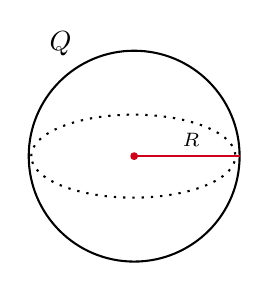
\begin{tikzpicture}[x=0.75pt,y=0.75pt,yscale=-1,xscale=1]
%uncomment if require: \path (0,235); %set diagram left start at 0, and has height of 235

%Shape: Circle [id:dp24624918701902254] 
\draw   (259.4,90.4) .. controls (259.4,62.34) and (282.14,39.6) .. (310.2,39.6) .. controls (338.26,39.6) and (361,62.34) .. (361,90.4) .. controls (361,118.46) and (338.26,141.2) .. (310.2,141.2) .. controls (282.14,141.2) and (259.4,118.46) .. (259.4,90.4) -- cycle ;
%Straight Lines [id:da5047931179893872] 
\draw [color={rgb, 255:red, 208; green, 2; blue, 27 }  ,draw opacity=1 ]   (310.2,90.4) -- (315.8,90.4) -- (361,90.4) ;
\draw [shift={(310.2,90.4)}, rotate = 0] [color={rgb, 255:red, 208; green, 2; blue, 27 }  ,draw opacity=1 ][fill={rgb, 255:red, 208; green, 2; blue, 27 }  ,fill opacity=1 ][line width=0.75]      (0, 0) circle [x radius= 1.34, y radius= 1.34]   ;
%Shape: Ellipse [id:dp7845921950265149] 
\draw  [dash pattern={on 0.84pt off 2.51pt}] (260.6,90.4) .. controls (260.6,79.35) and (282.63,70.4) .. (309.8,70.4) .. controls (336.97,70.4) and (359,79.35) .. (359,90.4) .. controls (359,101.45) and (336.97,110.4) .. (309.8,110.4) .. controls (282.63,110.4) and (260.6,101.45) .. (260.6,90.4) -- cycle ;

% Text Node
\draw (332,78) node [anchor=north west][inner sep=0.75pt]  [font=\scriptsize]  {$R$};
% Text Node
\draw (268,29) node [anchor=north west][inner sep=0.75pt]    {$Q$};
\end{tikzpicture}

\end{center}
\[ \rho (\Vec{x}) \rightarrow \rho (r, \theta, \phi) \]
\[ \rho (r) = A \delta (r - R) = 
\begin{cases}
r=R, & \text{değeri var}\\
r \neq R, & 0
\end{cases}\]
\[ Q = \int \rho dV \Rightarrow \int_{0}^{2 \pi} \int_{0}^{\pi} \int_{0}^{\infty} \rho r^{2} \sin \theta dr d\theta d\phi \]
\[ Q = \int_{0}^{2 \pi} \int_{0}^{\pi} \int_{0}^{\infty} \Big[  A \delta (r - R) \Big] r^{2} \sin \theta dr d\theta d\phi \]
\[ Q = A \int_{0}^{2 \pi} \int_{0}^{\pi} \int_{0}^{\infty} \Big[ \delta (r - R) \Big] r^{2} \sin \theta dr d\theta d\phi \]
\[ Q =  A \int_{0}^{\infty}  \delta (r - R) r^{2} dr  \underbrace{\int_{0}^{\pi} \sin \theta d\theta  \int_{0}^{2 \pi} d \phi}_{4 \pi}\]
\[ Q = 4 \pi A \int_{0}^{\infty}  \delta (r - R) r^{2} dr = 4 \pi A R^{2} \]
$\delta$ fonk. özelliğini kullanarak $r=R$ yazarsak,
\[ Q = 4 \pi A R^{2} \Rightarrow A= \dfrac{Q}{4 \pi R^{2}}\]
\[ \rho (r, \theta, \phi) = \dfrac{Q}{4 \pi R^{2}} \delta (r-R) \]

\textbf{b)} Silindirik koordinatlarda, b yarıçaplı silindirik bir yüzey üzerinde düzgün bir şekilde dağılmış birim uzunluk başına bir $\lambda$ yükü vardır.
\begin{center}
    
\tikzset{every picture/.style={line width=0.75pt}} %set default line width to 0.75pt        

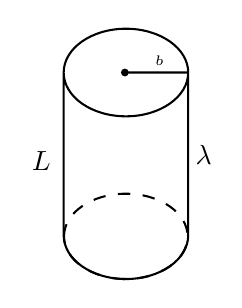
\begin{tikzpicture}[x=0.75pt,y=0.75pt,yscale=-1,xscale=1]
%uncomment if require: \path (0,235); %set diagram left start at 0, and has height of 235

%Flowchart: Magnetic Disk [id:dp6290755443217161] 
\draw   (290.4,56.51) -- (290.4,134.9) .. controls (290.4,146.55) and (276.97,156) .. (260.4,156) .. controls (243.83,156) and (230.4,146.55) .. (230.4,134.9) -- (230.4,56.51)(290.4,56.51) .. controls (290.4,68.16) and (276.97,77.61) .. (260.4,77.61) .. controls (243.83,77.61) and (230.4,68.16) .. (230.4,56.51) .. controls (230.4,44.85) and (243.83,35.4) .. (260.4,35.4) .. controls (276.97,35.4) and (290.4,44.85) .. (290.4,56.51) -- cycle ;
%Shape: Ellipse [id:dp13170873967751273] 
\draw  [dash pattern={on 4.5pt off 4.5pt}][line width=0.75]  (230.56,135.45) .. controls (230.56,124.1) and (243.89,114.9) .. (260.33,114.9) .. controls (276.78,114.9) and (290.11,124.1) .. (290.11,135.45) .. controls (290.11,146.8) and (276.78,156) .. (260.33,156) .. controls (243.89,156) and (230.56,146.8) .. (230.56,135.45) -- cycle ;
%Straight Lines [id:da06796344274943766] 
\draw    (290.4,56.51) -- (259.88,56.5) ;
\draw [shift={(259.88,56.5)}, rotate = 180.01] [color={rgb, 255:red, 0; green, 0; blue, 0 }  ][fill={rgb, 255:red, 0; green, 0; blue, 0 }  ][line width=0.75]      (0, 0) circle [x radius= 1.34, y radius= 1.34]   ;

% Text Node
\draw (213.56,93.07) node [anchor=north west][inner sep=0.75pt]    {$L$};
% Text Node
\draw (292.44,90.18) node [anchor=north west][inner sep=0.75pt]    {$\lambda $};
% Text Node
\draw (273,47.03) node [anchor=north west][inner sep=0.75pt]  [font=\tiny]  {$b$};
\end{tikzpicture}

\end{center}
\[ \rho (\Vec{r}) \rightarrow \rho (r, \theta, z) \]
\[ \rho (r) = A \delta (r - b) = 
\begin{cases}
r=b, & \text{değeri var}\\
r \neq b, & 0
\end{cases}\]
\[ \lambda = \int \rho dV \Rightarrow \int_{0}^{2 \pi} \int_{0}^{\infty} \rho(r) r  dr d\theta \]
\[ \lambda = \int_{0}^{2 \pi} d\theta \int_{0}^{\infty} \Big[  A \delta (r - b) \Big] r  dr  \]
Yük yoğunluğunu normalize ettiğimiz için z üzerinden integral alınmamıştır.
\[ \lambda = 2 \pi A \int_{0}^{\infty} \delta (r - b) r dr \]
$\delta$ fonk. özelliğini kullanarak $r=b$ yazarsak,
\[ \lambda = 2 \pi A b \Rightarrow A = \dfrac{\lambda}{2 \pi b} \]
\[ \rho (r, \theta, z) = \dfrac{\lambda}{2 \pi b}  \delta (r - b)\]
\dangersign \ Bu çözüm notlarda $Q$ yükü üzerinden yapıldığı için, çözümde bir karışıklık vardı. Daha sonra tekrar karşılaştır! \\
\dangersign \ z üzerinden integral alırsak sonuç ne çıkacak???

\newpage


\begin{flushleft}
   
\textbf{Soru 1.4:} a yarıçaplı yüklü üç kürenin her biri toplam Q yüküne sahip olup; biri iletkendir, birinin hacimsel yük yoğunluğu düzgündür, üçüncüsünün ise $r^{n} (n > -3)$ ile değişen küresel simetrik bir yük yoğunluğu vardır. Gauss yasasını kullanarak, her kürenin hem içindeki hem dışındaki elektrik alanlarını bulunuz. İlk iki küre için, yarıçapın fonksiyonu olarak alanların davranışını çiziniz. Aynı çizimi $n=-2$ ve $+2$ halinde üçüncü küre için yapınız.
\end{flushleft}

  
\textbf{Çözüm:}

\[ \oint_{S} \Vec{E} \cdot d \Vec{a} = \dfrac{Q}{\varepsilon_{0}}\]
\

\textbf{a)} 

\begin{center}


\tikzset{every picture/.style={line width=0.75pt}} %set default line width to 0.75pt        

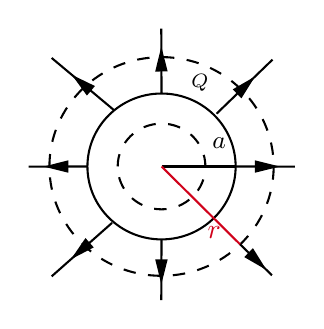
\begin{tikzpicture}[x=0.75pt,y=0.75pt,yscale=-1,xscale=1]
%uncomment if require: \path (0,235); %set diagram left start at 0, and has height of 235

%Flowchart: Connector [id:dp08755890102859121] 
\draw   (208.29,146.5) .. controls (208.29,127.09) and (224.27,111.35) .. (243.99,111.35) .. controls (263.71,111.35) and (279.69,127.09) .. (279.69,146.5) .. controls (279.69,165.91) and (263.71,181.64) .. (243.99,181.64) .. controls (224.27,181.64) and (208.29,165.91) .. (208.29,146.5) -- cycle ;
%Flowchart: Connector [id:dp18147430617386673] 
\draw  [dash pattern={on 4.5pt off 4.5pt}] (189.97,146.5) .. controls (189.97,117.4) and (214.16,93.81) .. (243.99,93.81) .. controls (273.83,93.81) and (298.01,117.4) .. (298.01,146.5) .. controls (298.01,175.59) and (273.83,199.18) .. (243.99,199.18) .. controls (214.16,199.18) and (189.97,175.59) .. (189.97,146.5) -- cycle ;
%Straight Lines [id:da9966891094805954] 
\draw    (243.99,146.5) -- (279.69,146.5) ;
%Straight Lines [id:da9830006170674589] 
\draw [color={rgb, 255:red, 208; green, 2; blue, 27 }  ,draw opacity=1 ]   (243.99,146.5) -- (281.85,184.03) ;
%Straight Lines [id:da3988958838007195] 
\draw    (243.99,111.35) -- (243.86,80.13) ;
\draw [shift={(243.89,88.74)}, rotate = 89.75] [fill={rgb, 255:red, 0; green, 0; blue, 0 }  ][line width=0.08]  [draw opacity=0] (12,-3) -- (0,0) -- (12,3) -- cycle    ;
%Straight Lines [id:da574442204782982] 
\draw    (279.69,146.5) -- (308.25,146.56) ;
\draw [shift={(300.97,146.55)}, rotate = 180.13] [fill={rgb, 255:red, 0; green, 0; blue, 0 }  ][line width=0.08]  [draw opacity=0] (12,-3) -- (0,0) -- (12,3) -- cycle    ;
%Straight Lines [id:da4844285321347075] 
\draw    (208.29,146.5) -- (180,146.56) ;
\draw [shift={(187.15,146.55)}, rotate = 359.87] [fill={rgb, 255:red, 0; green, 0; blue, 0 }  ][line width=0.08]  [draw opacity=0] (12,-3) -- (0,0) -- (12,3) -- cycle    ;
%Straight Lines [id:da8578007645981981] 
\draw    (243.99,181.64) -- (243.86,210.88) ;
\draw [shift={(243.89,203.26)}, rotate = 270.26] [fill={rgb, 255:red, 0; green, 0; blue, 0 }  ][line width=0.08]  [draw opacity=0] (12,-3) -- (0,0) -- (12,3) -- cycle    ;
%Straight Lines [id:da09237587993074259] 
\draw    (270.53,121.05) -- (297.47,95.01) ;
\draw [shift={(289.03,103.16)}, rotate = 135.97] [fill={rgb, 255:red, 0; green, 0; blue, 0 }  ][line width=0.08]  [draw opacity=0] (12,-3) -- (0,0) -- (12,3) -- cycle    ;
%Straight Lines [id:da18127344994441497] 
\draw    (281.85,184.03) -- (297.2,198.92) ;
\draw [shift={(294.55,196.35)}, rotate = 224.1] [fill={rgb, 255:red, 0; green, 0; blue, 0 }  ][line width=0.08]  [draw opacity=0] (12,-3) -- (0,0) -- (12,3) -- cycle    ;
%Straight Lines [id:da021971607148866035] 
\draw    (220.15,173.67) -- (191.05,199.45) ;
\draw [shift={(200.36,191.2)}, rotate = 318.46] [fill={rgb, 255:red, 0; green, 0; blue, 0 }  ][line width=0.08]  [draw opacity=0] (12,-3) -- (0,0) -- (12,3) -- cycle    ;
%Straight Lines [id:da7275627452705213] 
\draw    (221.22,119.46) -- (191.05,94.21) ;
\draw [shift={(200.77,102.34)}, rotate = 39.92] [fill={rgb, 255:red, 0; green, 0; blue, 0 }  ][line width=0.08]  [draw opacity=0] (12,-3) -- (0,0) -- (12,3) -- cycle    ;
%Flowchart: Connector [id:dp40903235672286675] 
\draw  [dash pattern={on 4.5pt off 4.5pt}] (222.86,146.5) .. controls (222.86,135.09) and (232.32,125.84) .. (243.99,125.84) .. controls (255.66,125.84) and (265.12,135.09) .. (265.12,146.5) .. controls (265.12,157.91) and (255.66,167.15) .. (243.99,167.15) .. controls (232.32,167.15) and (222.86,157.91) .. (222.86,146.5) -- cycle ;

% Text Node
\draw (267.02,131.14) node [anchor=north west][inner sep=0.75pt]  [font=\small]  {$a$};
% Text Node
\draw (256.72,100.64) node [anchor=north west][inner sep=0.75pt]  [font=\scriptsize]  {$Q$};
% Text Node
\draw (264.74,174) node [anchor=north west][inner sep=0.75pt]  [color={rgb, 255:red, 208; green, 2; blue, 27 }  ,opacity=1 ]  {$r$};
\end{tikzpicture}

\end{center}
Bütün yük yüzeyde toplanmıştır. İletken bir kürenin içinde elektrik alan 0'dır.
\[ E_{\textrm{iç}} = 0, \ r<a\]
\[ E_{\textrm{dış}} = \dfrac{1}{4 \pi \varepsilon_{0}} \dfrac{Q}{r^{2}}, \ r>a \]
$\Vec{E}$ vektörü radyal yönde, yani $d\Vec{a}$ yüzey elemanı vektörüyle aynı yönde olduğundan, skaler çarpımı kaldırır ve vektörlerin şiddetlerini yazabiliriz,
\[  \oint_{S} \Vec{E} \cdot d\Vec{a} = \oint_{S} |\Vec{E}| da \]
$\Vec{E}$ vektörünün şiddeti Gauss yüzeyi üzerinde her yerde aynı olduğundan, yüzey integrali dışına alınabilir,
\[\oint_{S}  |\Vec{E}| da =  |\Vec{E}| \oint_{S} da =  |\Vec{E}| 4 \pi r^{2} \]
\[  |\Vec{E}| 4 \pi r^{2} = \dfrac{Q}{\varepsilon_{0}} \]
\[  |\Vec{E}|  = \dfrac{1}{4 \pi \varepsilon_{0} }\dfrac{Q}{r^{2}}  \]
\[  \Vec{E}  = \dfrac{1}{4 \pi \varepsilon_{0} }\dfrac{Q}{r^{2}} \hat{r}  \]
\begin{note}[Griffiths]
 Bu sonucun önemli bir özelliğine dikkat edin: Küre dışındaki elektrik alan, merkeze konulan noktasal bir q yükünün alanıyla aynı değerdedir.
\end{note}

\begin{figure}[h!]
\centering
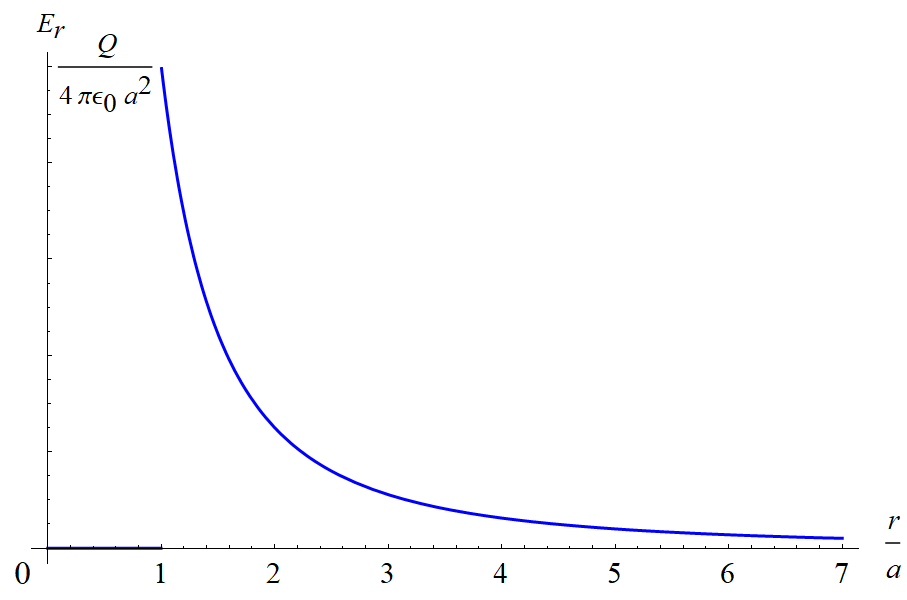
\includegraphics[width=6.5cm]{classical_electrodynamics/img/ch1/1.4.1.png}
\end{figure} 
\newpage
\textbf{b)} Düzgün yük yoğunluğuna sahip küre. Burada kürenin dışındaki çözüm yukarıdaki iletken küre ile aynı miktarda yük içerir ve bu nedenle aynı çözüme sahiptir.

\begin{center}
% Gradient Info
  
\tikzset {_hxh3554c9/.code = {\pgfsetadditionalshadetransform{ \pgftransformshift{\pgfpoint{89.1 bp } { -128.7 bp }  }  \pgftransformscale{1.32 }  }}}
\pgfdeclareradialshading{_463i8c8ys}{\pgfpoint{-72bp}{104bp}}{rgb(0bp)=(1,1,1);
rgb(0bp)=(1,1,1);
rgb(25bp)=(0.26,0.25,0.33);
rgb(400bp)=(0.26,0.25,0.33)}
\tikzset{every picture/.style={line width=0.75pt}} %set default line width to 0.75pt        

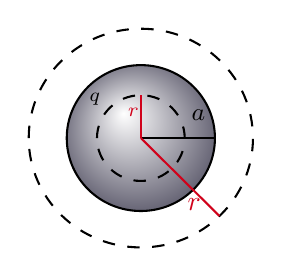
\begin{tikzpicture}[x=0.75pt,y=0.75pt,yscale=-1,xscale=1]
%uncomment if require: \path (0,235); %set diagram left start at 0, and has height of 235

%Flowchart: Connector [id:dp08755890102859121] 
\path  [shading=_463i8c8ys,_hxh3554c9] (208.29,146.5) .. controls (208.29,127.09) and (224.27,111.35) .. (243.99,111.35) .. controls (263.71,111.35) and (279.69,127.09) .. (279.69,146.5) .. controls (279.69,165.91) and (263.71,181.64) .. (243.99,181.64) .. controls (224.27,181.64) and (208.29,165.91) .. (208.29,146.5) -- cycle ; % for fading 
 \draw   (208.29,146.5) .. controls (208.29,127.09) and (224.27,111.35) .. (243.99,111.35) .. controls (263.71,111.35) and (279.69,127.09) .. (279.69,146.5) .. controls (279.69,165.91) and (263.71,181.64) .. (243.99,181.64) .. controls (224.27,181.64) and (208.29,165.91) .. (208.29,146.5) -- cycle ; % for border 

%Flowchart: Connector [id:dp18147430617386673] 
\draw  [dash pattern={on 4.5pt off 4.5pt}] (189.97,146.5) .. controls (189.97,117.4) and (214.16,93.81) .. (243.99,93.81) .. controls (273.83,93.81) and (298.01,117.4) .. (298.01,146.5) .. controls (298.01,175.59) and (273.83,199.18) .. (243.99,199.18) .. controls (214.16,199.18) and (189.97,175.59) .. (189.97,146.5) -- cycle ;
%Straight Lines [id:da9966891094805954] 
\draw    (243.99,146.5) -- (279.69,146.5) ;
%Straight Lines [id:da9830006170674589] 
\draw [color={rgb, 255:red, 208; green, 2; blue, 27 }  ,draw opacity=1 ]   (243.99,146.5) -- (281.85,184.03) ;
%Flowchart: Connector [id:dp40903235672286675] 
\draw  [dash pattern={on 4.5pt off 4.5pt}] (222.86,146.5) .. controls (222.86,135.09) and (232.32,125.84) .. (243.99,125.84) .. controls (255.66,125.84) and (265.12,135.09) .. (265.12,146.5) .. controls (265.12,157.91) and (255.66,167.15) .. (243.99,167.15) .. controls (232.32,167.15) and (222.86,157.91) .. (222.86,146.5) -- cycle ;
%Straight Lines [id:da9419839940961825] 
\draw [color={rgb, 255:red, 208; green, 2; blue, 27 }  ,draw opacity=1 ]   (243.99,146.5) -- (243.99,125.84) ;

% Text Node
\draw (267.02,131.14) node [anchor=north west][inner sep=0.75pt]  [font=\small]  {$a$};
% Text Node
\draw (264.99,174) node [anchor=north west][inner sep=0.75pt]  [color={rgb, 255:red, 208; green, 2; blue, 27 }  ,opacity=1 ]  {$r$};
% Text Node
\draw (236.24,130.62) node [anchor=north west][inner sep=0.75pt]  [font=\scriptsize,color={rgb, 255:red, 208; green, 2; blue, 27 }  ,opacity=1 ]  {$r$};
% Text Node
\draw (217.75,123.15) node [anchor=north west][inner sep=0.75pt]  [font=\scriptsize]  {$q$};
\end{tikzpicture}
\begin{note}[Giancoli]
 Yük, küre içinde simetrik olarak dağıldığından, bütün noktalardaki elektrik alanı da simetrik olmalıdır. $\Vec{E}$ sadece r'ye bağlıdır ve radyal olarak dışarıya doğru yönelir (veya $Q<0$ ise içe doğru).
\end{note}
\end{center}
Kürenin dışı için,
\[  \oint_{S} \Vec{E} \cdot d\Vec{a} = \oint_{S} |\Vec{E}| da \]
\[\oint_{S}  |\Vec{E}| da =  |\Vec{E}| \oint_{S} da =  |\Vec{E}| 4 \pi r^{2} \]
\[  |\Vec{E}| 4 \pi r^{2} = \dfrac{Q}{\varepsilon_{0}} \]
\[  |\Vec{E}|  = \dfrac{1}{4 \pi \varepsilon_{0} }\dfrac{Q}{r^{2}}  \]
\[  \Vec{E}_{\textrm{dış}}  = \dfrac{1}{4 \pi \varepsilon_{0} }\dfrac{Q}{r^{2}} \hat{r}  \]
Küresel simetrik yük dağılımının dışındaki elektrik alanı, kürenin merkezinde bulunan aynı büyüklükteki nokta yükün alanıyla aynı çıktı. 

\ 

Kürenin içi için ($r<a$), yine Gauss yüzeyi seçiyoruz ve Gauss yüzeyindeki toplam yükü yazacağız. Hacimsel yük yoğunluğu her yerde aynıdır.
\[ \oint_{S} \Vec{E} \cdot d\Vec{a} = \dfrac{q}{\varepsilon_{0}}\]
\[ \rho = \dfrac{Q}{\frac{4}{3} \pi a^{3}} \]
\[ q = \rho \dfrac{4}{3} \pi r^{3} = \Bigg(  \dfrac{Q}{\frac{4}{3} \pi a^{3}} \Bigg) \dfrac{4}{3} \pi r^{3} = Q \dfrac{ r^{3}}{a^{3}} \]
\[  |\Vec{E}| 4 \pi r^{2} = \dfrac{ Q \dfrac{ r^{3}}{a^{3}}}{\varepsilon_{0}} = \dfrac{Q}{\varepsilon_{0}} \dfrac{ r^{3}}{a^{3}} \]
\[  |\Vec{E}| =  \dfrac{1}{4 \pi \varepsilon_{0}}  \dfrac{Q r}{ a^{3} } \Rightarrow \Vec{E}_{\textrm{iç}}  = \dfrac{1}{4 \pi \varepsilon_{0}}  \dfrac{Q r}{ a^{3} } \hat{r}  \]
\[  \Vec{E}_{\textrm{iç}}  = \dfrac{1}{4 \pi \varepsilon_{0}}  \dfrac{Q r}{ a^{3} } \hat{r}  \]
\begin{figure}[h!]
\centering
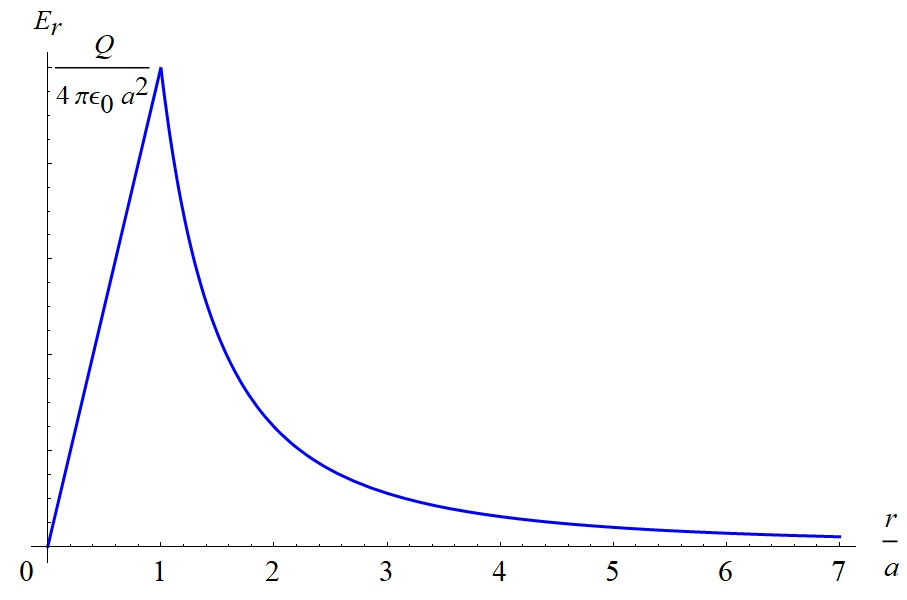
\includegraphics[width=5.5cm]{classical_electrodynamics/img/ch1/1.4.2.jpg}
\end{figure} 

\newpage
\textbf{c)} Kürenin dışı için,
\[  \oint_{S} \Vec{E} \cdot d\Vec{a} = \oint_{S} |\Vec{E}| da \]
\[\oint_{S}  |\Vec{E}| da =  |\Vec{E}| \oint_{S} da =  |\Vec{E}| 4 \pi r^{2} \]
\[  |\Vec{E}| 4 \pi r^{2} = \dfrac{Q}{\varepsilon_{0}} \]
\[  |\Vec{E}|  = \dfrac{1}{4 \pi \varepsilon_{0} }\dfrac{Q}{r^{2}}  \]
\[  \Vec{E}_{\textrm{dış}}  = \dfrac{1}{4 \pi \varepsilon_{0} }\dfrac{Q}{r^{2}} \hat{r}  \]

Kürenin içi için, öncelikle $A$ sabitini bulmamız gerekiyor.
\[ \textrm{Katı kürenin yük yoğunluğu, } \rho = A r^{n} \]
\[ Q = \int \rho dV  = \int_{0}^{a} \int_{0}^{\pi}  \int_{0}^{2 \pi}  A r^{n} r^{2} \sin \theta dr d\theta d \phi \]
\[ Q =  A \int_{0}^{a}  r^{n+2} dr \int_{0}^{\pi} \sin \theta d\theta  \int_{0}^{2 \pi} d \phi \]
\[ =  A  \Bigg\{ \dfrac{r^{n+3}}{n+3} \Bigg|_{0}^{a} \Bigg\} \Bigg\{ - \cos \theta \Bigg|_{0}^{\pi} \Bigg\}  \Bigg\{ \phi \Bigg|_{0}^{2 \pi} \Bigg\} \]
\[ =  A  \Bigg\{ \dfrac{a^{n+3}}{n+3} \Bigg\} \Bigg\{ - \cos \pi + \cos 0 \Bigg\}  \Bigg\{ 2 \pi - 0 \Bigg\} \]
\[ =  A  \Bigg\{ \dfrac{a^{n+3}}{n+3} \Bigg\} \Bigg\{ 1 + 1 \Bigg\}  \Bigg\{ 2 \pi - 0 \Bigg\}  = A  \dfrac{a^{n+3}}{n+3} 4 \pi \]
\[ Q = 4 \pi A \dfrac{a^{n+3}}{n+3} \Rightarrow A = \dfrac{Q (n+3)}{4 \pi a^{n+3}}\]
\[ \rho = \dfrac{Q (n+3)}{4 \pi a^{n+3}} = \dfrac{Q (n+3)}{4 \pi a^{n+3}} r^{n}\]
Kürenin içinde $r$ yarıçaplı Gauss yüzeyi seçelim,
\[ q   = \int_{0}^{r} \int_{0}^{\pi}  \int_{0}^{2 \pi} ( A r^{n} ) r^{2} \sin \theta dr d\theta d \phi \]
\[ q   = \int_{0}^{r} \int_{0}^{\pi}  \int_{0}^{2 \pi} \bigg( \dfrac{Q (n+3)}{4 \pi a^{n+3}} r^{n} \bigg) r^{2} \sin \theta dr d\theta d \phi \]
\[ q   = \bigg( \dfrac{Q (n+3)}{4 \pi a^{n+3}}  \bigg) \int_{0}^{r} r^{n+2} dr \underbrace{\int_{0}^{\pi} \sin \theta d\theta  \int_{0}^{2 \pi} d \phi}_{4 \pi}  \]
\[ q   = \bigg( \dfrac{Q (n+3)}{\cancel{4 \pi} a^{n+3}}  \bigg) \cancel{4 \pi} \int_{0}^{r} r^{n+2} dr  = \bigg( \dfrac{Q (n+3)}{ a^{n+3}}  \bigg) \dfrac{r^{n+3}}{n+3}  \]
\[ q   = Q \dfrac{r^{n+3}}{a^{n+3}} \]
\[ \oint \Vec{E} \cdot d\Vec{a} = \dfrac{\sum q_{\textrm{iç}}}{\varepsilon_{0}}  \]
Burada $\sum q_{\textrm{iç}}$ seçtiğimiz Gauss yüzeyinin içindeki toplam yük miktarıdır,
\[ E (r) \cdot 4 \pi r^{2} = \dfrac{1}{\varepsilon_{0}}  Q \dfrac{r^{n+3}}{a^{n+3}} = \dfrac{1}{4 \pi \varepsilon_{0}}  \dfrac{Q}{r^{2}} \dfrac{r^{n+3}}{a^{n+3}} \]
$r=a$ için, 
\[ E (r) = \dfrac{1}{4 \pi \varepsilon_{0}}  \dfrac{Q}{a^{2}} \]
\begin{flushleft}

   
\textbf{Soru 1.5:} Yüksüz hidrojen atomunun zaman-ortalamalı potansiyeli,
\[ \Phi =\dfrac{q}{4 \pi \varepsilon_{0}}\dfrac{e^{-\alpha r}}{r} (1 + \dfrac{\alpha r}{2})\]
şeklinde verilmektedir. Burada $q$ elektronun yükü ve $\alpha^{-1} = a_{0} / 2$ olup, $a_{0}$ Bohr yarıçapıdır. Bu potansiyeli verecek yük dağılımını (sürekli ve kesikli) bulunuz ve sonucunu fiziksel olarak yorumlayınız.
\end{flushleft}

  
\textbf{Çözüm:}
Elektriksel potansiyelden $\rho$'ya geçmek için,
\[ \nabla^{2} \phi = - \dfrac{\rho}{\varepsilon_{0}} \]
Küresel koordinatlarda laplasyeni yazarsak,
\[ \dfrac{1}{r^{2}} \dfrac{\partial }{\partial r} \Big\{ r^{2}   \dfrac{\partial \phi}{\partial r} \Big\} + \dfrac{1}{r^{2} \sin \theta }  \dfrac{\partial}{\partial \theta} \Big\{  \sin \theta \cancelto{0}{\dfrac{\partial \phi}{\partial \theta}} \Big\}  + \dfrac{1}{r^{2} \sin^{2} \theta} \cancelto{0}{\dfrac{\partial^{2} \phi}{\partial \varphi^{2}}} = -  \dfrac{\rho}{\varepsilon_{0}} \]
\[  \dfrac{1}{r^{2}} \dfrac{\partial}{\partial r} \Big\{ r^{2}   \dfrac{\partial \phi}{\partial r} \Big\}  = -  \dfrac{\rho}{\varepsilon_{0}} \]
\[  \dfrac{1}{r^{2}} \dfrac{\partial}{\partial r} \Bigg\{ r^{2}   \dfrac{\partial}{\partial r} \Big[ \dfrac{1}{4 \pi \varepsilon_{0}} \dfrac{e^{- \alpha r}}{r} (1 + \dfrac{\alpha r}{2})\Big] \Bigg\}  = -  \dfrac{\rho}{\varepsilon_{0}} \]
\[ \dfrac{1}{4 \pi \varepsilon_{0}}  \dfrac{1}{r^{2}} \dfrac{\partial}{\partial r} \Bigg\{ r^{2}   \dfrac{\partial}{\partial r} \Big[ \dfrac{e^{- \alpha r}}{r} (1 + \dfrac{\alpha r}{2})\Big] \Bigg\}  = -  \dfrac{\rho}{\varepsilon_{0}} \]
%\[ \dfrac{\partial}{\partial r} \Big[ \dfrac{e^{- \alpha r}}{r} (1 + \dfrac{\alpha r}{2})\Big] =  \]
\dangersign \ Ara işlemi siz yapın!
\[ \Rightarrow - \dfrac{1}{4 \pi r^{2}} \dfrac{\partial}{\partial r} \Big\{ \alpha r E^{- \alpha r} + e^{- \alpha r} + \dfrac{\alpha^{2}}{2} r^{2} e^{- \alpha r}  \Big\} = -\rho \]
\[ \rho = - \dfrac{1}{8 \pi} \alpha^{3} e^{- \alpha r}\]
\[ e^{- \alpha r} = 1 \textrm{ alırsak,} \]
\[ \phi (r) = \dfrac{1}{4 \pi \varepsilon_{0}} \dfrac{q}{r} +  \dfrac{1}{4 \pi \varepsilon_{0}} \dfrac{q \alpha}{2} \]
2. terimdekiler sabit olduğu için $\phi (r)$'yi yaklaşık şöyle alabilirim,
\[ \phi(r) = \dfrac{1}{4 \pi \varepsilon_{0}} \dfrac{q}{r} \]
Şimdi Poissonu uygulayabiliriz,
\[ \nabla^{2} \phi = - \dfrac{\rho}{\varepsilon_{0}} \]
\[ kq \nabla^{2} (\dfrac{1}{r}) =  - \dfrac{\rho}{\varepsilon_{0}} \]
Burada,
\[ \nabla^{2} (\dfrac{1}{r}) = - 4 \pi \delta (r) \textrm{'dir.} \]
\[ kq \big(  - 4 \pi \delta(r) \big) = - \dfrac{\rho}{\varepsilon_{0}} \]
\[  \dfrac{q}{\cancel{4 \pi} \varepsilon_{0}}  \cancel{4 \pi} \delta(r) = \dfrac{\rho}{\varepsilon_{0}} \]
\[ \rho = q  \delta(r)\]
\[ \rho = - \dfrac{q}{ 8 \pi} \alpha^{3} e^{- \alpha r} + q \delta (r)\]
\dangersign \ Buna tekrar bak!
\newpage
\begin{flushleft}
   
	\textbf{1.14} Consider the electrostatic Green functions of Section 1.10 for Dirichlet and Neumann boundary conditions on the surface S bounding the volume V. Apply Green's theorem (1.35) with integration variables $\Vec{y}$ and $\phi = G(\Vec{x},\Vec{y})$, $\psi = G (\vec{x}', \Vec{y})$, with $\nabla^{2}_{y}G(\Vec{z},\Vec{y}) = -4\pi \delta  (\Vec{y}-\Vec{z})$. Find an expression for the difference $[ G(\Vec{x} ,\vec{x}' ) - G ( \vec{x}' , \Vec{x} )]$ in terms of an integral over the boundary surface S. 

\

\textbf{a)} For Dirichlet boundary conditions on the potential and the associated boundary condition on the Green function, show that $G_{D}(\Vec{x},\vec{x}') $	must be symmetric in $\Vec{x}$ and $\vec{x}'$.

\

\textbf{b)} For Neumann boundary conditions, use the boundary condition (1.45) for $G_{N} = ( \Vec{x} , \vec{x}')$ to show that $G_{N} = ( \Vec{x} , \vec{x}')$ is not symmetric in general, but that $G_{N} = ( \Vec{x} , \vec{x}') - F (\Vec{x})$ is symmetric in $\Vec{x}$ and $\vec{x}'$, where

\begin{align*}
    F (x) = \dfrac{1}{S} \oint_{S} G_{N} ( \Vec{x}, \Vec{y} ) da_{y}
\end{align*}

\

\textbf{c)} Show that the addition of $F(\Vec{x})$ to the Green function does not affect the potential $\phi(\Vec{x})$. See problem 3.26 for an example of the Neumann Green function.	
\end{flushleft}

  
\textbf{Çözüm:}

\

\textbf{a)}
\begin{align*}
  \phi ( \Vec{x}) =  \dfrac{1}{4 \pi \epsilon_{0}} \int_{V} \rho ( \vec{x}' )  G( \Vec{x} ,\vec{x}' ) d^{3} x' + \dfrac{1}{4 \pi} \oint \Bigg\{ G \dfrac{\partial \phi}{\partial n'} - \phi \dfrac{\partial G}{\partial n'}  \Bigg\} da'  
\end{align*}
\begin{align*}
\int_{V} \Bigg\{ \phi \nabla^{2} \psi - \psi \nabla^{2} \phi  \Bigg\} d^{3} y = \oint_{S} \Bigg\{  \phi \dfrac{\partial \psi}{\partial n} - \psi \dfrac{\partial \phi}{\partial n}\Bigg\} d a_{y}
\end{align*}

\begin{tcolorbox}
\begin{align*}
\phi = G ( \Vec{x}, \Vec{y}) \qquad \psi = G ( \vec{x}', \Vec{y})    
\end{align*}
\begin{align*}
\nabla^{2}_{y} G ( \Vec{z}, \Vec{y} ) = - 4 \pi \delta (\Vec{y} - \Vec{z}) 
\end{align*}
\end{tcolorbox}
\begin{align*}
\int_{V} \bigg\{  G (\Vec{x}, \Vec{y}) \begingroup \color{blue}{ \underbrace{\nabla^{2}_{y} G ( \vec{x}', \Vec{y} )}_\text{$-4\pi \delta (\Vec{y} - \vec{x}')$} } \endgroup  - G ( \vec{x}', \Vec{y} ) \begingroup \color{blue}{ \underbrace{\nabla^{2}_{y} G ( \vec{x}, \Vec{y} )}_\text{$-4\pi \delta (\Vec{y} - \vec{x})$} } \endgroup  \bigg\} d^{3} y = \oint_{S} \bigg\{ G ( \Vec{x} , \Vec{y}  ) \dfrac{\partial G (\vec{x}', \Vec{y} )}{\partial n} - G ( \vec{x}', \Vec{y} ) \dfrac{\partial G ( \Vec{x}, \Vec{y} )}{\partial n} \bigg\} da_{y} 
\end{align*}
\begin{align*}
-4 \pi \int_{V} G ( \Vec{x}, \Vec{y}) \delta ( \Vec{y} - \vec{x}') - G ( \vec{x}' , \Vec{y}) \delta ( \Vec{y} - \vec{x}) d^{3} y  = \oint_{S} \bigg\{ G ( \Vec{x} , \Vec{y}  ) \dfrac{\partial G (\vec{x}', \Vec{y} )}{\partial n} - G ( \vec{x}', \Vec{y} ) \dfrac{\partial G ( \Vec{x}, \Vec{y} )}{\partial n} \bigg\} da_{y} 
\end{align*}
\begin{align*}
-4 \pi \bigg\{ G (\Vec{x}, \vec{x}') - G (\vec{x}', \Vec{x} ) \bigg\} = \oint_{S} \bigg\{ G ( \Vec{x} , \Vec{y}  ) \dfrac{\partial G (\vec{x}', \Vec{y} )}{\partial n} - G ( \vec{x}', \Vec{y} ) \dfrac{\partial G ( \Vec{x}, \Vec{y} )}{\partial n} \bigg\} da_{y} 
\end{align*}
\begin{align*}
G (\Vec{x}, \vec{x}') - G (\vec{x}', \Vec{x} ) = - \dfrac{1}{4 \pi} \oint_{S} \bigg\{ G ( \Vec{x} , \Vec{y}  ) \dfrac{\partial G (\vec{x}', \Vec{y} )}{\partial n} - G ( \vec{x}', \Vec{y} ) \dfrac{\partial G ( \Vec{x}, \Vec{y} )}{\partial n} \bigg\} da_{y} 
\end{align*}

\newpage


Dirichlet sınır koşulu S yüzeyinde $G_{D} (\Vec{x}, \Vec{y}) = 0$ olduğu anlamına gelmektedir. Bu, tüm yüzey integralinin sıfır olduğu anlamına gelir ve $G_{D}$'nin $(\Vec{x}$ ve $\vec{x}')$'ünde simetrik olduğunu gösterir.

\begin{align*}
G_{D} (\Vec{x}, \vec{x}') = 0
\end{align*}
\begin{align*}
\phi (\Vec{x}) \dfrac{1}{4 \pi \epsilon_{0}} \int_{V} \rho (\vec{x}') G_{D} (\Vec{x}, \vec{x}') d^{3} x' - \dfrac{1}{4 \pi} \oint_{S} \phi \dfrac{\partial G_{D}}{\partial n'} da'
\end{align*}
\begin{align*}
G (\Vec{x}, \vec{x}') - G (\vec{x}', \Vec{x} ) = - \dfrac{1}{4 \pi} \oint_{S} \bigg\{ \begingroup \color{blue}{\underbrace{G ( \Vec{x} , \Vec{y}  )}_\text{0}} \endgroup \dfrac{\partial \begingroup \color{blue}{\overbrace{ G (\vec{x}', \Vec{y} )}^\text{0}} \endgroup}{\partial n} -  \begingroup \color{blue}{\underbrace{ G ( \vec{x}', \Vec{y} )}_\text{0}} \endgroup  \dfrac{\partial \begingroup \color{blue}{\overbrace{G ( \Vec{x}, \Vec{y} )}^\text{0}} \endgroup }{\partial n} \bigg\} da_{y} 
\end{align*} 
\begin{align*}
G (\Vec{x}, \vec{x}') - G (\vec{x}', \Vec{x} ) = 0
\end{align*} 
\begin{align*}
G (\Vec{x}, \vec{x}')  = G (\vec{x}', \Vec{x} ) \qed
\end{align*} 
\begin{tcolorbox}
\[
    G_{D}(\Vec{x}, \Vec{x'}), \Vec{x} \textrm{ ve } \Vec{x'}\textrm{'nde açıkça simetriktir.}
\]
\end{tcolorbox}
\textbf{b)}
\begin{tcolorbox}
Neumann sınır koşulu,
\begin{align*}
    \dfrac{\partial G_{N}}{\partial n'} (\Vec{x} - \vec{x}') = - \dfrac{4 \pi}{S} \textrm{  $\Vec{x}$ on $S$}
\end{align*}
\end{tcolorbox}
\begin{align*}
  \phi ( \Vec{x}) =  \dfrac{1}{4 \pi \epsilon_{0}} \int_{V} \rho ( \vec{x}' )  G_{N}( \Vec{x} ,\vec{x}' ) d^{3} x' + \dfrac{1}{4 \pi} \oint_{S}  G_{N}( \Vec{x} ,\vec{x}' ) \dfrac{\partial \phi}{\partial n'}  da' + \mean{\phi}_{S}
\end{align*}
\begin{align*}
G_{N} (\Vec{x}, \vec{x}') - G_{N} (\vec{x}', \Vec{x} ) = - \dfrac{1}{4 \pi} \oint_{S} \bigg\{ G_{N} ( \Vec{x} , \Vec{y}) \begingroup \color{blue}{\underbrace{\dfrac{\partial G_{N} (\vec{x}', \Vec{y} )}{\partial n}}_\text{$\dfrac{-4\pi}{S}$} } \endgroup  - G_{N} ( \vec{x}', \Vec{y} )\begingroup \color{blue}{\underbrace{\dfrac{\partial G_{N} (\vec{x}, \Vec{y} )}{\partial n}}_\text{$\dfrac{-4\pi}{S}$} } \endgroup \bigg\} da_{y} 
\end{align*}
\begin{align*}
G_{N} (\Vec{x}, \vec{x}') - G_{N} (\vec{x}', \Vec{x} ) =  \dfrac{1}{S} \oint_{S} \bigg\{ G_{N} ( \Vec{x} , \Vec{y})  - G_{N} ( \vec{x}', \Vec{y} ) \bigg\} da_{y} 
\end{align*}
\begin{align*}
G_{N} (\Vec{x}, \vec{x}') - \begingroup \color{blue}{\underbrace{ \dfrac{1}{S} \oint_{S} G_{N} ( \Vec{x} , \Vec{y}) da_{y}}_\text{$F(\Vec{x})$} } \endgroup   =  G_{N} (\vec{x}', \Vec{x} ) -\begingroup \color{blue}{\underbrace{ \dfrac{1}{S} \oint_{S} G_{N} ( \vec{x}' , \Vec{y}) da_{y}}_\text{$F(\vec{x}')$} } \endgroup
\end{align*}
\begin{align*}
G_{N} (\Vec{x}, \vec{x}')  - F (\Vec{x})   =  G_{N} (\vec{x}', \Vec{x} )  - F (\vec{x}') \qed
\end{align*}
\begin{tcolorbox}
\centering
Fark simetriktir!
\end{tcolorbox}

\newpage

\textbf{c)}
\begin{align*}
  \phi ( \Vec{x}) =  \dfrac{1}{4 \pi \epsilon_{0}} \int_{V} \rho ( \vec{x}' )  G_{N}( \Vec{x} ,\vec{x}' ) d^{3} x' + \dfrac{1}{4 \pi} \oint_{S}  G_{N}( \Vec{x} ,\vec{x}' ) \dfrac{\partial \phi}{\partial n'}  da' + \mean{\phi}_{S}
\end{align*}

Green fonksiyonuna $F(\Vec{x})$ ekleyerek $\phi (\Vec{x}) $ potansiyeli üzerindeki etkisine bakalım,

\begin{align*}
\phi' ( \Vec{x}) =  \dfrac{1}{4 \pi \epsilon_{0}} \int_{V} \rho ( \vec{x}' ) ( G_{N}( \Vec{x} ,\vec{x}' ) + F(\Vec{x})) d^{3} x' + \dfrac{1}{4 \pi} \oint_{S} ( G_{N}( \Vec{x} ,\vec{x}' ) + F(\Vec{x}) ) \dfrac{\partial \phi}{\partial n'}  da' + \mean{\phi}_{S} 
\end{align*}
\begin{align*}
=  \dfrac{1}{4 \pi \epsilon_{0}} \bigg\{ \int_{V} \rho ( \vec{x}' )  G_{N}( \Vec{x} ,\vec{x}' )  d^{3} x' + \int_{V} \rho ( \vec{x}' )  F(\Vec{x})  d^{3} x' \bigg\} + \dfrac{1}{4 \pi} \bigg\{ \oint_{S} G_{N}( \Vec{x} ,\vec{x}' ) \dfrac{\partial \phi}{\partial n'} da' + \oint_{S} F(\Vec{x})  \dfrac{\partial \phi}{\partial n'}  da' \bigg\} + \mean{\phi}_{S} 
\end{align*}
\begin{align*}
\begin{aligned}
\phi' ( \Vec{x}) & =  \dfrac{1}{4 \pi \epsilon_{0}} \int_{V} \rho ( \vec{x}' )  G_{N}( \Vec{x} ,\vec{x}' )  d^{3} x' + \dfrac{1}{4 \pi \epsilon_{0}} \int_{V} \rho ( \vec{x}' )  F(\Vec{x})  d^{3} x' \\
& \ + \dfrac{1}{4 \pi} \oint_{S} G_{N}( \Vec{x} ,\vec{x}' ) \dfrac{\partial \phi}{\partial n'} da' + \dfrac{1}{4 \pi} \oint_{S} F(\Vec{x})  \dfrac{\partial \phi}{\partial n'}  da'  + \mean{\phi}_{S} 
\end{aligned}
\end{align*}
\begin{align*}
\begin{aligned}
\phi' ( \Vec{x}) & =  \begingroup \color{blue}{\overbrace{ \dfrac{1}{4 \pi \epsilon_{0}} \int_{V} \rho ( \vec{x}' )  G_{N}( \Vec{x} ,\vec{x}' )  d^{3} x' + \dfrac{1}{4 \pi} \oint_{S} G_{N}( \Vec{x} ,\vec{x}' ) \dfrac{\partial \phi}{\partial n'} da'}^\text{$\phi (\Vec{x})$}} \endgroup  \\
& \ + \dfrac{1}{4 \pi \epsilon_{0}} \int_{V} \rho ( \vec{x}' )  F(\Vec{x})  d^{3} x'  + \dfrac{1}{4 \pi} \oint_{S} F(\Vec{x})  \dfrac{\partial \phi}{\partial n'}  da'  + \mean{\phi}_{S} 
\end{aligned}
\end{align*} 
\begin{align*}
\phi' ( \Vec{x}) = \phi (\Vec{x}) + \dfrac{1}{4 \pi \epsilon_{0}} \int_{V} \rho ( \vec{x}' )  F(\Vec{x})  d^{3} x'  + \dfrac{1}{4 \pi} \oint_{S} F(\Vec{x})  \dfrac{\partial \phi}{\partial n'}  da'  
\end{align*} 
\begin{align*}
 = \phi (\Vec{x}) + \dfrac{1}{4 \pi} F(\Vec{x}) \bigg\{ \dfrac{1}{\epsilon_{0}} \int_{V} \rho ( \vec{x}' )  d^{3} x'  + \oint_{S} \dfrac{\partial \phi}{\partial n'}  da' \bigg\}  
\end{align*} 
\begin{tcolorbox}
Gauss yasası,
\begin{align*}
\oint_{S} \Vec{E} \cdot d \Vec{A} = \dfrac{1}{\epsilon_{0}} \int_{V} \rho \cdot dV
\end{align*}
Kullandığımız notasyona göre değişkenler yerine konunca,
\begin{align*}
\oint_{S} \Vec{E} \cdot \Vec{n'} da' = \dfrac{1}{\epsilon_{0}} \int_{V} \rho (\vec{x}') d^{3} x'
\end{align*}
\end{tcolorbox}
\begin{align*}
\phi' ( \Vec{x})  = \phi (\Vec{x}) + \dfrac{1}{4 \pi} F(\Vec{x}) \bigg\{ \oint_{S} \Vec{E} \cdot \Vec{n'} da'   + \oint_{S} \dfrac{\partial \phi}{\partial n'}  da' \bigg\}  
\end{align*} 
\begin{align*}
\phi' ( \Vec{x})  = \phi (\Vec{x}) + \dfrac{1}{4 \pi} F(\Vec{x}) \bigg\{ - \oint_{S} \Vec{\nabla} \phi \cdot \Vec{n'} da'   + \oint_{S} \dfrac{\partial \phi}{\partial n'}  da' \bigg\} 
\end{align*}
\begin{align*}
\dfrac{\partial \phi}{\partial n} = \nabla \phi \cdot \Vec{n} \textrm{  olduğundan},
\end{align*}
\begin{align*}
\phi' ( \Vec{x})  = \phi (\Vec{x}) + \dfrac{1}{4 \pi} F(\Vec{x}) \bigg\{ - \oint_{S} \dfrac{\partial \phi}{\partial n'} da'   + \oint_{S} \dfrac{\partial \phi}{\partial n'}  da' \bigg\}  
\end{align*}
\begin{align*}
\phi' ( \Vec{x})  = \phi (\Vec{x}) + \dfrac{1}{4 \pi} F(\Vec{x}) \bigg\{ 0 \bigg\}  
\end{align*}
\begin{align*}
\phi' ( \Vec{x})  = \phi (\Vec{x}) \qed
\end{align*}
$F(\Vec{x})$'in Green fonksiyonuna eklenmesi $\phi (\Vec{x})$ potansiyelini etkilememektedir.  

\newpage

\section{Ödevler}
\subsection*{Ödev 0}

   \begin{flushleft}
   \begin{align*}
       \epsilon_{0} = 8.8541 \times 10^{-12} \textrm{ F$\cdot$m$^{-1}$}
   \end{align*}
   \begin{align*}
       k = \dfrac{1}{4 \pi \epsilon_{0}} = 8.9875 \times 10^{9} \textrm{ N$\cdot$m$^{2}$$\cdot$C$^{-2}$}
       \end{align*}
   
	\textbf{Soru 1:} $ \phi (x) = \dfrac{V_{0}}{2} \Big( 1 + \dfrac{x}{\sqrt{x^{2}+a^{2}}} \Big) $ \textrm{denkleminin} $\phi(x), E_{x}$ ve $\rho$ için grafiklerini gösteriniz.

	
\end{flushleft}
   
	\textbf{Çözüm:} 

\ 

 \textbf{a)}
 \begin{align}
     E_{x} = - \dfrac{V_{0}a^{2}}{(x^{2} + a^{2} )^{3/2}}
 \end{align}
 \begin{figure}[h]
 \centering
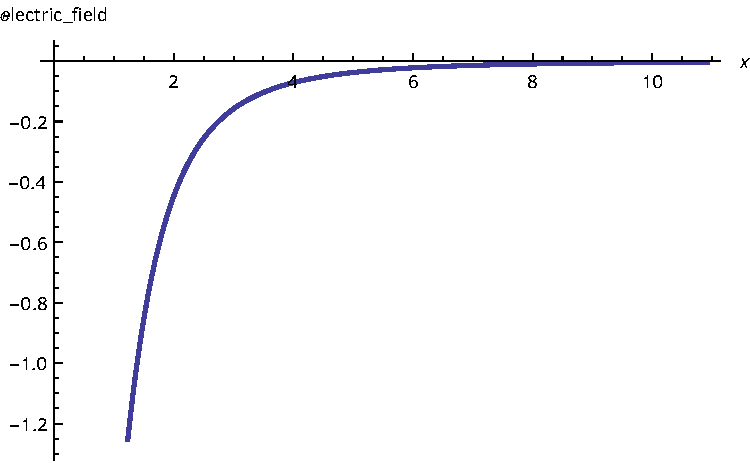
\includegraphics[width=8cm]{classical_electrodynamics/img/ch1/ödev/E_x.pdf}
\caption*{$V_{0} = 5V, a=1$br alınmıştır.}
	\end{figure}
 \begin{figure}[h!]
 \centering
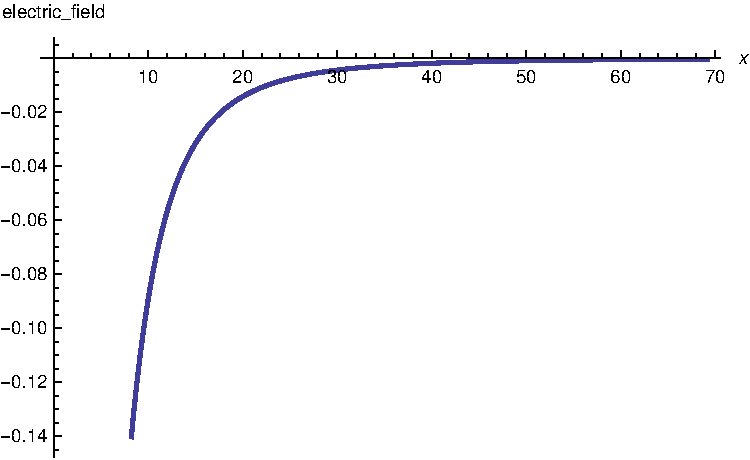
\includegraphics[width=8cm]{classical_electrodynamics/img/ch1/ödev/E_x2.pdf}
\caption*{$V_{0} = 5V, a=5br$ alınmıştır.}
	\end{figure}
\newpage 

 \textbf{b)}
 \begin{align}
     \rho = \dfrac{3}{2}V_{0} a^{2} \epsilon_{0} x (x^{2}+a^{2})^{-\dfrac{5}{2}}
 \end{align}
 \begin{figure}[h]
 \centering
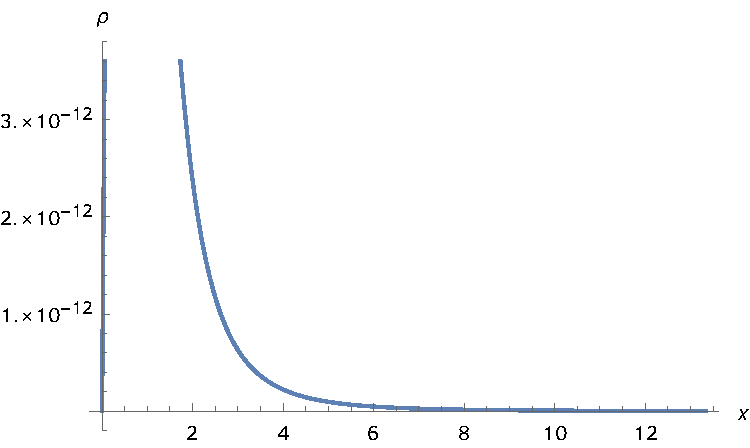
\includegraphics[width=10cm]{classical_electrodynamics/img/ch1/ödev/rho.pdf}
\caption*{$V_{0} = 5V, a=1br$ alınmıştır.}
\end{figure}	
\begin{figure}[h]
 \centering
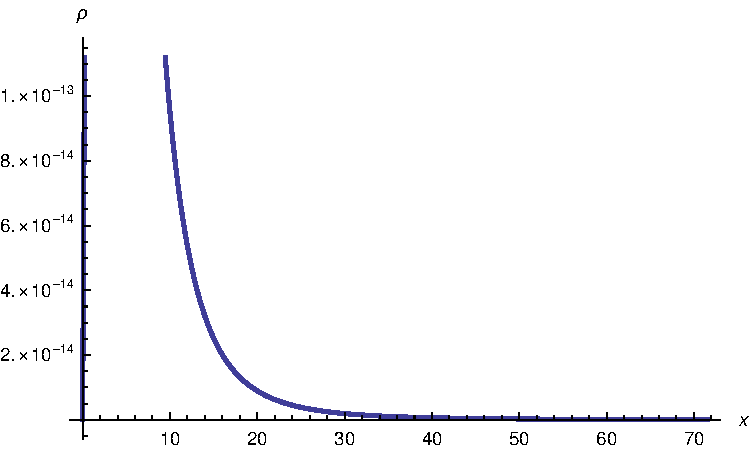
\includegraphics[width=10cm]{classical_electrodynamics/img/ch1/ödev/rho3.pdf}
\caption*{$V_{0} = 5V, a=5br$ alınmıştır.}
\end{figure}
  \begin{figure}[h!]
 \centering
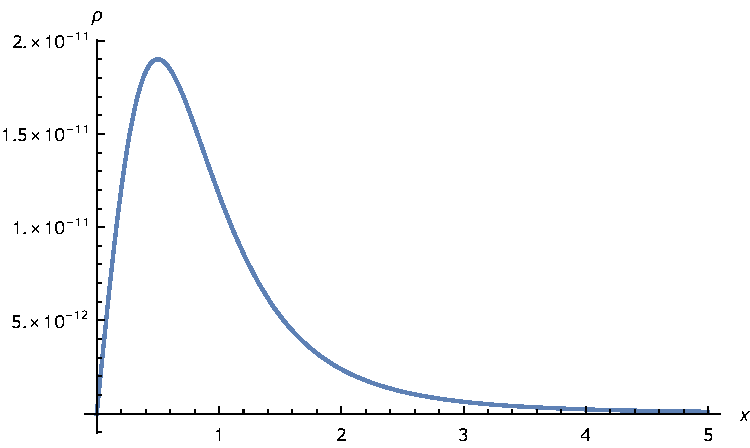
\includegraphics[width=10cm]{classical_electrodynamics/img/ch1/ödev/rho2.pdf}
\caption*{$V_{0} = 5V, a=1br$ alınmıştır.}
	\end{figure}

\newpage
 
   \begin{figure}[h!]
 \centering
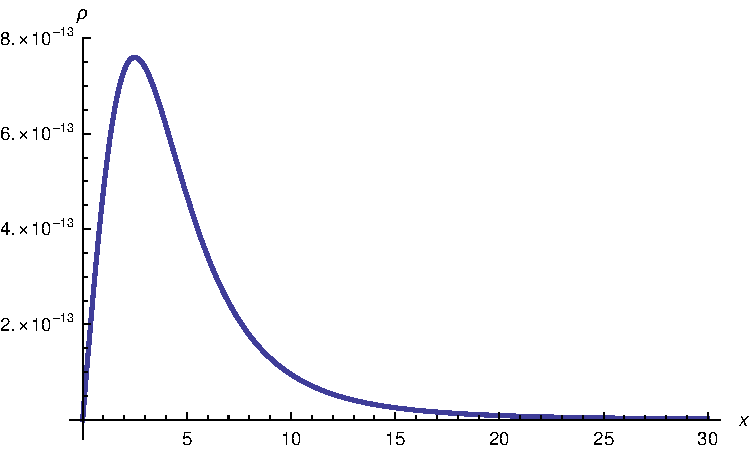
\includegraphics[width=10cm]{classical_electrodynamics/img/ch1/ödev/rho4.pdf}
\caption*{$V_{0} = 5V, a=5br$ alınmıştır.}
	\end{figure}
 
\textbf{c)}
\begin{align}
    \phi(x) = \dfrac{V_{0}}{2} \Big( 1 + \dfrac{x}{\sqrt{x^{2} + a^{2}}} \Big)
\end{align}
\begin{figure}[h]
 \centering
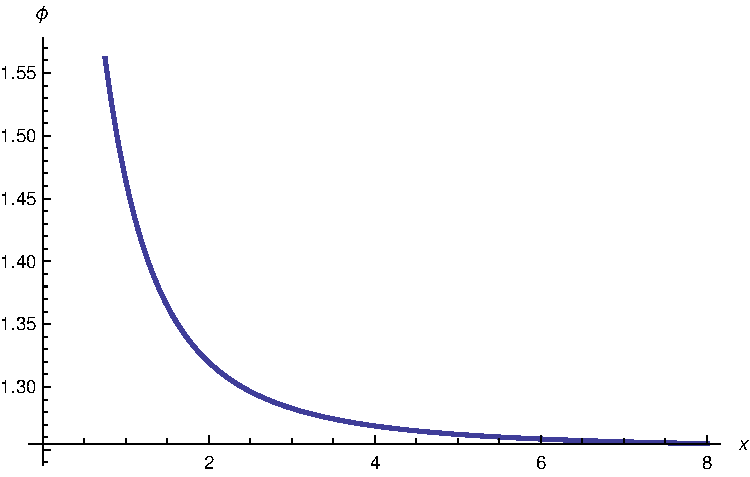
\includegraphics[width=9.5cm]{classical_electrodynamics/img/ch1/ödev/phi1.pdf}
\caption*{$V_{0} = 5V, a=1br$ alınmıştır.}
	\end{figure}
 \begin{figure}[h!]
 \centering
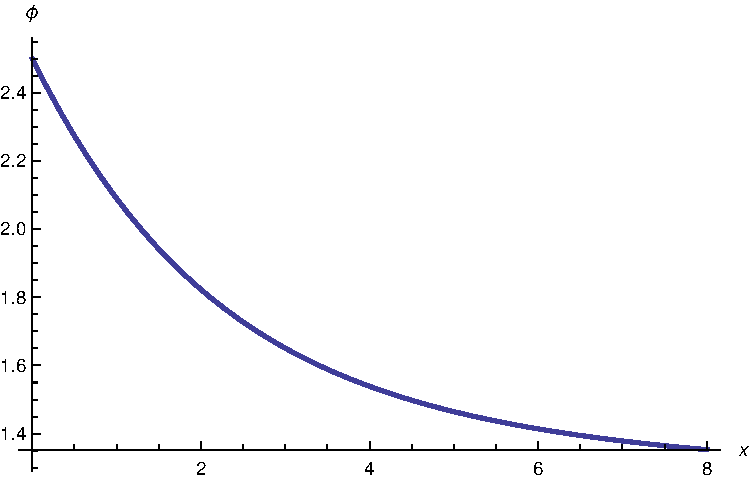
\includegraphics[width=9.5cm]{classical_electrodynamics/img/ch1/ödev/phi2.pdf}
\caption*{$V_{0} = 5V, a=5br$ alınmıştır.}
	\end{figure}

\dangersign \ Soru 2 Jackson 1.14 olup problemler bölümünde verilmiştir.
\cleardoublepage
\setcounter{equation}{0}
\subsection*{Ödev 1.1}

\begin{flushleft}

  
	\textbf{Soru 1:} $ \nabla^{2} \Big( \dfrac{1}{|\Vec{x} - \Vec{x_{1}}|} \Big) $ ifadesini kartezyen koordinatlarda elde ediniz.

	
\end{flushleft}
   
\noindent \textbf{Çözüm:} 

\noindent Kartezyen koordinatlarda $\grad$ operatörü,
\begin{align}
    \grad = \hat{x} \dfrac{\partial}{\partial x} + \hat{y} \dfrac{\partial}{\partial y} + \hat{z} \dfrac{\partial}{\partial z}
\end{align}
Laplasyen,
\begin{align}
  \grad \cdot \grad  =  \nabla^{2} = (  \hat{x} \dfrac{\partial}{\partial x} + \hat{y} \dfrac{\partial}{\partial y} + \hat{z} \dfrac{\partial}{\partial z} ) \cdot (  \hat{x} \dfrac{\partial}{\partial x} + \hat{y} \dfrac{\partial}{\partial y} + \hat{z} \dfrac{\partial}{\partial z} )
\end{align}
\begin{align}
    \nabla^{2} =  \dfrac{\partial^{2}}{\partial x^{2}} + \dfrac{\partial^{2}}{\partial y^{2}} + \dfrac{\partial^{2}}{\partial z^{2}} 
\end{align}
Burada $|\Vec{x} - \Vec{x_{1}}| = r $ olarak alalım,
\begin{align}
    \Vec{r} = x \hat{x} + y \hat{y} + z \hat{z}
\end{align}
\begin{align}
|r| = \sqrt{x^{2} + y^{2}  + z^{2} }
\end{align}
\begin{align}
  \grad(\dfrac{1}{r}) = \grad \big( \dfrac{1}{\sqrt{x^{2} + y^{2} + z^{2}}}  \big) 
\end{align}
\begin{align}
 \grad \big( \dfrac{1}{\sqrt{x^{2} + y^{2} + z^{2}}}  \big) = \big(  \hat{x} \dfrac{\partial}{\partial x} + \hat{y} \dfrac{\partial}{\partial y} + \hat{z} \dfrac{\partial}{\partial z} \big) \big( \dfrac{1}{\sqrt{x^{2} + y^{2} + z^{2}}}  \big)
\end{align}
\begin{align}
&= \hat{x}  \bigg\{ - \dfrac{1}{2} (x^{2} + y^{2} + z^{2})^{-3/2} (2x) \bigg\} \\
&\ + \hat{y} \bigg\{ - \dfrac{1}{2} (x^{2} + y^{2} + z^{2})^{-3/2} (2y) \bigg\} \\
&\ + \hat{z} \bigg\{ - \dfrac{1}{2} (x^{2} + y^{2} + z^{2})^{-3/2} (2z) \bigg\} 
\end{align}
\begin{align}
    = - \dfrac{(x^{2} + y^{2} + z^{2})^{-3/2}}{2}  \bigg\{ 2x \hat{x} + 2y \hat{y} + 2z \hat{z} \bigg\} 
\end{align}
\begin{align}
    = - \dfrac{(x^{2} + y^{2} + z^{2})^{-3/2}}{\cancel{2}} \cancel{2} \bigg\{ x \hat{x} + y \hat{y} + z \hat{z} \bigg\} 
\end{align}

\newpage 
 

\begin{align}
    = - \dfrac{1}{(x^{2} + y^{2} + z^{2})^{3/2}} \bigg\{ x \hat{x} + y \hat{y} + z \hat{z} \bigg\} 
\end{align}
\begin{align}
\grad (\dfrac{1}{r})= -\dfrac{\Vec{r}}{r^{3}}
\end{align}
\begin{align}
|\Vec{x} - \Vec{x_{1}}| = r \rightarrow \grad \dfrac{1}{|\Vec{x} - \Vec{x}_{1}|}= - \dfrac{(\Vec{x} - \Vec{x_{1}})}{|\Vec{x} - \Vec{x_{1}}|^{3}}
\end{align}
\begin{align}
 \nabla^{2} \Big( \dfrac{1}{|\Vec{x} - \Vec{x_{1}}|} \Big) = - \grad \cdot \bigg( \dfrac{(\Vec{x} - \Vec{x_{1}})}{|\Vec{x} - \Vec{x_{1}}|^{3}} \bigg)
\end{align}

Diverjans için çarpım kuralını kullanmamız gerekecek,
\begin{align*}
    \grad \cdot (f \Vec{A}) = \dfrac{\partial}{\partial x} (f A_{x}) + \dfrac{\partial}{\partial y} (f A_{y}) + \dfrac{\partial}{\partial z} (f A_{z})
\end{align*}
\begin{align*}
    = \bigg(  \dfrac{\partial f}{\partial x} A_{x} + f \dfrac{\partial A_{x}}{\partial x} \bigg) + \bigg(  \dfrac{\partial f}{\partial y} A_{y} + f \dfrac{\partial A_{y}}{\partial y} \bigg) + \bigg(  \dfrac{\partial f}{\partial z} A_{z} + f \dfrac{\partial A_{z}}{\partial z} \bigg)
\end{align*}
\begin{align}
\grad \cdot (f \Vec{A}) = f (\grad \cdot \Vec{A}) + \Vec{A} \cdot (\grad f)  
\end{align}

Denklem (1.17)'deki çarpım kuralı Denklem (1.16)'da yerine konulursa, (-'yi daha sonra dahil edebiliriz)

\begin{align}
\grad \cdot \bigg( \dfrac{(\Vec{x} - \Vec{x_{1}})}{|\Vec{x} - \Vec{x_{1}}|^{3}} \bigg) = \bigg( \dfrac{1}{|\Vec{x} - \Vec{x_{1}}|^{3}} \bigg) \grad \cdot (\Vec{x} - \Vec{x_{1}}) + (\Vec{x} - \Vec{x_{1}}) \cdot \grad \bigg( \dfrac{1}{|\Vec{x} - \Vec{x_{1}}|^{3}} \bigg)
\end{align}

İlk olarak $\grad \cdot (\Vec{x} - \Vec{x_{1}})$ terimini hesaplayalım,
\begin{align}
    \grad \cdot (\Vec{x} - \Vec{x_{1}}) =  \big(  \hat{x} \dfrac{\partial}{\partial x} + \hat{y} \dfrac{\partial}{\partial y} + \hat{z} \dfrac{\partial}{\partial z} \big) \cdot (\Vec{x} - \Vec{x_{1}}) = 3
\end{align}
İkinci olarak $ \grad \bigg( \dfrac{1}{|\Vec{x} - \Vec{x_{1}}|^{3}} \bigg)$ terimini hesaplayalım. Burada kolaylık olması açısından tekrardan $|\Vec{x} - \Vec{x_{1}}| = r $ olarak almaktayız,
\begin{align}
  \grad(\dfrac{1}{r^{3}}) = \grad \dfrac{1}{ \big( x^{2} + y^{2} + z^{2} \big)^{3/2} }
\end{align}
\begin{align}
 \grad \Big( \dfrac{1}{\big(x^{2} + y^{2} + z^{2} \big)^{3/2}}  \Big) = \big(  \hat{x} \dfrac{\partial}{\partial x} + \hat{y} \dfrac{\partial}{\partial y} + \hat{z} \dfrac{\partial}{\partial z} \big) \big( \dfrac{1}{\big( {x^{2} + y^{2} + z^{2}} \big)^{3/2}}  \big)
\end{align}
\begin{align*}
&= \hat{x}  \bigg\{ - \dfrac{3}{2} (x^{2} + y^{2} + z^{2})^{-5/2} (2x) \bigg\} \\
&\ + \hat{y} \bigg\{ - \dfrac{3}{2} (x^{2} + y^{2} + z^{2})^{-5/2} (2y) \bigg\} \\
&\ + \hat{z} \bigg\{ - \dfrac{3}{2} (x^{2} + y^{2} + z^{2})^{-5/2} (2z) \bigg\} 
\end{align*}
\begin{align}
    = - 3 \dfrac{(x^{2} + y^{2} + z^{2})^{-5/2}}{2}  \bigg\{ 2x \hat{x} + 2y \hat{y} + 2z \hat{z} \bigg\} 
\end{align}
\begin{align}
    = - 3 \dfrac{(x^{2} + y^{2} + z^{2})^{-5/2}}{\cancel{2}} \cancel{2} \bigg\{ x \hat{x} + y \hat{y} + z \hat{z} \bigg\} 
\end{align}
\begin{align}
\grad (\dfrac{1}{r^{3}})= -\dfrac{3 \Vec{r}}{r^{5}}
\end{align}

\newpage

\begin{align}
|\Vec{x} - \Vec{x_{1}}| = r \rightarrow \ \grad \bigg( \dfrac{1}{|\Vec{x} - \Vec{x_{1}}|^{3}} \bigg) = - \dfrac{3 (\Vec{x} - \Vec{x_{1}})}{|\Vec{x} - \Vec{x_{1}}|^{5}}
\end{align}

Hesapladığımız terimleri Denklem (1.18)'de yerine yazalım,

\begin{align}
\grad \cdot \bigg( \dfrac{(\Vec{x} - \Vec{x_{1}})}{|\Vec{x} - \Vec{x_{1}}|^{3}} \bigg) = \bigg( \dfrac{1}{|\Vec{x} - \Vec{x_{1}}|^{3}} \bigg) \underbrace{\grad \cdot (\Vec{x} - \Vec{x_{1}})}_{3} + (\Vec{x} - \Vec{x_{1}}) \cdot \underbrace{\grad \bigg( \dfrac{1}{|\Vec{x} - \Vec{x_{1}}|^{3}} \bigg)}_{- \dfrac{3 (\Vec{x} - \Vec{x_{1}})}{|\Vec{x} - \Vec{x_{1}}|^{5}}}
\end{align}
\begin{align}
\grad \cdot \bigg( \dfrac{(\Vec{x} - \Vec{x_{1}})}{|\Vec{x} - \Vec{x_{1}}|^{3}} \bigg) = \bigg( \dfrac{1}{|\Vec{x} - \Vec{x_{1}}|^{3}} \bigg) 3 + (\Vec{x} - \Vec{x_{1}}) \cdot \bigg( - \dfrac{3 (\Vec{x} - \Vec{x_{1}})}{|\Vec{x} - \Vec{x_{1}}|^{5}} \bigg)
\end{align}
\begin{align}
\grad \cdot \bigg( \dfrac{(\Vec{x} - \Vec{x_{1}})}{|\Vec{x} - \Vec{x_{1}}|^{3}} \bigg) =  \dfrac{3}{|\Vec{x} - \Vec{x_{1}}|^{3}}   - \dfrac{3 |\Vec{x} - \Vec{x_{1}}|^{2}}{|\Vec{x} - \Vec{x_{1}}|^{5}} 
\end{align}
-'yi dahil edip sonucu yazalım,
\begin{align}
- \grad \cdot \bigg( \dfrac{(\Vec{x} - \Vec{x_{1}})}{|\Vec{x} - \Vec{x_{1}}|^{3}} \bigg) =  - \dfrac{3}{|\Vec{x} - \Vec{x_{1}}|^{3}}  + \dfrac{3}{|\Vec{x} - \Vec{x_{1}}|^{3}} = 0
\end{align}
Yani,
\begin{align}
\nabla^{2} \Big( \dfrac{1}{|\Vec{x} - \Vec{x_{1}}|} \Big) =  - \grad \cdot \bigg( \dfrac{(\Vec{x} - \Vec{x_{1}})}{|\Vec{x} - \Vec{x_{1}}|^{3}} \bigg) = 0
\end{align}



\newpage


\begin{flushleft}
	\textbf{Soru 2:} $ 0 < r < R$'de tanımlı bir küresel bölge $\rho = \dfrac{K}{r}$ yük yoğunluğuna sahiptir, burada K bir sabittir. Kürenin içinde ve dışında elektrik alanı ve potansiyeli bulunuz. Bulduğunuz potansiyeller için Poisson denklemlerini elde ederek sonucu yorumlayınız.
\end{flushleft}
   
	\textbf{Çözüm:} 
Karışıklık olmaması adına kürenin yarıçapına $r_{0}$ diyelim. Kürenin dışı için elektrik alanı bulmak için $r$ yarıçaplı bir Gauss yüzeyi alalım,
\begin{align*}
 \oint \Vec{E} \cdot d\Vec{a} = \dfrac{Q_{\textrm{iç}}}{ \varepsilon_{0}}
\end{align*}
\[  \oint_{S} \Vec{E} \cdot d\Vec{a} = \oint_{S} |\Vec{E}| da \]
\[\oint_{S}  |\Vec{E}| da =  |\Vec{E}| \oint_{S} da =  |\Vec{E}| 4 \pi r^{2} \]
\[ Q = \int \rho dV  = \int_{0}^{r_{0}} \int_{0}^{\pi}  \int_{0}^{2 \pi} \dfrac{K}{r} r^{2} \sin \theta dr d\theta d \phi \]
\[ Q =  K \int_{0}^{r_{0}}  r dr \int_{0}^{\pi} \sin \theta d\theta  \int_{0}^{2 \pi} d \phi \]
\[ =  K  \Bigg\{ \dfrac{r^{2}}{2} \Bigg|_{0}^{r_{0}} \Bigg\} \Bigg\{ - \cos \theta \Bigg|_{0}^{\pi} \Bigg\}  \Bigg\{ \phi \Bigg|_{0}^{2 \pi} \Bigg\} \]
\[ =  K  \Bigg\{ \dfrac{r_{0}^{2}}{2} \Bigg\} \Bigg\{ - \cos \pi + \cos 0 \Bigg\}  \Bigg\{ 2 \pi - 0 \Bigg\} \]
\[ =  K  \Bigg\{ \dfrac{r_{0}^{2}}{2} \Bigg\} \Bigg\{ 1 + 1 \Bigg\}  \Bigg\{ 2 \pi - 0 \Bigg\}  = K  \dfrac{r_{0}^{2}}{2} 4 \pi \]
\[ Q =  K  \dfrac{r_{0}^{2}}{2} 4 \pi\]
\[ \oint \Vec{E} \cdot d\Vec{a} = \dfrac{\sum Q_{\text{iç}}}{\varepsilon_{0}}  \]
\[ |\Vec{E}| 4 \pi r^{2} = \dfrac{1}{\varepsilon_{0}}  K  \dfrac{r_{0}^{2}}{2} 4 \pi \]
\[ |\Vec{E}|  = \dfrac{1}{ 4 \pi r^{2} \varepsilon_{0}}   K  \dfrac{r_{0}^{2}}{2}  4 \pi = \dfrac{1}{\varepsilon_{0}}\ \dfrac{K}{2} \dfrac{r_{0}^{2}}{r^{2}}\]
\[ \Vec{E} = \dfrac{1}{\varepsilon_{0}}\ \dfrac{K}{2} \dfrac{r_{0}^{2}}{r^{2}} \hat{r} \]
Kürenin dışında elektrik potansiyelini hesaplayalım,
\[ V_{b} - V_{a} = \Delta V = - \int_{a}^{b} \Vec{E} \cdot d \Vec{l} \]
Aslında burada $\theta$ ve $\phi$'de vektördür.
\[ d \Vec{l} = d \Vec{r} + r d \Vec{\theta} + r \sin \theta d \phi \]
\[ d \Vec{r} =\hat{r} dr \]
\[ V_{r} - \cancelto{0}{V_{\infty}}  = - \int_{\infty}^{r} \Vec{E} \cdot d \Vec{l} \]
\[ V_{r}  = - \int_{\infty}^{r}  \dfrac{1}{\varepsilon_{0}} \dfrac{K}{2} \dfrac{r_{0}^{2}}{r^{2}} \underbrace{ \hat{r} \cdot \hat{r}}_{1} dr \]
\[ V_{r}  = - \dfrac{r_{0}^{2}}{\varepsilon_{0}} \dfrac{K}{2} \int_{\infty}^{r}   \dfrac{1}{r'^{2}} dr' \]
\[ V_{r}  = - \dfrac{r_{0}^{2}}{\varepsilon_{0}} \dfrac{K}{2} \Bigg\{ \dfrac{r'^{-1}}{-1} \Bigg|_{\infty}^{r} \Bigg\} \]
\[ V_{r}  = - \dfrac{r_{0}^{2}}{\varepsilon_{0}} \dfrac{K}{2} \Bigg\{ - \dfrac{1}{r} + \cancelto{0}{\dfrac{1}{\infty}} \Bigg\} \]
\[ V_{r}  =  \dfrac{r_{0}^{2}}{\varepsilon_{0}} \dfrac{K}{2} \dfrac{1}{r}  \]
\[ \nabla^{2}V = - \dfrac{\rho}{\varepsilon_{0}} \]
\[  \dfrac{r_{0}^{2}}{\varepsilon_{0}} \dfrac{K}{2} \nabla^{2} (\dfrac{1}{r}) = - \dfrac{\rho}{\varepsilon_{0}} \]
Burada,
\[ \nabla^{2} (\dfrac{1}{r}) = - 4 \pi \delta (r) \textrm{'dir.} \]
\[  \dfrac{r_{0}^{2}}{\varepsilon_{0}} \dfrac{K}{2} ( - 4 \pi \delta (r) ) = - \dfrac{\rho}{\varepsilon_{0}} \]
\[ \rho = r_{0}^{2} K 2 \pi \delta (r) \]
Kürenin içinde elektrik alanı bulmak için yine $r$ yarıçaplı bir Gauss yüzeyi alalım,
\begin{align*}
 \oint \Vec{E} \cdot d\Vec{a} = \dfrac{Q_{\text{iç}}}{ \varepsilon_{0}}
\end{align*}
\[  \oint_{S} \Vec{E} \cdot d\Vec{a} = \oint_{S} |\Vec{E}| da \]
\[\oint_{S}  |\Vec{E}| da =  |\Vec{E}| \oint_{S} da =  |\Vec{E}| 4 \pi r^{2} \]
\[ Q = \int \rho dV  = \int_{0}^{r} \int_{0}^{\pi}  \int_{0}^{2 \pi} \dfrac{K}{r} r^{2} \sin \theta dr d\theta d \phi \]
Hem içeride, hem de integralin sınırlarında $r$ olduğu için integralin içindeki $r$'leri $r'$ olarak gösterelim,
\[ Q =  K \int_{0}^{r}  r' dr' \int_{0}^{\pi} \sin \theta d\theta  \int_{0}^{2 \pi} d \phi \]
\[ =  K  \Bigg\{ \dfrac{r'^{2}}{2} \Bigg|_{0}^{r} \Bigg\} \Bigg\{ - \cos \theta \Bigg|_{0}^{\pi} \Bigg\}  \Bigg\{ \phi \Bigg|_{0}^{2 \pi} \Bigg\} \]
\[ =  K  \Bigg\{ \dfrac{r^{2}}{2} \Bigg\} \Bigg\{ - \cos \pi + \cos 0 \Bigg\}  \Bigg\{ 2 \pi - 0 \Bigg\} \]
\[ =  K  \Bigg\{ \dfrac{r^{2}}{2} \Bigg\} \Bigg\{ 1 + 1 \Bigg\}  \Bigg\{ 2 \pi - 0 \Bigg\}  = K  \dfrac{r^{2}}{2} 4 \pi \]
\[ Q =  K  \dfrac{r^{2}}{2} 4 \pi\]
\[ \oint \Vec{E} \cdot d\Vec{a} = \dfrac{Q}{\varepsilon_{0}}  \]
\[ |\Vec{E}| 4 \pi r^{2} = \dfrac{1}{\varepsilon_{0}}  K  \dfrac{r^{2}}{2} 4 \pi \]
\[ |\Vec{E}|  = \dfrac{1}{ 4 \pi r^{2} \varepsilon_{0}}   K  \dfrac{r^{2}}{2}  4 \pi = \dfrac{1}{\varepsilon_{0}}\ \dfrac{K}{2}\]
\[ \Vec{E} = \dfrac{1}{\varepsilon_{0}}\ \dfrac{K}{2} \hat{r} \]
Kürenin içinde elektrik potansiyelini hesaplayalım,
\[ V_{b} - V_{a} = \Delta V = - \int_{a}^{b} \Vec{E} \cdot d \Vec{l} \]
% \[ V_{r} - V_{r_{0}}  = - \int_{\infty}^{r} \Vec{E} \cdot d \Vec{l} - \int_{r_{0}}^{r} \Vec{E} \cdot d \Vec{l} \]
\[ V_{r} - V_{r_{0}}  = - \int_{r_{0}}^{r} \Vec{E} \cdot d \Vec{l} \]
\[  = - \int_{r_{0}}^{r} \dfrac{1}{\varepsilon_{0}}\ \dfrac{K}{2} \underbrace{ \hat{r} \cdot \hat{r}}_{1} dr' \]
\[  = - \dfrac{1}{\varepsilon_{0}}\ \dfrac{K}{2} \int_{r_{0}}^{r} dr' = - \dfrac{1}{\varepsilon_{0}}\ \dfrac{K}{2} \Bigg\{ r' \Bigg|_{r_{0}}^{r} \Bigg\} \]
\[ =  - \dfrac{1}{\varepsilon_{0}}\ \dfrac{K}{2} \Bigg\{ r' \Bigg|_{r_{0}}^{r} \Bigg\} =  - \dfrac{1}{\varepsilon_{0}}\ \dfrac{K}{2} \Bigg\{ r  - r_{0} \Bigg\} \]
\[ V_{r} - V_{r_{0}} =  - \dfrac{r}{\varepsilon_{0}}\ \dfrac{K}{2} + \dfrac{r_{0}}{\varepsilon_{0}}\ \dfrac{K}{2} \]
\[ V_{r=r_{0}} =  \dfrac{r_{0}^{2}}{\varepsilon_{0}} \dfrac{K}{2} \dfrac{1}{r_{0}} = \dfrac{r_{0}}{\varepsilon_{0}} \dfrac{K}{2} \]
\[ V_{r} - \dfrac{r_{0}}{\varepsilon_{0}} \dfrac{K}{2}  =  - \dfrac{r}{\varepsilon_{0}}\ \dfrac{K}{2} + \dfrac{r_{0}}{\varepsilon_{0}}\ \dfrac{K}{2} \]
\[ V_{r}  =  - \dfrac{r}{\varepsilon_{0}}\ \dfrac{K}{2} + \dfrac{r_{0}}{\varepsilon_{0}}\ \dfrac{K}{2}  + \dfrac{r_{0}}{\varepsilon_{0}} \dfrac{K}{2}\]
\[ V_{r}  = \dfrac{1}{\varepsilon_{0}}\ \dfrac{K}{2} \Bigg\{ 2 r_{0} - r \Bigg\} \]
\[ \nabla^{2}V = - \dfrac{\rho}{\varepsilon_{0}} \]
\newpage



\begin{flushleft}
   
	\textbf{Soru 3:} Keyfi bir F skaleri için $\grad \times \big(\grad F \big) $ ifadesini kartezyen koordinatlarda hesaplayınız. F fonksiyonunun 2. mertebeden kısmi türevleri süreklidir.

\end{flushleft}

  
   
	\textbf{Çözüm:} 

 $\grad \times \big(\grad F \big) $ ifadesi aslında gradyanın rotasyonelidir.
\begin{align}
    \grad F (x,y,z) = (  \hat{x} \dfrac{\partial}{\partial x} + \hat{y} \dfrac{\partial}{\partial y} + \hat{z} \dfrac{\partial}{\partial z} ) F
\end{align}
\begin{align}
    \grad F (x,y,z) = (  \hat{x} \dfrac{\partial F}{\partial x} + \hat{y} \dfrac{\partial F}{\partial y} + \hat{z} \dfrac{\partial F}{\partial z} ) 
\end{align}
 \begin{align}
    \grad F  = (  \dfrac{\partial F}{\partial x} +  \dfrac{\partial F}{\partial y} +  \dfrac{\partial F}{\partial z} ) 
\end{align}
\begin{align}
\grad  \times ( \grad F ) = \grad \times \Vec{F} =  
\begin{vmatrix}
 \hat{x} & \hat{y} & \hat{z} \\
 \dfrac{\partial}{\partial x} & \dfrac{\partial}{\partial y} & \dfrac{\partial}{\partial z} \\[2ex]
\dfrac{\partial F}{\partial x} & \dfrac{\partial F}{\partial y} & \dfrac{\partial F}{\partial z}
 \end{vmatrix}
\end{align}
\begin{align}
= \Big\{ \dfrac{\partial}{\partial y} \big( \dfrac{\partial F}{\partial z} \big) - \dfrac{\partial}{\partial z} \big( \dfrac{\partial F}{\partial y} \big) \Big\} \hat{x} - \Big\{ \dfrac{\partial}{\partial x} \big( \dfrac{\partial F}{\partial z} \big) - \dfrac{\partial}{\partial z} \big( \dfrac{\partial F}{\partial x} \big) \Big\} \hat{y} + \Big\{ \dfrac{\partial}{\partial x} \big( \dfrac{\partial F}{\partial y} \big) - \dfrac{\partial}{\partial y} \big( \dfrac{\partial F}{\partial x} \big) \Big\} \hat{z}
\end{align}
\begin{align}
= \Big\{ \dfrac{\partial^{2} F}{\partial y \partial z}  - \dfrac{\partial^{2} F}{\partial z \partial y} \Big\} \hat{x} - \Big\{ \dfrac{\partial^{2} F}{\partial x \partial z}  - \dfrac{\partial^{2} F}{\partial z \partial x} \Big\} \hat{y} + \Big\{ \dfrac{\partial^{2} F}{\partial x \partial y}  - \dfrac{\partial^{2} F}{\partial y \partial x} \Big\} \hat{z}
\end{align}
$ \therefore$ Eğer F fonksiyonunun ikinci mertebeden kısmi türevleri sürekli ise Clairaut teoreminden
\begin{align}
\dfrac{\partial^{2} F}{\partial x \partial y} = \dfrac{\partial^{2} F}{\partial y \partial x}
\end{align}
eşitliğini elde ederiz. Burada karışık kısmi türevlerin eşitliğini kullanıyoruz. Böylece,
\begin{align}
 \dfrac{\partial^{2} F}{\partial y \partial z}  = \dfrac{\partial^{2} F}{\partial z \partial y} , \ 
 \dfrac{\partial^{2} F}{\partial x \partial z}  = \dfrac{\partial^{2} F}{\partial z \partial x} , \
 \dfrac{\partial^{2} F}{\partial x \partial y}  = \dfrac{\partial^{2} F}{\partial y \partial x} 
\end{align}
eşitliklerini elde ediriz. Elde edilen terimler Denklem (1.37)'de yerine yazılırsa,
\begin{align}
\grad  \times ( \grad F ) = \grad \times \Vec{F} =
\Big\{ \dfrac{\partial^{2} F}{\partial y \partial z}  - \dfrac{\partial^{2} F}{\partial y \partial z} \Big\} \hat{x} - \Big\{ \dfrac{\partial^{2} F}{\partial x \partial z}  - \dfrac{\partial^{2} F}{\partial x \partial z} \Big\} \hat{y} + \Big\{ \dfrac{\partial^{2} F}{\partial x \partial y}  - \dfrac{\partial^{2} F}{\partial x \partial y} \Big\} \hat{z}
\end{align}
\begin{align}
= \Big\{ 0 \Big\} \hat{x} - 
\Big\{ 0 \Big\} \hat{y} + 
\Big\{ 0 \Big\} \hat{z} = 0
\end{align}
\begin{align}
    \therefore \grad  \times ( \grad F ) = 0
\end{align}